
\documentclass[color=green,titlestyle=hang]{elegantbook}%cyan,mathpazo,

\author{唐绍东 \& TangShaodong}
\email{1096084877@qq.com}
\zhtitle{微积分}
\zhend{备注}
\entitle{Calculus }
\enend{note}
\version{3.10}
\myquote{Victory won\rq t come to us unless we go to it.}
\logo{logo.png}
\cover{cover.pdf}

%green color
\definecolor{main1}{RGB}{0,120,2}
\definecolor{seco1}{RGB}{230,90,7}
\definecolor{thid1}{RGB}{0,160,152}
%cyan color
\definecolor{main2}{RGB}{0,175,152}
\definecolor{seco2}{RGB}{239,126,30}
\definecolor{thid2}{RGB}{120,8,13}
%blue color
\definecolor{main3}{RGB}{20,50,104}
\definecolor{seco3}{RGB}{180,50,131}
\definecolor{thid3}{RGB}{7,127,128}


\usepackage{makecell}
\usepackage{lipsum}
\RequirePackage{calc}
\allowdisplaybreaks[4]%%%公式换页
\usepackage{cases}%\begin{numcases}{}编号
\usepackage{scalerel} %\scaleobj{1.5}{} 缩放公式大小
\usepackage{texnames}
\usepackage{tabularx}
\usepackage{CJKfntef}%修饰汉字画波浪线下划线删除线
%\CJKunderwave{汉字,波浪线}\CJKunderdot{汉字,下加点}\CJKunderdlline{汉字,下双线}
\usepackage{fancybox}
\usepackage{pgfplots}%axis环境%\pgfplotsset{compat=1.8}
\usepgfplotslibrary{fillbetween}
\usetikzlibrary{patterns}
\usetikzlibrary{intersections}
\usetikzlibrary{quotes,angles}
\usetikzlibrary{datavisualization.polar,arrows}	
\usetikzlibrary{datavisualization.formats.functions}
%\pgfplotsset{width=7cm,compat=1.14}

\begin{document}
\maketitle
\tableofcontents
\mainmatter


\begin{example}
已知函数 $f(x)$ 满足关系式
\[af(x)+f\left(\frac{1}{x}\right)=\frac{b}{x}\quad(|a|\neq1\,,\;a\,,\;b,\,,\; \text{为常数})\]
确定 $f(x)$ 的奇偶性
\end{example}\begin{solution}
将 $x=\frac{1}{t}$ 代入关系式得 $af\left(\frac{1}{t}\right)+f(t)=bt$,
又将 $t$ 改为 $x$ 与关系式联立方程组
\[\begin{cases*}
af(x)+f\left(\frac{1}{x}\right)=\frac{b}{x}\\
af(x)+f(x)=\frac{b}{x}
\end{cases*}\]
可解得
\[f(x)=\frac{1}{a^2-1}\left(\frac{ab}{x}-bx\right)=\frac{ab-bx^2}{(a^2-1)x}\;(a\neq1)\,.\]
显然\[f(-x)=\frac{ab-b(-x)^2}{(a^2-1)(-x)}=-f(x)\]
所以 $f(x)$ 是奇函数
\end{solution}

\chapter{极限}

\begin{example}
利用定义证明 $\lim\limits_{n\to \infty}c=c$
\end{example}\begin{proof}
$\forall \varepsilon >0$, 因为 $$|x_n-c|=|c-c|=0,$$
所以对任意的自然数 $n$, 都有 $|x_n-c|<\varepsilon,$ 即 $\lim\limits_{n\to \infty}c=c$.	
\end{proof}

\begin{example}
利用定义证明 $\lim\limits_{n\to \infty}\frac{(-1)^n}{n}=0$.
\end{example}\begin{proof}
首先有 $$|x_n-0|=\Big|\frac{(-1)^n}{n}-0\Big|=\frac{1}{n}.$$ 因此 $\forall \varepsilon >0$,
要使 $|x_n-0|<\varepsilon$, 只需要 $\frac{1}{n}<\varepsilon$, 即 $n>\frac{1}{\varepsilon}$.
故取正整数 $N=\Big[\frac{1}{\varepsilon}\Big]+1$, \\
则当 $n>N$ 时, 就有$$\Big|\frac{(-1)^n}{n}-0\Big|<\varepsilon,$$
即 $\lim\limits_{n\to \infty}\frac{(-1)^n}{n}=0$. 证毕.	
\end{proof}

\begin{example}
利用定义证明  $\lim\limits_{n\to \infty}q^{n-1}=0$.	
\end{example}\begin{proof}
由于 $$|x_n-0|=|q^{n-1}-0|=|q|^{n-1},$$ 因此 $\forall \varepsilon >0,$
要使 $|x_n-0|<\varepsilon$, 只要
$$|q|^{n-1}<\varepsilon.$$
两边取自然对数, 得 $$(n-1)\ln|q|<\ln\varepsilon.$$  因 $|q|<1, \ln|q|<0,$
故
$$n>\frac{\ln\varepsilon}{\ln|q|}+1.$$
当 $\varepsilon>1$ 时, $\frac{\ln \varepsilon}{\ln|q|}$ 是负数, 这时可取 $N=1$. 当 $\varepsilon<1$ 时, 取
$$N=\Big[\frac{\ln \varepsilon}{\ln|q|}+1\Big],$$
则当 $n>N$ 时, 就有
$$|q^{n-1}-0|<\varepsilon,$$
即 $\lim\limits_{n\to \infty}q^{n-1}=0$. 证毕.	
\end{proof}

\begin{example}
用定义验证: $\lim_{n\to\infty}\frac{n^2}{3n^2-n-7}=\frac{1}{3}$. 
\end{example}\begin{proof}
任给 $\varepsilon>0$, 由	
\[\left|\frac{n^2}{3n^2n-7}-\frac{1}{3}\right|=\frac{n+7}{3(3n^2-n-7)}\]
{\color{blue}当 $n\geqslant7$ 时}, $n+7\leqslant2n$, $3n^2-n-7\geqslant3n^2-2n\geqslant 2n^2$\\
故要使\[\left|\frac{n^2}{3n^2n-7}-\frac{1}{3}\right|\leqslant\frac{2n}{6n^2}=\frac{1}{3n}<\varepsilon\]
只要 $n>\frac{1}{3\varepsilon}$ 即可.\\
对于任意的正数 $\varepsilon$ , 取 {\color{blue}$N=\max\Big\{7,\big[\tfrac{1}{3\varepsilon}\big]\Big\}$}, 当 $n>N$ 时, 有\[\left|\frac{n^2}{3n^2-n-7}-\frac{1}{3}\right|<\varepsilon\]
即得\[\lim_{n\to\infty}\frac{n^2}{3n^2-n-7}=\frac{1}{3}\]
\end{proof}

\begin{property}
有限个无穷小的和仍是无穷小.
\end{property}

\begin{property}
有限个无穷小的乘积仍是无穷小.	
\end{property}

\begin{property}
有界函数和无穷小的乘积是无穷小.	
\end{property}\begin{proof}
设函数 $u(x)$ 在 $x_0$ 的某一去心邻域 $\overset{\circ}{U}(x_0,\delta_1)$ 内是有界的, \\
即 $\exists M>0$ 使得 $|u(x)|\leqslant M$ 对一切 $x\in \overset{\circ}{U}(x_0,\delta_1)$ 成立. 又设 $\alpha$ 是当 $x\to x_0$ 时的无穷小, \\
即 $\forall \varepsilon>0,\exists \delta_2>0,$ 当 $x\in \overset{\circ}{U}(x_0,\delta_2)$ 时, 有
$$|\alpha|<\frac{\varepsilon}{M}.$$
取 $\delta={\rm {min}}\{\delta_1,\delta_2\},$ 则当 $x\in \overset{\circ}{U}(x_0,\delta)$ 时,
$$|u|\leqslant M\quad \mbox{和}\quad |\alpha|<\frac{\varepsilon}{M}$$
同时成立. 从而
$$|u\alpha|=|u||\alpha|<M\cdot\frac{\varepsilon}{M}=\varepsilon.$$
即 $\lim\limits_{x\to x_0}u\alpha=0$.
\end{proof}

% 无穷多个无穷小量的乘积不一定是无穷小量.

\begin{example}
设数列~$a_n$~满足级数~$|a_1|+|a_2|+\cdots+|a_n|+\cdots$~收敛,\\ 证明:~$\displaystyle\lim_{p\to\infty}(|a_1|^p+|a_2|^p+\cdots+|a_n|^p+\cdots)^{\frac{1}{p}}$~的极限存在, 并求之.
\end{example}\begin{proof}
记\[||a||_p=\left(|a_1|^p+|a_2|^p+\cdots+|a_n|^p+\cdots\right)^{\frac{1}{p}}, ~(p>0)\]
由于~$|a_1|+|a_2|+\cdots+|a_n|+\cdots$ 收敛, 所以$\displaystyle\lim_{n\to\infty}|a_n|=0, \sup|a_n|$存在\\
易证~$|a_n|\leq ||a||_q~(q>1, n=1,2,3,\cdots)$, 于是~$\sup |a_n|\leq ||a||_q$, 对~$1<q<p$
\begin{align*}
||a||_p&=(|a_1|^p+|a_2|^p+\cdots+|a_n|^p+\cdots)^{\frac{1}{p}}\\
&=  (|a_1|^{p-q}|a_1|^q+|a_2|^{p-q}|a_2|^q+\cdots+|a_n|^{p-q}|a_n|^q+\cdots)^{\frac{1}{p}}\\
&\leq ||a||_q^{\frac{p-q}{p}}(|a_1|^q+|a_2|^q+\cdots+|a_n|^q+\cdots)^{\frac{1}{p}}\\
&\leq ||a||_q^{\frac{p-q}{p}}||a||_q^{\frac{q}{p}}=||a||_q
\end{align*}
故~$||a||_p \leq ||a||_q$, 所以~$||a||_p$~关于~$p$~单调递减且有下界.
于是有
\[a_n\leq ||a||_p\leq (\sup a_n)^{1-\frac{q}{p}}||a||_q^{\frac{q}{p}}\]
当~$p\to+\infty$~时, 有夹逼定理, $\displaystyle\lim_{p\to+\infty}||a||_p=\sup |a_n|$	
\end{proof}

%\begin{example}
%设 $x_n=\sqrt{1+\frac{1}{n^{k}}}\;(k\in {\bf N}^+)$, 用定义证明 $\lim\limits_{n\to \infty}x_n=1$.	
%\end{example}\begin{proof}
%首先,
%$$|x_n-1|=\left|\sqrt{1+\frac{1}{n^{k}}}-1\right|=\sqrt{1+\frac{1}{n^{k}}}-1=\frac{\dfrac{1}{n^k}}{\sqrt{1+\frac{1}{n^{k}}}+1}<\frac{1}{2n^k}<\frac{1}{n}.$$
%因此 $\forall 0<\varepsilon <1,$ 要使 $|x_n-1|<\varepsilon$, 只要 $\frac{1}{n}<\varepsilon$, 即 $n>\frac{1}{\varepsilon}$.
%故取正整数 $N=\Big[\frac{1}{\varepsilon}\Big]$, \\
%则当 $n>N$ 时, 就有 $\frac{1}{n}<\varepsilon$, 从而有
%$$\left|\sqrt{1+\frac{1}{n^{k}}}-1\right|<\varepsilon,$$
%即 $\lim\limits_{n\to \infty}x_n=1$. 证毕.	
%\end{proof}

\begin{example}
利用定义证明 $\lim\limits_{n\to\infty}\frac{3n-1}{2n+1}=\frac{3}{2}$.
\end{example}\begin{proof}
首先有 \[\left|\frac{3n-1}{2n+1}-\frac{3}{2}\right|=\frac{5}{2(2n+1)}<\frac{5}{4n}.\]
因此 $\forall \varepsilon >0$,
要使 $\left|\frac{3n-1}{2n+1}-\frac{3}{2}\right|<\varepsilon$, 只需要 $\frac{5}{4n}<\varepsilon$, 即 $n>\frac{5}{4\varepsilon}$.
故取正整数 $N=\Big\lfloor\frac{5}{4\varepsilon}\Big\rfloor$, \\
则当 $n>N$ 时, 就有\[\left|\frac{3n-1}{2n+1}-\frac{3}{2}\right|<\varepsilon,\]
即 $\lim\limits_{n\to\infty}\frac{3n-1}{2n+1}=\frac{3}{2}$. 		
\end{proof}

\begin{example}
用定义证明:  $\lim_{n\to\infty}\frac{n+2}{n^2-2}\sin n=0$
\end{example}\begin{solution}
首先有 \[\left|\frac{n+2}{n^2-2}\sin n-0\right|\leqslant\left|\frac{n+2}{n^2-2}\right|<\frac{n+2}{n^2-4}=\frac{1}{n-2}\,,\;n\geqslant3\]
因此, $\forall \varepsilon >0$,
要使 $\left|\frac{n+2}{n^2-2}\sin n-0\right|<\varepsilon$, 只需要 $\frac{1}{n-2}<\varepsilon$, 即 $n>\frac{1}{\varepsilon}+2$.\\
故取正整数 $N=\big\lfloor\tfrac{1}{\varepsilon}+2\big\rfloor+1$, 
则当 $n>N$ 时, 就有\[\left|\frac{n+2}{n^2-2}\sin n-0\right|<\varepsilon,\]
即 $\lim_{n\to\infty}\frac{n+2}{n^2-2}\sin n=0$. 
\end{solution}

\begin{theorem}{}{}
\[\lim\limits_{x\to 0}\frac{\sin x}{x}=1.\]
\end{theorem}\begin{proof}
当 $x\ne 0$ 时, 函数 $\frac{\sin x}{x}$ 有定义. 因为
$$|\sin x|<|x|<|\tan x|\quad \left(-\frac{\pi}{2}<x<\frac{\pi}{2}\right)$$
不等式两边同除以 $|\sin x|$, 得到
$$1<\Big| \frac{x}{\sin x}\Big|<\frac{1}{|\cos x|},$$
由于当 $-\frac{\pi}{2}<x<\frac{\pi}{2}$ 时, $\frac{x}{\sin x}>0,\frac{1}{\cos x}>0$, 从而有
$$ 1<\frac{x}{\sin x}<\frac{1}{\cos x}\quad \mbox{或}\quad 1>\frac{\sin x}{ x}>\cos x.$$
于是有
$$0<1-\frac{\sin x}{ x}<1-\cos x=2\sin^2\frac{x}{2}\leqslant 2\Big(\frac{x}{2}\Big)^2=\frac{1}{2}x^2,\eqno (1\mbox{-}2)$$
而 $\lim\limits_{x\to 0}\frac{1}{2}x^2=0$, 所以由夹逼定理得到
\[\lim_{x\to 0}\Big(1-\frac{\sin x}{x}\Big)=0\Longleftrightarrow \lim_{x\to 0}\frac{\sin x}{x}=1\]
\end{proof}

\begin{example}
(2017/10/20)求极限 $\lim_{x\to\infty}\big(\cos\sqrt{x+1}-\cos\sqrt{x}\big)$
\end{example}\begin{newproof}
\[\cos\alpha-\cos\beta=-2\sin\frac{\alpha+\beta}{2}\sin\frac{\alpha-\beta}{2}\]
\begin{align*}
\text{原式}
&\xlongequal{\text{和差化积}}-2\lim_{x\to\infty}\sin\frac{\sqrt{x+1}-\sqrt{x}}{2}\sin\frac{\sqrt{x+1}+\sqrt{x}}{2}\\
&\xlongequal{\text{有理化}}-2\lim_{x\to\infty}\sin\frac{1}{2(\sqrt{x+1}+\sqrt{x})}\sin\frac{\sqrt{x+1}+\sqrt{x}}{2}\\
&\xlongequal{\sin x\sim x}-2\lim_{x\to\infty}\frac{1}{2(\sqrt{x+1}+\sqrt{x})}\sin\frac{\sqrt{x+1}+\sqrt{x}}{2}\\
&\xlongequal{\text{有界乘无穷小量}}0
\end{align*}	
\end{newproof}

\begin{exercise}
计算\[\lim_{n\to \infty}\left(\frac{\sum_{k=1}^{n}\sin(\frac{2k}{2n})}{\sum_{k=1}^{n}\sin(\frac{2k-1}{2n})}\right)^{n}=e^{2\cot(1/2)}\]
\end{exercise}\begin{newproof}
Using what is inside the parentheses:
\[\sum_{k=1}^{n}\sin(k/n)=\frac{1}{2i}\sum_{k=1}^{n}\left(e^{\frac{ki}{n}}-e^{\frac{-ki}{n}}\right)\]
\[\sum_{k=1}^{n}\sin(\frac{2k-1}{2n})=\frac{1}{2i}\sum_{k=1}^{n}\left(e^{\frac{(2k-1)i}{2n}}-e^{\frac{-(2k-1)i}{2n}}\right)\]
So, we get:	
\[\frac{\frac{1}{2i}\sum_{k=1}^{n}\left(e^{\frac{ki}{n}}-e^{\frac{-ki}{n}}\right)}{\frac{1}{2i}\sum_{k=1}^{n}\left(e^{\frac{(2k-1)i}{2n}}-e^{\frac{-(2k-1)i}{2n}}\right)}\]
Now, factor a little:
\[\frac{\sum_{k=1}^{n}\left(e^{i/n}\right)^{k}-\sum_{k=1}^{n}\left(e^{-i/n}\right)^{k}}{e^{-i/2n}\sum_{k=1}^{n}\left(e^{i/n}\right)^{k}-e^{i/2n}\sum_{k=1}^{n}\left(e^{-i/2n}\right)^{k}}\]
These are partial geometric series. They should simplify down. \\
The top left one evaluates to \[\frac{(e^{i}-1)e^{i/n}}{e^{i/n}-1}\]
The top right one: \[\frac{(e^{i}-1)e^{-i}}{e^{i/n}-1}\]
The bottom left: \[\frac{e^{-i/2n}(e^{i}-1)e^{i/n}}{e^{i/n}-1}\]
The bottom right: \[\frac{e^{i/2n}(e^{i}-1)e^{-i}}{e^{i/n}-1}\]
Putting these altogether, it should whittle down to some trig functions involving sin and/or cos. But, I have not finished yet.\\
It looks encouraging though.\\
EDIT:\\
Well, I spent some time trying to hammer down the results of the sums above.\\
They become:
\[\frac{\sin(1/n+1)-\sin(1/n)-\sin(1)}{\sin(1/2n+1)+\sin(1/2n-1)-2\sin(1/2n)}\]
this is equivalent to:
\[\frac{\cos(1/2n)\sin(1/2)+\sin(1/2n)\cos(1/2)}{\sin(1/2)}\]
Using the product-to-sum formulas on the numerator, it whittles down to:
\(=\frac{\sin(\frac{n+1}{2n})}{\sin(1/2)}\)\\
But, I admit I left tech do most of the work and played around with some trial and error.\\
So, we finally get:
\[\lim_{n\to \infty}\left(\frac{\sin(\frac{n+1}{2n})}{\sin(1/2)}\right)^{n}\]
Now, since this is a limit and there is an 'e' in the required solution, I figured I would make the sub \(\displaystyle n=1/k\) in order to get something that resembles the 'e' limit.
\[\lim_{k\to 0}\left(\frac{\sin(\frac{k+1}{2})}{\sin(1/2)}\right)^{1/k}\]
So, take logs:
\[\lim_{k\to 0}\frac{1}{k}[\log(\sin(\frac{k+1}{2})-\log(\sin(1/2))]\]
Using L'Hopital and taking this limit:
\[\lim_{k\to 0}\frac{1}{2}\cot(\frac{k+1}{2})\]
results in \[1/2\cot(1/2)\]
Now, e: \[e^{1/2\cot(1/2)}=e^{\frac{1}{2\tan(1/2)}}\]
\end{newproof}

\begin{example}
求极限: $\lim_{n\to\infty}\left(\frac{1}{2}+\frac{3}{4}+\frac{5}{8}+\cdots+\frac{2n-1}{2^n}\right)$.
\end{example}\begin{solution}
由于 $\frac{2n-1}{2^n}=\frac{2n+1}{2^{n-1}}-\frac{2n+3}{2^n}$, 故
\begin{align*}
\lim_{n\to\infty}\sum_{k=1}^{n}\frac{2k-1}{2^k}
&=\lim_{n\to\infty}\sum_{k=1}^{n}\bigg(\frac{2n+1}{2^{n-1}}-\frac{2n+3}{2^n}\bigg)\\
&=\lim_{n\to\infty}\left(\bigg(3-\frac{5}{2}\bigg)+\bigg(\frac{5}{2}-\frac{7}{4}\bigg)+\cdots+\bigg(\frac{2n+1}{2^{n-1}}-\frac{2n+3}{2^n}\bigg)\right)\\
&=\lim_{n\to\infty}\bigg(3-\frac{2n+3}{2^n}\bigg)=3
\end{align*}
显然, 
\begin{align*}
{\color{red}\frac{2n-1}{2^n}}&={\color{blue}\frac{an+b}{2^{n-1}}}-\frac{cn+d}{2^n}={\color{red}\frac{(2a-c)n-(d-2b)}{2^n}}\\[3mm]
\frac{2(n-1)-1}{2^{n-1}}&=\frac{a(n-1)+b}{2^{n-2}}-\frac{c(n-1)+d}{2^{n-1}}=\frac{a(n-1)+b}{2^{n-2}}-{\color{blue}\frac{cn+d-c}{2^{n-1}}}
\end{align*}
若通项能裂项, 则需满足
\[{\color{blue}
	\begin{cases}
	a=c\\
	b=d-c
	\end{cases}}\text{及}\quad{\color{red}\begin{cases}
	2=2a-c\\
	1=d-2b
	\end{cases}}\]	
解之得, $a=c=2,d=3,b=1$, 因此
\[\frac{2n-1}{2^n}=\frac{2n+1}{2^{n-1}}-\frac{2n+3}{2^n}\]
同时可以看出 $a=c$ 是一般的. 若通项为 $\frac{3n-2}{5^n}$. 同样的算法\\
\begin{align*}
{\color{red}\frac{3n-2}{5^n}}&={\color{blue}\frac{an+b}{5^{n-1}}}-\frac{cn+d}{5^n}={\color{red}\frac{(5a-c)n-(d-5b)}{5^n}}\\[3mm]
\frac{3(n-1)-2}{5^{n-1}}&=\frac{a(n-1)+b}{5^{n-2}}-\frac{c(n-1)+d}{5^{n-1}}=\frac{a(n-1)+b}{2^{n-2}}-{\color{blue}\frac{cn+d-c}{5^{n-1}}}
\end{align*}
若通项能裂项, 则需满足
\[{\color{blue}
	\begin{cases}
	a=c\\
	b=d-c
	\end{cases}}\text{及}\quad{\color{red}\begin{cases}
	3=5a-c\\
	2=d-5b
	\end{cases}}\]	
解之得, $a=c=\frac{3}{4},d=\frac{7}{16},b=-\frac{5}{16}$, 因此
\[\frac{3n-2}{5^n}=\frac{\frac{3}{4}n-\frac{5}{16}}{5^{n-1}}-\frac{\frac{3}{4}n+\frac{7}{16}}{5^n}=\frac{1}{16}\bigg(\frac{12n-5}{5^{n-1}}-\frac{12n+7}{5^{n}}\bigg)\]
\end{solution}

\begin{example}
证明: $\lim\limits_{x\to-1}x^2=1$.	
\end{example}\begin{proof}
因为 $x\to-1$, 我们可以设 $|x-(-1)|=|x+1|<1$, 也就是 $-2<x<0$,\\
从而有, $|x-1|<3$, 于是\[|x^2-1|=|x-1|\cdot|x+1|<3|x+1|<\varepsilon\]
因此, $\forall \,\varepsilon>0$, 要使 $|x^2-1|<\varepsilon$, 只要 $|x+1|<\tfrac{1}{3}\varepsilon$, 又 $|x-1|<3$,\\
即只要取 $\delta=\min\{1,\tfrac{\varepsilon}{3}\}$,
当 $0<|x+1|<\delta$ 时, $|x^2-1|<\varepsilon$ 成立, \\
故 $\lim\limits_{x\to-1}x^2=1$.
\begin{remark}
我们也可以设 $|x-(-1)|=|x+1|<\frac{1}{2}$, 也就是 $-\frac{3}{2}<x<-\frac{1}{2}$,\\
得到\[|x^2-1|=|x-1|\cdot|x+1|<\frac{5}{2}|x+1|<\varepsilon\,,\,|x+1|<\frac{2}{5}\varepsilon\]
令:$\delta=\min\{\tfrac{1}{2},\tfrac{2}{5}\varepsilon\}$\\
我们也可以设 $|x-(-1)|=|x+1|<2$, 也就是 $-3<x<1$,\\
得到\[|x^2-1|=|x-1|\cdot|x+1|<4|x+1|<\varepsilon\,,\,|x+1|<\frac{1}{4}\varepsilon\]
令:$\delta=\min\{2,\tfrac{1}{4}\varepsilon\}$\\
我们也可以设 $|x-(-1)|=|x+1|<\frac{1}{3}$, 也就是 $-\frac{4}{3}<x<-\frac{2}{3}$,\\
得到\[|x^2-1|=|x-1|\cdot|x+1|<\frac{7}{2}|x+1|<\varepsilon\,,\,|x+1|<\frac{2}{7}\varepsilon\]
令:$\delta=\min\{\tfrac{1}{3},\tfrac{2}{57}\varepsilon\}$
\end{remark}
\end{proof}


\begin{example}
求极限: $\lim_{x\to0}\frac{1-\cos x\sqrt{\cos x}}{x^2}$.
\end{example}\begin{solution}
\begin{align*}
\lim_{x\to0}\frac{1-\cos x\sqrt{\cos x}}{x^2}
&=\lim_{x\to0}\frac{1-\sqrt{\cos^3x}}{x^2}=\lim_{x\to0}\frac{1-\sqrt{1+(\cos^3x-1)}}{x^2}\\
&=\lim_{x\to0}\frac{\frac{1}{2}(\cos^3x-1)}{x^2}=\frac{1}{2}\lim_{x\to0}\frac{[1+(\cos x-1)]^3-1}{x^2}\\
&=\frac{1}{2}\lim_{x\to0}\frac{3(\cos x-1)}{x^2}=\frac{3}{2}\lim_{x\to0}\frac{\frac{1}{2}x^2}{x^2}=\frac{3}{4}
\end{align*}
\end{solution}

\begin{example}
求极限: $\lim_{x\to0}\frac{1-\cos x\sqrt{\cos2x}}{x^2}$.
\end{example}\begin{solution}
\begin{align*}
\lim_{x\to0}\frac{1-\cos x\sqrt{\cos2x}}{x^2}
&=\lim_{x\to0}\frac{1-\cos^2x\cos2x}{x^2(1+\cos x\sqrt{\cos2x})}\\
&\xlongequal{1=\sin^2x+\cos^2x}\frac{1}{2}\lim_{x\to0}\frac{\cos^2(1-\cos2x)+\sin^2x}{x^2}\\
&\xlongequal{\text{极限的四则运算}}\frac{1}{2}\lim_{x\to0}\cos^2x\lim_{x\to0}\frac{1-\cos2x}{x^2}+\frac{1}{2}\lim_{x\to0}\frac{\sin^2x}{x^2}\\
&=\frac{1}{2}\lim_{x\to0}\frac{\frac{1}{2}(2x)^2}{x^2}+\frac{1}{2}\lim_{x\to0}\frac{x^2}{x^2}=\frac{3}{2}
\end{align*}
\end{solution}

\begin{example}
求极限 $\lim_{x\to0}\left(\frac{1}{x^2}-\frac{1}{\sin^2x}\right)$
\end{example}\begin{solution}
\begin{align*}
\lim_{x\to0}\left(\frac{1}{x^2}-\frac{1}{\sin^2x}\right)
&=\lim_{x\to0}\frac{\sin^2x-x^2}{x^2\sin^2x}\\
&=\lim_{x\to0}\frac{(\sin x-x)(\sin x+x)}{x^4}\\
&=\lim_{x\to0}\frac{\sin x-x}{x^3}\times\lim_{x\to0}\frac{\sin x+x}{x}\\
&=\lim_{x\to0}\frac{\cos x-1}{3x^2}\times\lim_{x\to0}\frac{\cos x+1}{1}\\
&=2\lim_{x\to0}\frac{-\frac{1}{2}x^2}{3x^2}=-\frac{1}{3}	
\end{align*}
\end{solution}

\begin{example}(2017/10/8)
求极限\[\lim_{x\to0^+}\frac{\sqrt{1-e^{-2x}}-\sqrt{1+2x-\cos x}}{\sqrt{x^3}}\]
\end{example}\begin{newproof}
\begin{align*}
\text{原式}&\xlongequal{\text{有理化}}\lim_{x\to0^+}\frac{-e^{-2x}-2x+\cos x}{\sqrt{x^3}\big(\underbrace{\sqrt{1-e^{-2x}}}_{\sim\sqrt{2x}}+\underbrace{\sqrt{1+2x-\cos x}\big)}_{\sim\sqrt{2x}}}\\
&\xlongequal{\text{等价无穷小}}\lim_{x\to0^+}\frac{\cos x-e^{-2x}-2x}{2\sqrt{2}x^2}\\
&\xlongequal{\text{洛必达}}\lim_{x\to0^+}\frac{-\sin x+2e^{-2x}-2}{4\sqrt{2}x}\\
&\begin{cases}
\xlongequal{\text{等价无穷小}}\lim_{x\to0^+}\frac{-x+(-4x)}{4\sqrt{2}x}=-\frac{5}{4\sqrt{2}}\\
\xlongequal{\text{洛必达}}\lim_{x\to0^+}\frac{-\cos x-4e^{-2x}}{4\sqrt{2}}=-\frac{5}{4\sqrt{2}}
\end{cases}
\end{align*}\begin{align*}
\text{原式}&\xlongequal{\text{有理化}}\lim_{x\to0^+}\frac{-e^{-2x}-2x+\cos x}{\sqrt{x^3}\big(\underbrace{\sqrt{1-e^{-2x}}}_{\sim\sqrt{2x}}+\underbrace{\sqrt{1+2x-\cos x}\big)}_{\sim\sqrt{2x}}}\\
&\xlongequal{\text{等价无穷小}}\lim_{x\to0^+}\frac{\cos x-e^{-2x}-2x}{2\sqrt{2}x^2}\\
&\xlongequal{\text{泰勒展开}}\lim_{x\to0^+}\frac{\Big(1-\frac{1}{2!}x^2+o(x^2)\Big)-\Big(1+(-2x)+\frac{1}{2!}(-2x)^2+o(x^2)\Big)-2x}{2\sqrt{2}x^2}\\
&=\lim_{x\to0^+}\frac{\Big(-\frac{1}{2!}-\frac{1}{2!}(-2)^2\Big)x^2}{2\sqrt{2}x^2}=-\frac{5}{4\sqrt{2}}
\end{align*}
\end{newproof}

\begin{exercise}
求极限\begin{equation*}\lim_{x\to 0}x^6\left(\frac{1}{\sin^8x}-\frac{1}{x^8}\right)\end{equation*}
\end{exercise}\begin{Solution}\begin{align*}
\lim_{x\to 0}x^6\left(\frac{1}{\sin^8x}-\frac{1}{x^8}\right)=&\lim_{x\to 0}\frac{x^8-\sin^8x}{x^2\sin^{8}x}\\
=&\lim_{x\to 0}\frac{(x^4-\sin^4x)(x^4+\sin^4x)}{x^{10}}\\
=&2\lim_{x\to 0}\frac{x^4-\sin^4x}{x^6}\\
=&2\lim_{x\to 0}\frac{(x^2-\sin^2x)(x^2+\sin^2x)}{x^6}\\
=&4\lim_{x\to 0}\frac{x^2-\sin^2x}{x^4}\\
=&4\lim_{x\to 0}\frac{(x-\sin x)(x+\sin x)}{x^4}\\
=&8\lim_{x\to 0}\frac{x-\sin x}{x^3}\\
=&8\lim_{x\to 0}\frac{1-\cos x}{3x^2}=\frac{8}{3}\lim_{x\to 0}\frac{\frac{1}{2}x^2}{x^2}\\
=&\frac{4}{3}
\end{align*}
\end{Solution}

\begin{example}
求极限: 
\[\lim_{x\to1^-}\sqrt{1-x}\int_0^{+\infty}x^{t^2}\,\mathrm{d}t\]
\end{example}\begin{solution}
由于
\begin{align*}
\int_0^{+\infty}x^{t^2}\,\mathrm{d}t
&=\int_0^{+\infty}e^{-t^2\ln(\frac{1}{x})}\,\mathrm{d}t\\
&\xlongequal{u=t\sqrt{\ln(\frac{1}{x})}}\frac{1}{\sqrt{\ln(\frac{1}{x})}}\int_0^{+\infty}e^{-u^2}\,\mathrm{d}u=\frac{1}{2}\sqrt{\frac{\pi}{\ln(\frac{1}{x})}}\\
&\sim\frac{1}{2}\sqrt{\frac{\pi}{1-x}}
\end{align*}
故\[\lim_{x\to1^-}\sqrt{1-x}\int_0^{+\infty}x^{t^2}\,\mathrm{d}t=\lim_{x\to1^-}\left(\sqrt{1-x}\times\frac{1}{2}\sqrt{\frac{\pi}{1-x}}\right)=\frac{\sqrt{\pi}}{2}\]
\end{solution}

\begin{example}
证明函数 $y=\sin x$ 在区间 $(-\infty,+\infty)$ 内是连续的.	
\end{example}\begin{proof}
设 $x$ 是区间 $(-\infty,+\infty)$ 内任意一点, 当 $x$ 取得改变量 $\Delta x$ 时, 对应函数的改变量是
$\Delta y=\sin(x+\Delta x)-\sin x.$
因为
$$\sin(x+\Delta x)-\sin x=2\sin\frac{\Delta x}{2}\cos\Big (x+\frac{\Delta x}{2}\Big),$$
同时
$$\left|\cos\Big (x+\frac{\Delta x}{2}\Big)\right|\leqslant 1,$$
于是得到
$$|\Delta y|=|\sin(x+\Delta x)-\sin x|\leqslant 2\left|\sin\frac{\Delta x}{2}\right|.$$
因为对任意的角度 $\alpha,$ 当 $\alpha\ne 0$ 时有 $|\sin \alpha|<|\alpha|$, 所以
$$0\leqslant |\Delta y|=|\sin(x+\Delta x)-\sin x|<2\cdot \frac{|\Delta x|}{2}=|\Delta x|.$$
故当 $\Delta x\to 0$ 时, 由夹逼定理知 $|\Delta y|\to 0$, 从而  $\Delta y\to 0$, 即函数在 $x$ 处连续. \\
由 $x$ 的任意性得到 $y=\sin x$ 在 $(-\infty,+\infty)$ 内连续.\\
同理可证函数 $y=\cos x$ 在区间 $(-\infty,+\infty)$ 内是连续的.	
\end{proof}

\begin{example}
设 $\displaystyle f(a)=\int_{-1}^{1}|x-a|e^x\,\mathrm{d}x$, 求 $f(a)$ 并判断连续性.	
\end{example}\begin{proof}
首先去绝对值则有\\[1mm]
1:$a\leqslant1$  时 $\displaystyle f(a)=\int_{-1}^{1}(a-x)e^x\,\mathrm{d}x=ae-\frac{a+2}{e}$\\[1mm]
2:$a\geqslant1$  时 $\displaystyle f(a)=\int_{-1}^{1}(x-a)e^x\,\mathrm{d}x=\frac{a+2}{e}-ae$\\[1mm]
3: $-1<a<1$ 时$\displaystyle f(a)=\int_{-1}^{a}(a-x)e^x\,\mathrm{d}x+\int_{a}^{1}(x-a)e^x\,\mathrm{d}x=2e^a-ae-\frac{a+2}{e}$\\[1mm]
所以\begin{equation*}f(a)=\begin{cases}ae-\dfrac{a+2}{e}&a\leqslant1\\[1mm]
\dfrac{a+2}{e}-ae&a\geqslant1\\[1mm]
2e^a-ae-\dfrac{a+2}{e}&-1<a<1
\end{cases}\end{equation*}
因为\begin{equation*}\lim_{a\to1^+}f(a)=\lim_{a\to1^-}f(a)=e-\frac{3}{e}=f(1)\end{equation*}
故 $f(a)$ 在 $x=1$ 处连续
因为\begin{equation*}\lim_{a\to-1^+}f(a)=\lim_{a\to-1^-}f(a)=\frac{1}{e}+e=f(-1)\end{equation*}
故 $f(a)$ 在 $x=-1$ 处连续	
\end{proof}

\begin{example}
设 $f(x)=\lim_{n\to\infty}\frac{x^{2n-1}+ax^2+bx}{x^{2n}+1}$ 是连续函数, 求 $a,b$ 的值
\end{example}\begin{solution} $x=1,x=-1$ 处可能是间断点, 在 $x=1,x=-1$ 分别求左右极限
\[\lim_{x\to1^+}f(x)=\lim_{x\to1^+}\lim_{n\to\infty}\frac{\overbrace{x^{2n-1}}^{+\infty}+ax^2+bx}{\smash{\underbrace{x^{2n}}_{+\infty}}+1}=
\lim_{x\to1^+}\lim_{n\to\infty}\frac{x^{2n-1}}{x^{2n}}=1\]
\[\lim_{x\to1^-}f(x)=\lim_{x\to1^-}\lim_{n\to\infty}\frac{\overbrace{x^{2n-1}}^{0}+ax^2+bx}{\underbrace{x^{2n}}_0+1}=
\lim_{x\to1^-}\lim_{n\to\infty}\frac{ax^2+bx}{1}=a+b\]
$f(x)$ 连续$\Longrightarrow \lim_{x\to1^+}f(x)=\lim_{x\to1^-}f(x)\Longrightarrow a+b=1$
\[\lim_{x\to-1^+}f(x)=\lim_{x\to-1^+}\lim_{n\to\infty}\frac{\overbrace{x^{2n-1}}^0+ax^2+bx}{\smash{\underbrace{x^{2n}}_0}+1}=
\lim_{x\to-1^+}\lim_{n\to\infty}\frac{ax^2+bx}{1}=a-b\]
\[\lim_{x\to-1^-}f(x)=\lim_{x\to-1^-}\lim_{n\to\infty}\frac{\overbrace{x^{2n-1}}^{\infty}+ax^2+bx}{\underbrace{x^{2n}}_{\infty}+1}=
\lim_{x\to-1^-}\lim_{n\to\infty}\frac{x^{2n-1}}{x^{2n}}=-1\]
$f(x)$ 连续$\Longrightarrow \lim_{x\to-1^+}f(x)=\lim_{x\to-1^-}f(x)\Longrightarrow a-b=-1$
\[\bigg\{\begin{array}{@{}l}
a+b=1\\a-b=-1
\end{array}\Longrightarrow a=0,b=1\]
\end{solution}

\begin{exercise}
设函数 $\displaystyle f(x)=x^{\frac{1}{x}}, x>1$\\[1mm]
\makebox{\ding{172}} 证明:$\forall x>1$,恒有 $ 1<f(x)<1+e^{\frac{1}{e}}\cdot\dfrac{\ln x}{x}$\\[1mm]
\makebox{\ding{173}}  计算:$\displaystyle\lim_{n\to\infty}\frac{1+2^{\frac{1}{2}}+3^{\frac{1}{3}}+\cdots+n^{\frac{1}{n}}}{n}$\\[1mm]
\makebox{\ding{174}} 设数列$\displaystyle I_n=\sum_{k=1}^{n^2}\frac{1+2^{\frac{1}{2^k}}+3^{\frac{1}{3^k}}+\cdots+n^{\frac{1}{n^k}}}{n^2+k^2}$, 求$\displaystyle\lim_{n\to\infty} I_n$	
\end{exercise}\begin{Solution}
%--------------------------
\makebox{\ding{172}} $\displaystyle f(x)=x^{\frac{1}{x}}=e^{\frac{\ln x}{x}}, x>1$并注意到 $\dfrac{\ln x}{x}>0\;(x>1)$ 故 $\displaystyle f(x)>e^0=1$\\[1mm]
由于$e^x$ 在$\Big[0,\dfrac{\ln x}{x}\Big]$ 可导,由拉格朗日中值定理有
\begin{equation*}
e^{\frac{\ln x}{x}}-e^{0}=\frac{\ln x}{x}e^{\xi}\;\;\xi\in\Big(0,\dfrac{\ln x}{x}\Big)
\end{equation*}
令 $g(x)=\dfrac{\ln x}{x}$ 则 $g'(x)=\dfrac{1-\ln x}{x^2}$ 故$g(x)$在$(1,e)\uparrow$在$(e,+\infty)\downarrow$ 因此$g_{max}(x)=\dfrac{1}{e}$
故\begin{equation*}
f(x)=e^{\frac{\ln x}{x}}=1+e^{\xi}\frac{\ln x}{x}<1+\frac{\ln x}{x}e^{\frac{\ln x}{x}}{\color{blue}<1+\frac{\ln x}{x}e^{\frac{1}{e}}}
\end{equation*}
%-------------------------	
\makebox{\ding{173}}:\; 由 \ding{172} 知
\begin{equation*}
1\leqslant\lim_{n\to\infty}\frac{1+2^{\frac{1}{2}}+3^{\frac{1}{3}}+\cdots+n^{\frac{1}{n}}}{n}\leqslant\lim_{n\to\infty}\Big(1+\frac{1}{n}\sum\limits_{i=1}^{n}\frac{\ln i}{i}e^{\frac{1}{e}}\Big)
\end{equation*}
其中
\begin{equation*}
\frac{1}{n}\sum\limits_{i=1}^{n}\frac{\ln i}{i}e^{\frac{1}{e}}<e^{\frac{1}{e}}\frac{\ln n}{n}{\color{red}\sum\limits_{i=1}^{n}\frac{1}{i}}<e^{\frac{1}{e}}\frac{\ln n({\color{red}\ln n+1})}{n}\rightarrow0\;\;(n\to\infty)
\end{equation*}
故由夹逼准则知
\begin{equation*}\lim_{n\to\infty}\frac{1+2^{\frac{1}{2}}+3^{\frac{1}{3}}+\cdots+n^{\frac{1}{n}}}{n}=1\end{equation*}
用到不等式\begin{equation*}{\color{red}\ln n<\sum\limits_{i=1}^{n}\frac{1}{i}<\ln n+1}\end{equation*}
%---------------------------
\makebox{\ding{174}}:\; 由 \ding{173} 知\begin{equation*}
\Big(1+2^{\frac{1}{2}}+3^{\frac{1}{3}}+\cdots+n^{\frac{1}{n}}\Big)=\sum_{i=1}^{n}i^{\frac{1}{i}}\sim n+o(n)
\end{equation*}
\begin{equation*}
\lim_{n\to\infty}\sum_{k=1}^{n^2}\frac{n}{n^2+k^2}\leqslant\lim_{n\to\infty}I_n\leqslant\lim_{n\to\infty}\sum_{k=1}^{n^2}\frac{\sum\limits_{i=1}^{n}i^{\frac{1}{i}}}{n^2+k^2}
\end{equation*}
下面计算极限 $\displaystyle \lim_{n\to\infty}\sum_{k=1}^{n^2}\frac{n}{n^2+k^2}$\\[1mm]
一方面\begin{align*}
\lim_{n\to\infty}\sum_{k=1}^{n^2}\frac{n}{n^2+k^2}&=\lim_{n\to\infty}\sum_{k=1}^{n^2}\int_{k-1}^k\frac{n}{n^2+k^2}\mathrm{d}x\\&\leqslant\lim_{n\to\infty}\sum_{k=1}^{n^2}\int_{k-1}^k\frac{n}{n^2+x^2}\mathrm{d}x=\int_0^{n^2}\frac{n}{n^2+x^2}\mathrm{d}x=\frac{\pi}{2}
\end{align*}
另一方面\begin{align*}
\lim_{n\to\infty}\sum_{k=1}^{n^2}\frac{n}{n^2+k^2}&=\lim_{n\to\infty}\sum_{k=1}^{n^2}\int_{k}^{k+1}\frac{n}{n^2+k^2}\mathrm{d}x\\&\geqslant\lim_{n\to\infty}\sum_{k=1}^{n^2}\int_{k}^{k+1}\frac{n}{n^2+x^2}\mathrm{d}x=\int_1^{n^2+1}\frac{n}{n^2+x^2}\mathrm{d}x=\frac{\pi}{2}
\end{align*}
故由夹逼准则知\begin{equation*}\lim_{n\to\infty}\sum_{k=1}^{n^2}\frac{n}{n^2+k^2}=\frac{\pi}{2}\end{equation*}
因此\begin{equation*}
\lim_{n\to\infty} I_n=\lim_{n\to\infty} \sum_{k=1}^{n^2}\frac{1+2^{\frac{1}{2^k}}+3^{\frac{1}{3^k}}+\cdots+n^{\frac{1}{n^k}}}{n^2+k^2}=\frac{\pi}{2}
\end{equation*}
\end{Solution}

\begin{exercise}
求极限\[\mathop {\lim }\limits_{x \to 0} \frac{{\tan \tan x - \sin \sin x}}{{\tan x - \sin x}}\]
\end{exercise}\begin{Solution}\begin{align*}
\lim_{x\to0}\frac{\tan(\tan x)-\sin(\sin x)}{\tan x-\sin x}&=\lim_{x\to0}\frac{\tan(\tan x)-\sin(\tan x)}{\tan x-\sin x}+\lim_{x\to0}\frac{\sin(\tan x)-\sin(\sin x)}{\tan x-\sin x}\\
&=\lim_{x\to0}\frac{\frac{1}{2}\tan^3x+o(\tan^3x)}{\frac{1}{2}x^3+o(x^3)}+\lim_{x\to0}\frac{2\cos\frac{\tan x+\sin x}{2}\sin\frac{\tan x-\sin x}{2}}{\tan x-\sin x}\\
&=1+1=2
\end{align*}	
\end{Solution}\begin{Solution}\begin{align*}
\lim_{x \to 0} \frac{{\tan \tan x - \sin \sin x}}{{\tan x - \sin x}} &=\lim_{x \to 0} \frac{{\tan \tan x - \tan \sin x + {\mathop{\rm tansin}\nolimits} x - \sin \sin x}}{{\tan x - \sin x}}\\
& =\lim_{x \to 0} \frac{{\tan \tan x - \tan \sin x}}{{\tan x - \sin x}} + \mathop {\lim }\limits_{x \to 0} \frac{{{\mathop{\rm tansin}\nolimits} x - \sin \sin x}}{{\tan x - \sin x}}\\
&=\lim_{x \to 0} \frac{{\tan \tan x - \tan \sin x}}{{\tan x - \sin x}} +\lim_{x \to 0} \frac{{{\mathop{\rm tansin}\nolimits} x\left( {1 - {\mathop{\rm cossin}\nolimits} x} \right)}}{{\tan x\left( {1 - \cos x} \right)}}\\
&= \mathop{{\left( {\tan \varepsilon } \right)^\prime } }_{\varepsilon  \in \left( {\sin x,\tan x} \right)}+\lim_{x \to 0} \frac{{x \times \frac{1}{2}{x^2}}}{{x \times \frac{1}{2}{x^2}}} = \frac{1}{{{{\cos }^2}\varepsilon }} + 1 = 1 + 1 = 2
\end{align*}
\end{Solution}

\begin{exercise}求极限\begin{equation*}\lim_{n\to\infty}n\left[\frac{e}{e - 1}-\sum_{k = 1}^n\left(\frac{k}{n}\right)^n\right]\end{equation*}\end{exercise}
\begin{Solution}(小灰灰)
\begin{align*}I&=\lim_{n\to\infty}n\left[\frac{e}{e - 1}-\sum_{k = 1}^n\left(\frac{k}{n}\right)^n\right]=\lim_{n\to\infty}n\left[\sum_{k=0}^{\infty}{e}^{-k}-\sum_{k=0}^{n-1}\Big(1-\frac{k}{n}\Big)^{n}\right]\\
&=\lim_{n\to \infty}n\left[\sum_{k=0}^{n-1}{e}^{-k}-\Big(1-\frac{k}{n}\Big)^{n}+\sum_{k=n}^{\infty}{e}^{-k}\right]\\
&=\lim\limits_{n\to\infty}n\left[\sum_{k=0}^{n-1}{e}^{-k}\biggl(1-\Big(1-\frac{k}{n}\Big)^{n}{e}^{k}\biggl)\right]\\
&=\lim\limits_{n\to \infty}n\left[\sum_{k=0}^{n-1}{e}^{-k}\bigg(-\ln\Big(1-\frac{k}{n}\Big)^{n}-k\bigg)+O\left({\bigg(-\ln\Big(1-\frac{k}{n}\Big)^{n}-k\bigg)}^{2}\right)\right]\\
&=\lim_{n\to \infty}n\left[\sum_{k=0}^{n-1}{e}^{-k}\biggl(n\bigg(\frac{k}{n}+\frac{{k}^{2}}{2{n}^{2}}+o\Big(\frac{{k}^{3}}{3{n}^{3}}\Big)\bigg)-k\biggl)+o\biggl(\bigg(-\ln\Big(1-\frac{k}{n}\Big)^{n}-k\bigg)^{2}\biggl)\right]\\
&=\lim_{n\to\infty}n\left[\sum_{k=0}^{n-1}{e}^{-k}\bigg(\frac{{k}^{2}}{2n}+O\Big(\frac{k^3}{n^2}\Big)\bigg)+O\bigg(\Big(\frac{k^2}{2n}\Big)^{2}\bigg)\right]\\
&=\lim\limits_{n\to \infty}\sum_{k=0}^{n-1}{e}^{-k}\frac{{k}^{2}}{2}+\frac{1}{n}o\bigg(\sum_{k=0}^{n-1}{e}^{-k}{k}^{3}\bigg)+\frac{1}{4n}o\bigg(\sum_{k=0}^{n-1}{e}^{-k}{k}^{4}\bigg)\\
&=\lim\limits_{n\to \infty}\sum_{k=0}^{n-1}{e}^{-k}\frac{{k}^{2}}{2}=\sum_{k=0}^{\infty}{e}^{-k}\frac{{k}^{2}}{2} 
=S=\sum_{k=1}^{\infty}{e}^{-k+1}\frac{{(k-1)}^{2}}{2}\\
&=eS-\sum_{k=1}^{\infty}{e}^{-k+1}\frac{2k-1}{2} 
=\frac{1}{2e-2}\sum_{k=1}^{\infty}{e}^{-k+1}(2k-1) \\
&=\frac{1}{2e-2}\sum_{k=0}^{\infty}{e}^{-k}(2k+1)=\frac{1}{2e-2}+{e}^{-1}S+\frac{1}{2e-2}\sum_{k=1}^{\infty}2{e}^{-k}\\
&=\frac{1}{1-{e}^{-1}}\frac{1}{2e-2}\bigg(1+\sum_{k=1}^{\infty}2{e}^{-k}\bigg) 
=\frac{{e}^{-1}({e}^{-1}+1)}{2{(1-{e}^{-1})}^{3}}\\
&=\frac{e(e^2+1)}{2(e-1)^{3}}
\end{align*}
\end{Solution}

\begin{exercise}
求极限: $\lim_{n\to\infty}\frac{n^2(\sqrt[n]{n+1}-\sqrt[n+1]{n})}{\ln (n+1)}$
\end{exercise}\begin{solution}
法1. 根据Lagrange 定理, 对任意 $n\geq 1$, 存在 $\xi_n,\eta_n\in (0,1)$, 使得
\[\sqrt[n]{n+1}-\sqrt[n]{n}=\frac{(n+\xi_n)^{1/n-1}}{n}=n^{1/n-2}(1+\frac{\xi_n}{n})^{1/n-1},\]
\[\sqrt[n]{n}-\sqrt[n+1]{n}=\ln n\cdot n^{\frac{1}{n+\eta_n}}\left(\frac{1}{n}-\frac{1}{n+1}\right).\]
从而
\[\sqrt[n]{n+1}-\sqrt[n]{n}\sim\frac{1}{n^2}, \sqrt[n]{n}-\sqrt[n+1]{n}\sim \frac{\ln (n+1)}{n^2}(n\to\infty).\]
所以\begin{align*}
\frac{n^2(\sqrt[n]{n+1}-\sqrt[n+1]{n})}{\ln (n+1)}&=\frac{n^2(\sqrt[n]{n+1}-\sqrt[n]{n})}{\ln (n+1)} +\frac{n^2(\sqrt[n]{n}-\sqrt[n+1]{n})}{\ln(n+1)}\\
&\to 0+1=1(n\to\infty).
\end{align*}
即\[\lim_{n\to\infty}\frac{n^2(\sqrt[n]{n+1}-\sqrt[n+1]{n})}{\ln (n+1)}=1.\]
法2. 注意到 $(\lambda_n\in (0,1))$
\[\begin{array}{rl}\sqrt[n]{n+1}-\sqrt[n+1]{n}
&=e^{\frac{\ln (n+1)}{n}}-e^{\frac{\ln n}{n+1}}\\ 
&=e^{\lambda_n \frac{\ln (n+1)}{n}+(1-\lambda_n )\frac{\ln n}{n+1}} (\frac{\ln (n+1)}{n}-\frac{\ln n}{n+1})\\ 
&\sim \frac{\ln (n+1)}{n}-\frac{\ln n}{n+1}=\frac{\ln n}{n(n+1)}+\frac{\ln (1+1/n)}{n}\\ 
&=\frac{\ln n}{n(n+1)}+\frac{1}{n^2}+o\left(\frac{1}{n^2}\right)\\ 
&\sim \frac{\ln n}{n(n+1)}\sim\frac{\ln (n+1)}{n^2}(n\to\infty),\end{array}\]
故\[\lim_{n\to\infty}\frac{n^2(\sqrt[n]{n+1}-\sqrt[n+1]{n})}{\ln (n+1)}=1.\]
\end{solution}

\chapter{导数}

\begin{example}
设函数 $f(x)$ 可导, $F(x)=f(x)(1+|\sin x|)$, $F(x)$ 在 $x=0$ 处可导, 求 $f(0)$
\end{example}\begin{Solution}
$f(x)$ 可导知 $f(x)$ 连续, 于是可知 $\lim_{x\to0}f(x)=f(0)$ 
\begin{align*}
F'_{-}(0)&=\lim_{x\to0^-}\frac{F(x)-F(0)}{x}=\lim_{x\to0^-}\frac{f(x)(1+|\sin x|)-f(0)}{x}\\
&=\lim_{x\to0^-}\frac{f(x)-f(0)}{x}+\lim_{x\to0}f(x)\lim_{x\to0^-}\frac{|\sin x|}{x}\\
&=f'(0)+f(0)\lim_{x\to0^-}\frac{-\sin x}{x}=f'(0)-f(0)\\[-3em]
\end{align*}\begin{align*}
F'_{+}(0)&=\lim_{x\to0^+}\frac{F(x)-F(0)}{x}=\lim_{x\to0^+}\frac{f(x)(1+|\sin x|)-f(0)}{x}\\
&=\lim_{x\to0^+}\frac{f(x)-f(0)}{x}+\lim_{x\to0}f(x)\lim_{x\to0^+}\frac{|\sin x|}{x}\\
&=f'(0)+f(0)\lim_{x\to0^+}\frac{\sin x}{x}=f'(0)+f(0)
\end{align*}
$F(x)$ 在 $x=0$ 处可导 $\Longrightarrow F'(0)=F'_{-}(0)=F'_{+}(0)\Longrightarrow f(0)=0$
\end{Solution}

\begin{exercise}
设$f(x)$在$x=0$处连续, 且$\displaystyle\lim_{x\to 0} \frac{f(2x)-f(x)}{x}$存在. 求证$f'(0)$存在.	
\end{exercise}\begin{solution}
令$A=\lim\limits_{x\to 0}\frac{f(2x)-f(x)}{x}$, 下证$f'(0)=A$. \\
事实上, 对任意$\varepsilon>0$, 根据所给条件, 存在$\delta>0$, 使得
\[\left|\frac{f(2x)-f(x)}{x}-A\right|<\varepsilon, \forall 0<|x|<\delta,\]
即
\[Ax-\varepsilon |x|<f(2x)-f(x)<Ax+\varepsilon|x|,\forall 0<|x|<\delta.\]
从而
\[\frac{Ax}{2^i}- \frac{\varepsilon|x|}{2^i}<f\left(\frac{x}{2^{i-1}}\right)-f\left(\frac{x}{2^i}\right)<\frac{Ax}{2^i}+ \frac{\varepsilon|x|}{2^i},\forall
0<|x|<\delta,i\in\mathbb N.\]
因此对任意$0<|x|<\delta$和$n\in\mathbb N$,
\[\left(1-\frac{1}{2^n}\right)(Ax-\varepsilon |x|)<f(x)-f\left(\frac{x}{2^n}\right)<\left(1-\frac{1}{2^n}\right)(Ax+\varepsilon |x|).
\]
令$n\to\infty$, 利用$f$在$x=0$处的连续性, 得到
\[Ax-\varepsilon |x|\leqslant f(x)-f(0)\leqslant Ax+\varepsilon |x|,\forall 0<|x|<\delta.
\]
即
\[\left|\frac{f(x)-f(0)}{x}-A\right|\leqslant \varepsilon,\forall 0<|x|<\delta,\]
这就证明了$f'(0)$存在, 且$f'(0)=A$.	
\end{solution}

\begin{example}
设函数 $f(x)$ 连 续 , $g(x)=\int_0^1f(xt)\dif t$,且 $\lim_{x\to0}\frac{f(x)}{x}=A$, $\;A$ 为常数,求 $g'(x)$ 并讨论 $g'(x)$ 在 $x=0$ 处的连续性.
\end{example}
\begin{solution}
由题设,知 $f(0)=0$,$g(0)=0$.令 $u=xt$,得\[g(x)=\frac{\int_0^xf(u)\dif u}{x}\quad x\neq0\]
从而\[g'(x)=\frac{xf(x)-\int_0^xf(u)\dif u}{x^2}\quad x\neq0\]
由导数定义有\[g'(0)=\lim\limits_{x\to0}\frac{\int_0^xf(u)\dif u}{x^2}=\lim_{x\to0}\frac{f(x)}{2x}=A\]
由于 \begin{align*}
\lim_{x\to0}g'(x)&=\lim_{x\to0}\frac{xf(x)-\int_0^xf(u)\dif u}{x^2}=\lim_{x\to0}\frac{f(x)}{x}-\lim_{x\to0}\frac{\int_0^xf(u)\dif u}{x^2}\\
&=A-\frac{A}{2}=\frac{A}{2}=g'(0)
\end{align*}
从而知 $g'(x)$ 在 $x=0$ 处连续.	
\end{solution}

\begin{example}
设函数 $f(x)$ 是连续可导函数, 且
\[f(x)=x+x\int_0^1f(t)\dif t+x^2\lim_{x\to0}\frac{f(x)}{x} \]
求 $f(x)$
\end{example}\begin{solution}
设 $\int_0^1f(t)\dif t=A$, $\lim_{x\to0}\frac{f(x)}{x}=f'(0)=B$, 则 $f(x)=x(1+A)+Bx^2$
\[A=(1+A)\int_0^1x\dif x+B\int_0^1x^2\dif x \]
\[B=1+A\]
解得 $A=5,B=6$, 于是得 $f(x)=6x+6x^2$
\end{solution}

\begin{example}
设 $f(x)$ 满足 $f(x)=3x-\sqrt{1-x^2}\int_0^1f^2(x)\dif x$. 求 $f(x)$
\end{example}\begin{proof}
令 $A=\int_0^1f^2(x)\dif x$, 则 $f^2(x)=(3x-A\sqrt{1-x^2})^2$, 故
\[A=\int_0^1(3x-A\sqrt{1-x^2})^2\dif x=\frac{2A^2}{3}-2A+3\]
解得 $A=\frac{3}{2}$ 或者 $A=3$, 因此 $f(x)=3x-3\sqrt{1-x^2}$ 或 $f(x)=3x-\frac{3}{2}\sqrt{1-x^2}$	
\end{proof}

\begin{theorem}{常用高阶导数公式}{}
\begin{tabularx}{\textwidth}{ll}
$\displaystyle{({a^x})^{(n)}}={a^x} \cdot {\ln ^n}a\hspace{4mm}(a>0)$&$\displaystyle(e^x)^{(n)}=e^x$\\
$\displaystyle{(\sin kx)^{(n)}}={k^n}\sin \left( {kx + n \cdot \frac{\pi }{2}} \right)$ &$\displaystyle
{(\cos kx)^{(n)}}={k^n}\cos \left( {kx + n \cdot \frac{\pi }{2}} \right)$\\
$\displaystyle{(\ln x)^{(n)}} ={( - 1)^{n - 1}}\frac{{(n - 1)!}}{{{x^n}}}$& $\displaystyle{\left( {\frac{1}{{x \pm a}}} \right)^{(n)}} = {( - 1)^n}\frac{{n!}}{{{{(x \pm a)}^{n + 1}}}}$\\
$\displaystyle(x^m)^{(n)}=m(m-1)\cdots(m-n+1)x^{m-n}$&$\displaystyle(x^n)^{(n)}=n!$	
\end{tabularx}
\end{theorem}

\begin{exercise}  已知 $\displaystyle y=x^2e^{2x}$ , 求 $\displaystyle y^{(20)}$\\[-3mm]
\end{exercise}\begin{Solution}设 $\displaystyle u=e^{2x}$ , $\displaystyle v=x^2$ ,  则
\begin{equation*}u^{(k)}=2^ke^{2x}\;(k=1,2,\cdots,20)\end{equation*}
\begin{equation*}v'=2x,\;v''=2,\;v^{(k)}=0\;(k=3,4,\cdots,20)\end{equation*}
代入莱布尼茨公式, 得\begin{align*}y^{(20)}&=(x^2e^{2x})^{(20)}\\
&=2^{20}e^{2x}\cdot x^2+20\cdot2^{19}e^{2x}\cdot2x+\frac{20\cdot19}{2!}2^{18}e^{2x}\cdot2\\
&=2^{20}e^{2x}(x^2+20x+95)
\end{align*}
莱布尼茨公式\begin{equation*}(uv)^{n}=\sum_{k=0}^{n}C_n^ku^{(n-k)}v^{(k)}\end{equation*}	
\end{Solution}

\begin{example}
$y=(x^2+1)\sin x$, 求 $y^{(60)}.$
\end{example}\begin{proof}
首先 $$(x^2+1)'=2x,\quad(x^2+1)''=2,\quad(x^2+1)'''=0.$$ 设 $u=\sin x,$ $v=x^2+1$, 而 $$(\sin x)^{(n)}=\sin \left(x+n\cdot \frac {\pi}{2}\right),$$
故由莱布尼兹公式得\begin{align*}
y^{(60)}&=u^{(60)}v+C_{60}^1 u^{(59)}v'+C_{60}^2 u^{(58)}v''\\
&=\sin \left(x+60\cdot\frac {\pi}{2}\right)(x^2+1)+60 \sin \left(x+59\cdot\frac {\pi}{2}\right)\cdot 2x+\frac {60\cdot 59}{2!}\sin \left(x+58\cdot\frac {\pi}{2}\right)\cdot 2\\
&=(x^2+1)\sin x+120x(-\cos x)+3540(-\sin x)\\
&=(x^2-3539)\sin x-120x\cos x.
\end{align*}
\end{proof}

\begin{example}
求 $\displaystyle y=x^2e^{3x}$ 的 $\displaystyle n$ 阶导数\\[-3mm]
\end{example}\begin{solution}设 $\displaystyle u=e^{3x}$ , $\displaystyle v=x^2$ ,  则
\begin{equation*}u^{(k)}=2^ke^{2x}\;(k=1,2,\cdots,20)\end{equation*}
\begin{equation*}v'=2x,\;v''=2,\;v^{(k)}=0\;(k=3,4,\cdots,20)\end{equation*}
代入莱布尼茨公式, 得
\begin{align*}y^{(n)}&=(x^2e^{3x})^{(n)}\\
&=(e^{3x})^{(n)}x^2+n(e^{3x})^{(n-1)}(x^2)'+\frac{n(n-1)}{2}(e^{3x})^{(n-2)}(x^2)''\\
&=3^{n-2}e^{3x}\left[9x^2+6nx+n(n-1)\right]	
\end{align*}
莱布尼茨公式\begin{equation*}(uv)^{n}=\sum_{k=0}^{n}C_n^ku^{(n-k)}v^{(k)}\end{equation*}	
\end{solution}

\begin{example}
设 $y=y(x)$ 是定义在 $[-1,1]$ 上的二阶可导函数, 且满足方程
\[(1-x^2)\frac{\dif^2y}{\dif x^2}-x\frac{\dif y}{\dif x}+a^2y=0\,,\]
作变量代换 $x=\sin t$ 后, 证明: 函数 $y$ 满足方程 $\frac{\dif^2y}{\dif t^2}+a^2y=0$
\end{example}\begin{proof}
注意到 $\frac{\dif x}{\dif t}=\cos t=\sqrt{1-x^2}$, 故
\[\frac{\dif y}{\dif t}=\frac{\dif y}{\dif x}\frac{\dif x}{\dif t}=\frac{\dif y}{\dif x}\sqrt{1-x^2}\]
于是\begin{align*}
\frac{\dif^2y}{\dif t^2}&=\frac{\dif}{\dif t}\left(\frac{\dif y}{\dif t}\right)=\frac{\dif}{\dif x}\left(\frac{\dif y}{\dif t}\right)\frac{\dif x}{\dif t}\\
&=\frac{\dif}{\dif x}\left(\frac{\dif y}{\dif x}\sqrt{1-x^2}\right)\sqrt{1-x^2}\\
&=\left(\frac{\dif^2y}{\dif x^2}\sqrt{1-x^2}+\frac{\dif y}{\dif x}\frac{-x}{\sqrt{1-x^2}}\right)\sqrt{1-x^2}\\
&=(1-x^2)\frac{\dif^2y}{\dif x^2}-x\frac{\dif y}{\dif x}
\end{align*}
再代入到方程即可得证
\end{proof}

\chapter{积分}
\section{不定积分}

\begin{definition}{不定和式}{}
如果 $\Delta(F(x))=f(x)$,则定义$f(x)$的{\color{blue}不定和式}为
\[ \sum f(x) = F(x) + C. \]
\end{definition}

\begin{example}
计算不定积分 $\int[x]\dif x$
\end{example}\begin{solution}
由微积分基本定理,有
\begin{align*}
\int[x]\dif x&=\int_0^x[t]\dif t+C=\sum_{k=0}^{[x]-1}\int_k^{k+1}k\dif t+\int_{[x]}^x[t]\dif t+C\\
&=\sum_{k=0}^{[x]-1}k+\int_{[x]}^x[x]\dif t+C\\
&=\sum_{k=0}^{[x]-1}k+[x]\big(x-[x]\big)+C\\
&=x[x]-\frac{[x]^2+[x]}{2}+C
\end{align*}	
\end{solution}

\begin{exercise}
求不定积分: $\int {\frac{{{2^x} \times {3^x}}}{{{9^x} - {4^x}}}} \dif x$	
\end{exercise}\begin{solution}
\begin{align*}
\int {\frac{{{2^x} \times {3^x}}}{{{9^x} - {4^x}}}} \dif x&= \int {\frac{{\frac{{{2^x}}}{{{3^x}}}}}{{1 - {{\left( {\frac{{{2^x}}}{{{3^x}}}} \right)}^2}}}} \dif x\xlongequal{{d\left( {\frac{{{2^x}}}{{{3^x}}}} \right) = \frac{{{2^x}}}{{{3^x}}}\ln \frac{2}{3}\dif x}}
\frac{1}{{\ln \frac{2}{3}}}\int {\frac{1}{{1 - {{\left( {\frac{{{2^x}}}{{{3^x}}}} \right)}^2}}}} d\left( {\frac{{{2^x}}}{{{3^x}}}} \right)\\
&= \frac{1}{{\ln \frac{2}{3}}}\int {\frac{1}{{\left( {1 - \frac{{{2^x}}}{{{3^x}}}} \right)\left( {1 + \frac{{{2^x}}}{{{3^x}}}} \right)}}} d\left( {\frac{{{2^x}}}{{{3^x}}}} \right)\\
&= \frac{1}{{2\ln \frac{2}{3}}}\left[ {\int {\frac{1}{{1 - \frac{{{2^x}}}{{{3^x}}}}}} d\left( {\frac{{{2^x}}}{{{3^x}}}} \right) - \int {\frac{1}{{1 + \frac{{{2^x}}}{{{3^x}}}}}} d\left( {\frac{{{2^x}}}{{{3^x}}}} \right)} \right]\\
&= \frac{1}{{2\ln \frac{2}{3}}}\left( {\ln \left| {1 - \frac{{{2^x}}}{{{3^x}}}} \right| - \ln \left| {1 + \frac{{{2^x}}}{{{3^x}}}} \right|} \right) + c \\
&= \frac{1}{{2\ln \frac{2}{3}}}\ln \left| {\frac{{1 - \frac{{{2^x}}}{{{3^x}}}}}{{1 + \frac{{{2^x}}}{{{3^x}}}}}} \right| + c = \frac{1}{{2\ln \frac{2}{3}}}\ln \left| {\frac{{{3^x} - {2^x}}}{{{3^x} + {2^x}}}} \right| + c
\end{align*}	
\end{solution}

\newpage
\begin{table}[htbp]
\centering
\caption{常用的基本初等函数的商的微分形式}
\begin{tabularx}{\textwidth}{Xl}
\toprule
$\frac{x\cos x-\sin x}{x^{2}}\dif x=\dif\left(\frac{\sin x}{x}\right)$ & $\frac{1-\ln x}{x^{2}}\dif x=\dif\left(\frac{\ln x}{x}\right)$ \\[3mm]
$\frac{x e^{x}-e^{x}}{x^{2}}\dif x=\dif\left(\frac{e^{x}}{x}\right)$ & $\frac{\frac{x}{1+x^{2}}-\arctan x}{x^{2}}\dif x=\dif\left(\frac{\arctan x}{x}\right)$ \\[3mm]
$\frac{1-x}{e^{x}}\dif x=\dif\left(\frac{x}{e^{x}}\right)$ & $\frac{\frac{1}{\sqrt{1-x^{2}}}-\arcsin x}{e^{x}}\dif x=\dif\left(\frac{\arcsin x}{e^{x}}\right)$ \\[3mm]
$\frac{\cos x-\sin x}{e^{x}}\dif x=\dif\left(\frac{\sin x}{e^{x}}\right)$ & $\frac{\frac{1}{x}-\ln x}{e^{x}}\dif x=\dif\left(\frac{\ln x}{e^{x}}\right)$  \\[3mm]
$\frac{\sin x-x \cos x}{\sin ^{2} x}\dif x=\dif\left(\frac{x}{\sin x}\right)$ & $\frac{\frac{\sin x}{x}-\cos x \cdot \ln x}{\sin ^{2} x} \dif x=\dif\left(\frac{\ln x}{\sin x}\right)$ \\[3mm]
$\frac{e^{x} \sin x-e^{x} \cos x}{\sin ^{2} x}\dif x=\dif\left(\frac{e^{x}}{\sin x}\right)$ & $\frac{\frac{\sin x}{1+x^{2}}-\arctan x \cdot \cos x}{\sin ^{2} x}\dif x=\dif\left(\frac{\arctan x}{\sin x}\right)$ \\[3mm]
$\frac{\arcsin x-\frac{x}{\sqrt{1-x^{2}}}}{(\arcsin x)^{2}} d x=\dif\left(\frac{x}{\arcsin x}\right)$ & $\frac{\frac{\arcsin x}{x}-\frac{\ln x}{\sqrt{1-x^{2}}}}{(\arcsin x)^{2}}\dif x=\dif\left(\frac{\ln x}{\arcsin x}\right)$ \\[3mm]
$\frac{e^{x}\arcsin x-\frac{e^{x}}{\sqrt{1-x^{2}}}}{(\arcsin x)^{2}}\dif x=\dif\left(\frac{e^{x}}{\arcsin x}\right)$& $\frac{\sec ^{2}x\cdot\arcsin x-\frac{\tan x}{\sqrt{1-x^{2}}}}{(\arcsin x)^{2}}\dif x=\dif\left(\frac{\tan x}{\arcsin x}\right)$ \\
\bottomrule				
\end{tabularx}	
\end{table}

\begin{exercise}求不定积分\begin{equation*}
	\int\frac{x^2}{\sqrt{1+x+x^2}}\,\mathrm{d}x
	\end{equation*}\end{exercise}	
\begin{Solution} 
\begin{align*}
\int\frac{x^2}{\sqrt{1+x+x^2}}\,\mathrm{d}x
&\xlongequal{x+\frac{1}{2}=\frac{\sqrt{3}}{2}\tan t}\int\left(\frac{\sqrt{3}}{2}\tan t-\frac{1}{2}\right)^2\sec t\,\mathrm{d}t\\
&={\color{red}{\color{blue}\frac{3}{4}\int \tan^2t\sec t \,\mathrm{d}t}}-\frac{\sqrt{3}}{2}\int \tan t\sec t\,\mathrm{d}t+\frac{1}{4}\int \sec t\,\mathrm{d}t\\
&={\color{red}\frac{3}{4}\int \sec t(\sec^2t-1) \,\mathrm{d}t}-\frac{\sqrt{3}}{2}\sec t+\frac{1}{4}\ln|\sec t+\tan t|\\
&={\color{red}\frac{3}{4}\int \sec^3t \,\mathrm{d}t-\frac{3}{4}\int \sec t\,\mathrm{d}t}-\frac{\sqrt{3}}{2}\sec t+\frac{1}{4}\ln|\sec t+\tan t|\\
&={\color{red}\frac{3}{4}\sec t\tan t{\color{blue}-\frac{3}{4}\int \tan^2 t\sec t \,\mathrm{d}t}-\frac{3}{4}\int \sec t\,\mathrm{d}t}-\frac{\sqrt{3}}{2}\sec t+\frac{1}{4}\ln|\sec t+\tan t|\\
&=\frac{3}{8}\sec t\tan t-\frac{\sqrt{3}}{2}\sec t-\frac{1}{8}\ln|\sec t+\tan t|+C\\
&=\frac{1}{4}(2x-3)\sqrt{x^2+x+1}-\frac{1}{8}\ln|2\sqrt{x^2+x+1}+2x+1|+C
\end{align*}		
\end{Solution}

\begin{exercise}计算积分\begin{equation*}\int \frac{1}{x\sqrt{x^2-2x-3}}\,\mathrm{d}x\end{equation*}\end{exercise}
\begin{Solution}
\begin{align*}\int \frac{1}{x\sqrt{x^2-2x-3}}\,\mathrm{d}x&=\int \frac{1}{x\sqrt{(x-1)^2-4}}\,\mathrm{d}x\\
&\xlongequal{x-1=2\sec t}\int \frac{2\tan t\sec t}{2(2\sec t+1)\tan t}\,\mathrm{d}t=\int \frac{1}{2+\cos t}\,\mathrm{d}t\\
&=\int \frac{2-\cos t}{4-\cos^2 t}\,\mathrm{d}t\\
&=2\int \frac{1}{4\sin^2t+3\cos^2 t}\,\mathrm{d}t-\int \frac{\cos t}{3+\sin^2 t}\,\mathrm{d}t\\
&=\int \frac{1}{(2\tan t)^2+3}\,\mathrm{d}(2\tan t)-\int \frac{1}{3+\sin^2 t}\,\mathrm{d}(\sin t)\\
&=\frac{1}{\sqrt{3}}\arctan\frac{2\tan t}{\sqrt{3}}-\frac{1}{2\sqrt{3}}\arctan\frac{\sin t}{\sqrt{3}}+C\\
&=\frac{1}{\sqrt{3}}\arctan\frac{\frac{2\tan t}{\sqrt{3}}-\frac{\sin t}{\sqrt{3}}}{1+\frac{2\tan t}{\sqrt{3}}\times\frac{\sin t}{\sqrt{3}}}+C\\
&=-\frac{1}{\sqrt{3}}\arctan\frac{x+3}{\sqrt{3}\sqrt{x^2-2x-3}}+C
\end{align*}		
\end{Solution}

\begin{exercise}
求不定积分: $\int\frac{1}{\sin^6x+\cos^6x}\,\mathrm{d}x$
\end{exercise}\begin{Solution} 
注意到\begin{align*}
\frac{1}{\sin^6x+\cos^6x}&=\frac{\sin^2x+\cos^2x}{\sin^4x(1-\cos^2x)+\cos^4x(1-\sin^2x)}\\
&=\frac{\sin^2x+\cos^2x}{\sin^4x+\cos^4x-\sin^4x\cos^2x-\cos^4x\sin^2x}\\
&=\frac{\sin^2x+\cos^2x}{\sin^4x+\cos^4x-\sin^2x\cos^2x(\sin^2x+\cos^2x)}\\
&=\frac{\sin^2x+\cos^2x}{\sin^4x+\cos^4x-\sin^2x\cos^2x}
\end{align*}
故\begin{align*}
\int\frac{1}{\sin^6x+\cos^6x}\,\mathrm{d}x&=\int\frac{\sin^2x+\cos^2x}{\sin^4x+\cos^4x-\sin^2x\cos^2x}\,\mathrm{d}x\\
&=\int\frac{\tan^2x+1}{\tan^4x-\tan^2x+1}\,\mathrm{d}(\tan x)\\
&\xlongequal{t=\tan x}\int\frac{t^2+1}{t^4-t^2+1}\,\mathrm{d}t\\
&=\int\frac{1}{\left(t-\frac{1}{t}\right)^2+1}\,\mathrm{d}\left(t-\frac{1}{t}\right)\\
&=\arctan\left(t-\frac{1}{t}\right)+C\\
&=-\arctan\left(2\cot x\right)+C
\end{align*}	
\end{Solution}

\begin{example}
求不定积分 $\int\frac{1+x^4}{(1-x^4)^{\frac{3}{2}}}\dif x$
\end{example}\begin{solution}
\begin{align*}
\int\frac{1+x^4}{(1-x^4)^{\frac{3}{2}}}\dif x
&=\int\frac{\frac{1-x^4+2x^4}{\sqrt{1-x^4}}}{1-x^4}\dif x=\int\frac{\sqrt{1-x^4}+\frac{2x^4}{\sqrt{1-x^4}}}{1-x^4}\dif x\\
&=\frac{x}{\sqrt{1-x^4}}+C
\end{align*}
\end{solution}

\begin{exercise}
求不定积分: $\int\frac{1}{\sin x+\cos x}\,\mathrm{d}x$
\end{exercise}\begin{Solution}
\begin{align*}\int\frac{1}{\sin x+\cos x}\,\mathrm{d}x&=\int\frac{\cos x-\sin x}{\cos^2x-\sin^2x}\,\mathrm{d}x\\
&=\int\frac{1}{1-2\sin^2x}\,\mathrm{d}(\sin x)+\int\frac{1}{2\cos^2x-1}\,\mathrm{d}(\cos x)\\
&=-\frac{1}{\sqrt{2}}\int\frac{1}{2\sin^2x-1}\,\mathrm{d}\big(\sqrt{2}\sin x\big)+\frac{1}{\sqrt{2}}\int\frac{1}{2\cos^2x-1}\,\mathrm{d}\big(\sqrt{2}\cos x\big)\\
&=-\frac{1}{2\sqrt{2}}\ln\left|\frac{\sqrt{2}\sin x-1}{\sqrt{2}\sin x+1}\right|+\frac{1}{2\sqrt{2}}\ln\left|\frac{\sqrt{2}\cos x-1}{\sqrt{2}\cos x+1}\right|+C
\end{align*}	
\end{Solution}\begin{Solution}
\begin{align*}\int\frac{1}{\sin x+\cos x}\,\mathrm{d}x&=\int\frac{1}{\cos^2\left(\frac{1}{2}x\right)-\sin^2\left(\frac{1}{2}x\right)+2\cos\left(\frac{1}{2}x\right)\sin\left(\frac{1}{2}x\right)}\,\mathrm{d}x\\
&=2\int\frac{1}{-\left(\tan\left(\frac{1}{2}x\right)-1\right)^2+2}\,\mathrm{d}\big(\tan\left(\tfrac{1}{2}x\right)-1\big)\\
&=-\frac{1}{\sqrt{2}}\ln\left|\frac{\tan\left(\tfrac{1}{2}x\right)-1-\sqrt{2}}{\tan\left(\tfrac{1}{2}x\right)-1+\sqrt{2}}\right|+C
\end{align*}	
\end{Solution}\begin{Solution}
\begin{align*}\int\frac{1}{\sin x+\cos x}\,\mathrm{d}x&=\int\frac{1}{\sqrt{2}\sin\big(x+\frac{\pi}{4}\big)}\,\mathrm{d}x\\
&=\frac{1}{\sqrt{2}}\int\frac{1}{\sin\big(x+\frac{\pi}{4}\big)}\,\mathrm{d}\Big(x+\frac{\pi}{4}\Big)\\
&=\frac{1}{\sqrt{2}}\ln\left|\tan\left(\frac{x+\frac{\pi}{4}}{2}\right)\right|+C\\
&=\frac{1}{\sqrt{2}}\ln\left|\csc\left(x+\frac{\pi}{4}\right)-\cot\left(x+\frac{\pi}{4}\right)\right|+C\\
\end{align*}	
\end{Solution}

\begin{exercise}求不定积分\[\int {{x^2}} \sqrt {{x^2} + 1} \dif x\]
\end{exercise}\begin{Solution}
\begin{align*}
I &=\int {{x^2}} \sqrt {{x^2} + 1} \dif x{\rm{ = }}\int {x\sqrt {{x^4} + {x^2}} } \dif x = \frac{1}{2}\int {\sqrt {{x^4} + {x^2}} } d{x^2}\\
& = \frac{1}{2}\int {\sqrt {{{\left( {{x^2} + \frac{1}{2}} \right)}^2} - {{\left( {\frac{1}{2}} \right)}^2}} } d{x^2} = \frac{1}{2}\int {\sqrt {{{\left( {{x^2} + \frac{1}{2}} \right)}^2} - {{\left( {\frac{1}{2}} \right)}^2}} } d\left( {{x^2} + \frac{1}{2}} \right)\\
&= \frac{1}{2}\left( {{x^2} + \frac{1}{2}} \right)\sqrt {{x^4} + {x^2}}  - \frac{1}{2}\int {\frac{{{{\left( {{x^2} + \frac{1}{2}} \right)}^2}}}{{\sqrt {{{\left( {{x^2} + \frac{1}{2}} \right)}^2} - {{\left( {\frac{1}{2}} \right)}^2}} }}} d\left( {{x^2} + \frac{1}{2}} \right)\\
&= \frac{1}{2}\left( {{x^2} + \frac{1}{2}} \right)\sqrt {{x^4} + {x^2}}  - \frac{1}{2}\int {\frac{{{{\left( {{x^2} + \frac{1}{2}} \right)}^2} + {{\left( {\frac{1}{2}} \right)}^2} - {{\left( {\frac{1}{2}} \right)}^2}}}{{\sqrt {{{\left( {{x^2} + \frac{1}{2}} \right)}^2} - {{\left( {\frac{1}{2}} \right)}^2}} }}} d\left( {{x^2} + \frac{1}{2}} \right)\\
&= \frac{1}{2}\left( {{x^2} + \frac{1}{2}} \right)\sqrt {{x^4} + {x^2}}  - \frac{1}{2}\int {\sqrt {{{\left( {{x^2} + \frac{1}{2}} \right)}^2} - {{\left( {\frac{1}{2}} \right)}^2}} } d\left( {{x^2} + \frac{1}{2}} \right) \\
&\phantom{=\;}- \frac{1}{8}\int {\frac{1}{{\sqrt {{{\left( {{x^2} + \frac{1}{2}} \right)}^2} - {{\left( {\frac{1}{2}} \right)}^2}} }}} d\left( {{x^2} + \frac{1}{2}} \right)\\
&= \frac{1}{2}\left( {{x^2} + \frac{1}{2}} \right)\sqrt {{x^4} + {x^2}}  - I - \frac{1}{8}\ln \left( {{x^2} + \frac{1}{2} + \sqrt {{x^4} + {x^2}} } \right)\\
\Rightarrow I &=\frac{1}{4}\left( {{x^2} + \frac{1}{2}} \right)\sqrt {{x^4} + {x^2}}  - \frac{1}{{16}}\ln \left( {{x^2} + \frac{1}{2} + \sqrt {{x^4} + {x^2}} } \right) + {c_1}\\
& =\frac{1}{8}x\left( {2{x^2} - 1} \right)\sqrt {{x^2} + 1}  - \frac{1}{{16}}\ln {\left( {x + \sqrt {{x^2} + 1} } \right)^2} + c \left( {c = {c_1} + \frac{{\ln 2}}{{16}}} \right)\\
&=\frac{1}{8}x\left( {2{x^2} - 1} \right)\sqrt {{x^2} + 1}  - \frac{1}{8}\ln \left( {x + \sqrt {{x^2} + 1} } \right) + c
\end{align*}	
\end{Solution}

\begin{example}
(18数学) 求不定积分: $\int e^{2x}\arctan\sqrt{e^x-1}\dif x$
\end{example}\begin{solution}
\begin{align*}
\int e^{2x}\arctan\sqrt{e^x-1}\dif x
&=\int \arctan\sqrt{e^x-1}\dif\Big(\frac{1}{2}e^{2x}\Big)\\
&=\frac{1}{2}e^{2x}\arctan\sqrt{e^x-1}-\frac{1}{4}\int\frac{e^{2x}}{\sqrt{e^x-1}}\dif x\\
&\xlongequal{\sqrt{e^x-1}=t}\frac{1}{2}e^{2x}\arctan\sqrt{e^x-1}-\frac{1}{2}\int(t^2+1)\dif t\\
&=\frac{1}{2}e^{2x}\arctan\sqrt{e^x-1}-\frac{1}{6}t^3-\frac{1}{2}t+C\\
&=\frac{1}{2}e^{2x}\arctan\sqrt{e^x-1}-\frac{1}{6}\sqrt{e^x-1}(e^x+2)+C
\end{align*}
\end{solution}

\begin{exercise}
求不定积分: $\int {\frac{{16x + 11}}{{{{\left( {{x^2} + 2x + 2} \right)}^2}}}} \dif x$
\end{exercise}\begin{Solution}
\begin{align*}
\int {\frac{{16x + 11}}{{{{\left( {{x^2} + 2x + 2} \right)}^2}}}} \dif x &= 8\int {\frac{{2x + 2}}{{{{\left( {{x^2} + 2x + 2} \right)}^2}}}} \dif x - \int {\frac{5}{{{{\left( {{x^2} + 2x + 2} \right)}^2}}}} \dif x\\
&= 8\int {\frac{1}{{{{\left( {{x^2} + 2x + 2} \right)}^2}}}} d\left( {{x^2} + 2x + 2} \right) - 5\smash{\underbrace{\int {\frac{1}{{{{\left( {{{\left( {x + 1} \right)}^2} + 1} \right)}^2}}}} \dif x}\limits_{x+1=\tan t}}\\
&=  - \frac{8}{{{x^2} + 2x + 2}} - 5\int {\frac{{{{\sec }^2}t}}{{{{\left( {{{\tan }^2}t + 1} \right)}^2}}}} \dif t\\
&=  - \frac{8}{{{x^2} + 2x + 2}} - 5\int {{{\cos }^2}t} \dif t\\
& =  - \frac{8}{{{x^2} + 2x + 2}} - 5\int {\frac{{1 + \cos 2t}}{2}} \dif t\\
&=  - \frac{8}{{{x^2} + 2x + 2}} - \frac{5}{2}\int {\dif t}  - \frac{5}{4}\int {\cos 2t} d\left( {2t} \right)\\
&=  - \frac{8}{{{x^2} + 2x + 2}} - \frac{5}{2}t - \frac{5}{4}\sin 2t + C\\
& =  - \frac{{5x + 21}}{{2\left( {{x^2} + 2x + 2} \right)}} - \frac{5}{2}\arctan \left( {x + 1} \right) + C
\end{align*}	
\end{Solution}

\begin{exercise}
求不定积分: $I=
\int {\frac{{16x + 11}}{{{{\left( {{x^2} + 2x + 2} \right)}^2}}}} \dif x$
\end{exercise}\begin{Solution}
\begin{align*}
I &= 8\int {\frac{{2x + 2}}{{{{\left( {{x^2} + 2x + 2} \right)}^2}}}} \dif x - \int {\frac{5}{{{{\left( {{x^2} + 2x + 2} \right)}^2}}}} \dif x\\
&= 8\int {\frac{1}{{{{\left( {{x^2} + 2x + 2} \right)}^2}}}} d\left( {{x^2} + 2x + 2} \right) - 5\int {\frac{1}{{{{\left( {{x^2} + 2x + 2} \right)}^2}}}} \dif x\\
&=  - \frac{8}{{{x^2} + 2x + 2}} - 5\int {\frac{{1 + {{\left( {x + 1} \right)}^2} - {{\left( {x + 1} \right)}^2}}}{{{{\left( {{x^2} + 2x + 2} \right)}^2}}}} \dif x\\
&=  - \frac{8}{{{x^2} + 2x + 2}} - 5\int {\frac{1}{{{{\left( {x + 1} \right)}^2} + 1}}} d\left( {x + 1} \right) - \frac{5}{2}\int {\left( {x + 1} \right)} d\left( {\frac{1}{{{x^2} + 2x + 2}}} \right)\\
&=  - \frac{8}{{{x^2} + 2x + 2}} - 5\arctan \left( {x + 1} \right) - \frac{{5x + 5}}{{2\left( {{x^2} + 2x + 2} \right)}} + \frac{5}{2}\int {\frac{1}{{{{\left( {x + 1} \right)}^2} + 1}}} d\left( {x + 1} \right)\\
& =  - \frac{{5x + 21}}{{2\left( {{x^2} + 2x + 2} \right)}} - \frac{5}{2}\arctan \left( {x + 1} \right) + C
\end{align*}	
\end{Solution}

\begin{align*}
\int \frac{x+\sin x\cos x}{(\cos x-\sin x)^2}\mathrm{d}x
&=\int \frac{x+\frac{1}{2}-\frac{1}{2}+\sin x\cos x}{(\cos x-\sin x)^2}\mathrm{d}x\\
&=\int \frac{(x+\frac{1}{2})\sec^2x}{(1-\tan x)^2}\mathrm{d}x+\int\frac{-\frac{1}{2}+\sin x\cos x}{(\cos x-\sin x)^2}\mathrm{d} x\\
&=\int\left(x+\frac{1}{2}\right)\mathrm{d}\left(\frac{1}{1-\tan x}\right)-\frac{1}{2}\int\frac{(\cos x-\sin x)^2}{(\cos x-\sin x)^2}\mathrm{d} x\\
&=\frac{x+\frac{1}{2}}{1-\tan x}-\int\frac{1}{1-\tan x}\mathrm{d}x-\frac{1}{2}x\\
&=\frac{(2x+1)\cos x}{2(\cos x-\sin x)}-\int\frac{\cos x}{\cos x-\sin x}\mathrm{d}x-\frac{1}{2}x\\
&\xlongequal{\text{组合积分}}\frac{(2x+1)\cos x}{2(\cos x-\sin x)}-\frac{1}{2}\int\frac{(\cos x+\sin x)+(\cos x-\sin x)}{\cos x-\sin x}\mathrm{d}x-\frac{1}{2}x\\
&=\frac{(2x+1)\cos x}{2(\cos x-\sin x)}+\frac{1}{2}\ln|\cos x-\sin x|+x+C
\end{align*}

\begin{align*}
\int \frac{x}{(\cos x-\sin x)^2}\mathrm{d}x
&\xlongequal{\text{分部积分}}\int \frac{x\sec^2x}{(1-\tan x)^2}\mathrm{d}x=\int x\mathrm{d}\left(\frac{1}{1-\tan x}\right)\\
&=\frac{x}{1-\tan x}-\int\frac{1}{1-\tan x}\mathrm{d}x\\
&=\frac{x}{1-\tan x}-\int\frac{\cos x}{\cos x-\sin x}\mathrm{d}x\\
&\xlongequal{\text{组合积分}}\frac{x}{1-\tan x}-\frac{1}{2}\int\frac{(\cos x+\sin x)+(\cos x-\sin x)}{\cos x-\sin x}\mathrm{d}x\\
&=\frac{x\cos x}{\cos x-\sin x}-\frac{1}{2}x+\frac{1}{2}\ln|\cos x-\sin x|+C
\end{align*}

\begin{exercise}求不定积分\begin{equation*}
\int\sqrt[3]{\frac{1+\sin x}{1-\sin x}}\,\mathrm{d}x
\end{equation*}\end{exercise}
\begin{Solution}
\begin{align*}
I&=\int\sqrt[3]{\frac{1+\sin x}{1-\sin x}}\mathrm{d}x\\
&\xlongequal{x=2\theta}2\int\sqrt[3]{\frac{1+\sin 2\theta}{1-\sin 2\theta}}\mathrm{d}\theta=2\int\sqrt[3]{\left(\frac{\sin\theta+\cos\theta}{\sin\theta-\cos\theta}\right)^2}\mathrm{d}\theta\\
&=2\int\left(\frac{1+\tan\theta}{1-\tan\theta}\right)^{\frac{3}{2}}\mathrm{d}\theta\\
&\xlongequal{\phi=\frac{\pi}{4}+\theta}2\int\left[\tan\left(\frac{\pi}{4}+\theta\right)\right]^{\frac{3}{2}}\mathrm{d}\theta\\
&=2\int\tan^{\frac{3}{2}}\phi\mathrm{d}\phi\\
&\xlongequal{\sqrt{\tan \phi}=t}4\int\frac{t^4}{1+t^4}\mathrm{d}t=4t-4\int\frac{1}{1+t^4}\mathrm{d}t\\
&=4t-2\int\frac{(t^2+1)-(t^2-1)}{1+t^4}\mathrm{d}t\\
&=4t-2\int\frac{t^2+1}{1+t^4}\mathrm{d}t+2\int\frac{t^2-1}{1+t^4}\mathrm{d}t\\
&=4t-2\int\frac{1}{\left(t-\frac{1}{t}\right)^2+2}\mathrm{d}\left(t-\frac{1}{t}\right)+2\int\frac{1}{\left(t+\frac{1}{t}\right)^2-2}\mathrm{d}\left(t+\frac{1}{t}\right)\\
&=4t-\frac{1}{\sqrt{2}}\arctan\frac{t^2-1}{\sqrt{2}}-\frac{1}{2\sqrt{2}}\ln\left|\frac{t^2+\sqrt{2}t+1}{t^2-\sqrt{2}t+1}\right|+C\\
&=4\sqrt{\tan\left(\frac{1}{2}x-\frac{\pi}{4}\right)}-\frac{1}{\sqrt{2}}\arctan\frac{\tan\left(\frac{1}{2}x-\frac{\pi}{4}\right)-1}{\sqrt{2}}\\
&\phantom{=\;}-\frac{1}{2\sqrt{2}}\ln\left|\frac{\tan\left(\frac{1}{2}x-\frac{\pi}{4}\right)+\sqrt{2}\sqrt{\tan\left(\frac{1}{2}x-\frac{\pi}{4}\right)}+1}{\tan\left(\frac{1}{2}x-\frac{\pi}{4}\right)-\sqrt{2}\sqrt{\tan\left(\frac{1}{2}x-\frac{\pi}{4}\right)}+1}\right|+C	
\end{align*}
\end{Solution}

\begin{exercise}求不定积分\[\int {\frac{1}{{1 + \sqrt {\tan x} }}} \dif x\]
\end{exercise}\begin{Solution}
\[ I = \int {\frac{1}{{1 + \sqrt {\tan x} }}} \dif x\xlongequal{\sqrt {\tan x}  = t}\int\frac{2t}{(1+t)(1+t^4)}\]
\begin{align*}
\frac{{2t}}{{\left( {1 + {t^4}} \right)\left( {1 + t} \right)}}
=& \frac{{A{t^3} + B{t^2} + Ct + D}}{{1 + {t^4}}} + \frac{E}{{1 + t}} \\
=& \frac{{\left( {A + E} \right){t^4} + \left( {A + B} \right){t^3} + \left( {B + C} \right){t^2} + \left( {C + D} \right)t + \left( {D + E} \right)}}{{\left( {1 + {t^4}} \right)\left( {1 + t} \right)}}\end{align*}
\[\begin{cases}
A + E = 0\\A + B = 0\\B + C = 0\\C + D = 2\\D + E = 0
\end{cases}  \Longrightarrow \begin{cases}
A = 1\\B =  - 1\\C = 1\\D = 1\\E =  - 1
\end{cases} \Longrightarrow \frac{{2t}}{{\left( {1 + {t^4}} \right)\left( {1 + t} \right)}} = \frac{{{t^3} - {t^2} + t + 1}}{{1 + {t^4}}} - \frac{1}{{1 + t}}\]
\begin{align*}
I = &\int {\frac{{{t^3} - {t^2} + t + 1}}{{1 + {t^4}}}} \dif t - \int {\frac{1}{{1 + t}}} \dif t \\
= &\frac{1}{4}\int {\frac{1}{{1 + {t^4}}}} d({t^4}) + \frac{1}{2}\int {\frac{1}{{1 + {t^4}}}} d(t^2) + \int {\frac{{\frac{1}{{{t^2}}} - 1}}{{\frac{1}{{{t^2}}} + {t^2}}}\dif t}  - \ln \left| {1 + t} \right|\\
=& \frac{1}{4}\ln \left( {1 + {t^4}} \right) + \frac{1}{2}\arctan {t^2} - \ln \left| {1 + t} \right| + \int {\frac{1}{{{{\left( {t + \frac{1}{t}} \right)}^2} - 2}}d\left( {t + \frac{1}{t}} \right)} \\
=& \frac{1}{4}\ln \left( {1 + {{\tan }^2}x} \right) + \frac{1}{2}\arctan \tan x - \ln \left| {1 + \sqrt {\tan x} } \right| - \frac{{\sqrt 2 }}{4}\ln \left| {\frac{{\tan x + \sqrt {2\tan x}  + 1}}{{\tan x - \sqrt {2\tan x}  + 1}}} \right| + c
\end{align*}	
\end{Solution}

\begin{example}
求不定积分:
\end{example}
\begin{solution}
法I. 注意到: $1+x^6=(x^2+1)(x^4-x^2+1)$
\begin{align*} \frac{1}{1+x^6}&=\frac{1}{(x^2+1)(x^4-x^2+1)}=\frac{A}{1+x^2}+\frac{Bx^2+C}{x^4-x^2+1}\\ &\xlongequal{\text{通分}}\frac{A(x^4-x^2+1)+(Bx^2+C)(1+x^2)}{(x^2+1)(x^4-x^2+1)}\\ &\xlongequal{\text{整理}}\frac{(A+B)x^4+(B+C-A)x^2+A+C}{1+x^6} \end{align*} 
比较系数, 得
\[\begin{cases}
A+B=0\\ B+C-A=0\\ A+C=1 
\end{cases}\Rightarrow 
\begin{cases} 
A=\frac{1}{3}\\ B=-\frac{1}{3}\\ C=\frac{2}{3} 
\end{cases} \]
即得,
\[\frac{1}{1+x^6}=\frac{1}{3(1+x^2)}+\frac{2-x^2}{3(x^4-x^2+1)}\]
\[2-x^2=A(1+x^2)+B(1-x^2)=(A-B)x^2+(A+B)\] 
比较系数解得
\[\begin{cases} A-B=-1\\ A+B=2 
\end{cases}
\Rightarrow 
\begin{cases} 
A=\frac{1}{2}\\ B=\frac{3}{2} 
\end{cases} \]
故
\begin{align*}
\int\frac{1}{1+x^6}\mathrm{d}x
&=\frac{1}{3}\int\frac{1}{1+x^2}\mathrm{d}x+\frac{1}{3}\int\frac{2-x^2}{x^4-x^2+1}\mathrm{d}x\\
&=\frac{1}{3}\arctan x+\frac{1}{6}\int\frac{1+x^2}{x^4-x^2+1}\mathrm{d}x+\frac{1}{2}\int\frac{1-x^2}{x^4-x^2+1}\mathrm{d}x\\
&=\frac{1}{3}\arctan x+\frac{1}{6}\int\frac{1+\frac{1}{x^2}}{x^2-1+\frac{1}{x^2}}\mathrm{d}x-\frac{1}{2}\int\frac{1-\frac{1}{x^2}}{x^2-1+\frac{1}{x^2}}\mathrm{d}x\\
&=\frac{1}{3}\arctan x+\frac{1}{6}\int\frac{\mathrm{d}(x-\frac{1}{x})}{(x-\frac{1}{x})^2+1}-\frac{1}{2}\int\frac{\mathrm{d}(x+\frac{1}{x})}{(x+\frac{1}{x})^2-3}\\
&\xlongequal{(1)}\frac{1}{3}\arctan x+\frac{1}{6}\arctan(x-\frac{1}{x})-\frac{1}{4\sqrt{3}}\ln\left|\frac{(x+\frac{1}{x})-\sqrt{3}}{(x+\frac{1}{x})+\sqrt{3}}\right|+C\\
&=\frac{1}{3}\arctan x+\frac{1}{6}\arctan\frac{x^2+1}{x}-\frac{1}{4\sqrt{3}}\ln\left|\frac{x^2-\sqrt{3}x+1}{x^2+\sqrt{3}x+1}\right|+C
\end{align*}
其中, $(1)$ 用到公式
\[\int\frac{\mathrm{d}x}{x^2-a^2}=\frac{1}{2a}\ln{\biggl|\frac{x-a}{x+a}\biggl|}+C\]
法II. 
\begin{align*}
\int\frac{\mathrm{d}x}{1+x^6} 
&=\frac{1}{2}\int\frac{(1-x^2+x^4)+x^2+(1-x^4)}{(1+x^2)(1-x^2+x^4)} \mathrm{d}x\\
&=\frac{1}{2}\int\frac{\mathrm{d}x}{1+x^2}+\frac{1}{2} \int \frac{x^2}{1+x^6}\mathrm{d}x+\frac{1}{2}\int\frac{1-x^2}{1-x^2+x^4}\mathrm{d}x\\
&=\frac{1}{2}\arctan x+\frac{1}{6}\int \frac{1}{1+(x^3)^2}\mathrm{d}(x^3)-\frac{1}{2}\int\frac{1-\frac{1}{x^2}}{x^2-1+\frac{1}{x^2}}\mathrm{d}\mathrm{d}x\\
&=\frac{1}{2}\arctan x+\frac{1}{6}\arctan x^3-\frac{1}{2}\int\frac{\mathrm{d}(x+\frac{1}{x})}{(x+\frac{1}{x})^2-3}\\
&=\frac{1}{2}\arctan x+\frac{1}{6}\arctan x^3-\frac{1}{4\sqrt{3}}\ln\left|\frac{x^2-\sqrt{3}x+1}{x^2+\sqrt{3}x+1}\right|+C
\end{align*}
\end{solution}

\begin{example}
$I_n=\int\frac{\dif x}{x^n\sqrt{x^2+1}}$ 的递推公式 $I_n=\underline{\hspace{2cm}}$
\end{example}\begin{solution}
注意到 $\frac{\dif}{\dif x}\sqrt{x^2+1}=\frac{x}{\sqrt{x^2+1}}$
\begin{align*}
I_n=\int\frac{\dif x}{x^n\sqrt{x^2+1}}
&=\int\frac{1}{x^{n+1}}\dif\sqrt{x^2+1}\\
&\xlongequal{\text{分部积分}}\frac{\sqrt{x^2+1}}{x^{n+1}}+\int\frac{(n+1)\sqrt{x^2+1}}{x^{n+2}}\dif x\\
&=\frac{\sqrt{x^2+1}}{x^{n+1}}+\int\frac{(n+1)(x^2+1)}{x^{n+2}\sqrt{x^2+1}}\dif x\\
&=\frac{\sqrt{x^2+1}}{x^{n+1}}+(n+1)I_n+(n+1)I_{n+2}
\end{align*}
%即\[I_{n+2}=-\frac{n}{n+1}I_n-\frac{\sqrt{x^2+1}}{(n+1)x^{n+1}}\]
从而得到
\[I_{n}=-\frac{n-2}{n-1}I_{n-2}-\frac{\sqrt{x^2+1}}{(n-1)x^{n-1}}\]
\end{solution}

\subsection{非初等表达}

\begin{exercise}求不定积分\[\int\frac{\arctan x}{x} \dif x\]
\end{exercise}\begin{Solution}设$\displaystyle f\left( x \right) = \arctan x$
则\[ f'\left( x \right) = \frac{1}{{1 + {x^2}}} = \frac{1}{{\left( {1 - ix} \right)\left( {1 + ix} \right)}} = \frac{1}{2}\left( {\frac{1}{{1 - ix}} + \frac{1}{{1 + ix}}} \right)\]
利用幂级数展开$\displaystyle f'(x)$,首先我们知道$\displaystyle \frac{1}{{1 - x}} = \sum\limits_{n = 0}^\infty  {{x^n}} ,x \in ( - 1,1)$\\
因此\[ f'\left( x \right){\rm{ = }}\frac{1}{{\left( {1 - ix} \right)\left( {1 + ix} \right)}} = \frac{1}{2}\left( {\sum\limits_{n = 0}^\infty  {{{\left( {ix} \right)}^n}}  + \sum\limits_{n = 0}^\infty  {{{\left( { - ix} \right)}^n}} } \right)\]
对两边积分有:\begin{align*}
\int_0^x {f'\left( x \right)} \dif x &= \int_0^x {\frac{1}{2}\left( {\sum\limits_{n = 0}^\infty  {{{\left( {ix} \right)}^n}}  + \sum\limits_{n = 0}^\infty  {{{\left( { - ix} \right)}^n}} } \right)} \dif x\\
&=  - \frac{1}{2}i\sum\limits_{n = 0}^\infty  {\frac{{{{\left( {ix} \right)}^{n + 1}}}}{{n + 1}}}  + \frac{1}{2}i\sum\limits_{n = 0}^\infty  {\frac{{{{\left( { - ix} \right)}^{n + 1}}}}{{n + 1}}} \\
&=  - \frac{1}{2}i\sum\limits_{n = 1}^\infty  {\frac{{{{\left( {ix} \right)}^n}}}{n}}  + \frac{1}{2}i\sum\limits_{n = 1}^\infty  {\frac{{{{\left( { - ix} \right)}^n}}}{n}}
\end{align*}
所以:\[ f\left( x \right) = \arctan x = \frac{1}{2}i\sum\limits_{n = 1}^\infty  {\frac{{{{\left( { - ix} \right)}^n}}}{n}}  - \frac{1}{2}i\sum\limits_{n = 1}^\infty  {\frac{{{{\left( {ix} \right)}^n}}}{n}} \]
所以\begin{align*}
\int {\frac{{\arctan x}}{x}} \dif x &= \frac{1}{2}\int {\sum\limits_{n = 1}^\infty  {\frac{{{{\left( { - ix} \right)}^{n - 1}}}}{n}} } \dif x - \frac{1}{2}i\int {\sum\limits_{n = 1}^\infty  {\frac{{{{\left( {ix} \right)}^{n - 1}}}}{n}} } \dif x\\
&= \frac{1}{2}i\sum\limits_{n = 1}^\infty  {\frac{{{{\left( { - ix} \right)}^n}}}{{{n^2}}}}  - \frac{1}{2}i\sum\limits_{n = 1}^\infty  {\frac{{{{\left( {ix} \right)}^n}}}{{{n^2}}}}  + c\\
&= \frac{1}{2}i\left({\textrm{Li}_2\left( { - ix} \right) - {\textrm{Li}_2}\left( {ix} \right)} \right) + c
\end{align*}
\end{Solution}

\newpage\begin{exercise}求不定积分\[\int {x\tan x} \dif x\]
\end{exercise}\begin{Solution}\begin{align*}
\int {x\tan x} \dif x &=\int {x \times \frac{{\frac{{{e^{ix}} - {e^{ - ix}}}}{{2i}}}}{{\frac{{{e^{ix}} + {e^{ - ix}}}}{2}}}} \dif x=  - \int {ix\frac{{{e^{ix}} - {e^{ - ix}}}}{{{e^{ix}} + {e^{ - ix}}}}} \dif x\\
&=  - \int {ix\frac{{{e^{2ix}} - 1}}{{{e^{2ix}} + 1}}} \dif x =  - \int {ix} \dif x + 2i\int {\frac{x}{{{e^{2ix}} + 1}}} \dif x\\
&\xlongequal{e^{2ix}= t}
- \frac{1}{2}i{x^2} + 2i\int {\frac{{\frac{1}{{2i}}\ln t}}{{t + 1}}} \frac{1}{{2it}}\dif t =  - \frac{1}{2}i{x^2} - \frac{1}{2}i\int {\frac{{\ln t}}{{\left( {t + 1} \right)t}}} \dif t\\
&=  - \frac{1}{2}i{x^2} - \frac{1}{2}i\left( {\int {\frac{{\ln t}}{t}} \dif t - \int {\frac{{\ln t}}{{t + 1}}} \dif t} \right)\\
&=  - \frac{1}{2}i{x^2} - \frac{1}{2}i\left( {\frac{1}{2}{{\ln }^2}t - \ln t\ln (t + 1) + \int {\frac{{\ln (1 + t)}}{t}} \dif t} \right)\\
&=  - \frac{1}{2}i{x^2} - \frac{1}{2}i\left( {\frac{1}{2}{{\ln }^2}t - \ln t\ln (t + 1) + \int {\sum\limits_{k = 1}^\infty  {\frac{{{{\left( { - t} \right)}^{k - 1}}}}{k}} } \dif t} \right)\\
& =  - \frac{1}{2}i{x^2} - \frac{1}{2}i\left( {\frac{1}{2}{{\ln }^2}t - \ln t\ln (t + 1) - \sum\limits_{k = 1}^\infty  {\frac{{{{( - t)}^k}}}{{{k^2}}}} } \right) + c\\
&  =  - \frac{1}{2}i{x^2} - \frac{1}{2}i\left( {\frac{1}{2}{{\ln }^2}t - \ln t\ln (t + 1) -\mathrm{Li}_2\left( { - t} \right)} \right) + c\\
&= \frac{1}{2}i{x^2} + x\ln ({e^{2ix}} + 1) + \frac{1}{2}i\mathrm{Li}_2\left( { - {e^{2ix}}} \right) + c
\end{align*}
\end{Solution}

\begin{align*}
\int\ln\sin x\dif x
&\xlongequal{\text{分部积分}}x\ln\sin x-\int x\frac{\cos x}{\sin x}\dif x\\
&\xlongequal{\text{欧拉公式}}x\ln\sin x-\int x\frac{\frac{e^{ix}+e^{-ix}}{2}}{\frac{e^{ix}-e^{-ix}}{2i}}\dif x\\
&=x\ln\sin x-\int ix\frac{e^{ix}+e^{-ix}}{e^{ix}-e^{-ix}}\dif x\\
&=x\ln\sin x-\int ix\dif x-\int\frac{2ixe^{-ix}}{e^{ix}-e^{-ix}}\dif x\\
&=x\ln\sin x-\frac{1}{2}ix^2+2i\int\frac{x}{1-e^{2ix}}\dif x\\
&=x\ln\sin x-\frac{1}{2}ix^2+2i\int x\sum_{n=0}^{\infty}e^{2inx}\dif x\\
&=x\ln\sin x+\frac{1}{2}ix^2+2i\sum_{n=1}^{\infty}\int xe^{2inx}\dif x\\
&\xlongequal{\text{分部积分}}x\ln\sin x+\frac{1}{2}ix^2-x\sum_{n=0}^{\infty}\frac{e^{2inx}}{n}+\frac{i}{2}\sum_{n=0}^{\infty}\frac{e^{2inx}}{n^2}\\
&=x\ln\sin x+\frac{1}{2}ix^2-x\ln(1-e^{2inx})+\frac{i}{2}\mathrm{Li}_2(e^{2inx})
\end{align*}

\begin{exercise}求不定积分\[\int\frac{xe^x}{1+e^x}\dif x\]
\end{exercise}\begin{Solution}\begin{align*}\int\frac{xe^x}{1+e^x}\dif x
&\xlongequal{t=e^x}\int\frac{\ln t }{1+t}\dif t\\
&=\ln t\ln(1+t)-\int\frac{\ln(1+t)}{t}\dif t\\
&=\ln t\ln(1+t)-\int\sum_{n=1}^{\infty}\frac{(-t)^{n-1}}{n}\dif t\\
&=\ln t\ln(1+t)-\sum_{n=1}^{\infty}\int\frac{(-t)^{n-1}}{n}\dif t\\
&=\ln t\ln(1+t)+\sum_{n=1}^{\infty}\frac{(-t)^n}{n^2}\dif t+c\\
&=\textrm{Li}_2(-t)+\ln t\ln(t+1)+c\\
&=\textrm{Li}_2(-e^x)+x\ln(e^x+1)+c\\
\end{align*}
\end{Solution}

\begin{exercise}求不定积分\[\int {\frac{x}{{\tan x}}\dif x}\]
\end{exercise}\begin{Solution}\begin{align*}\int {\frac{x}{{\tan x}}\dif x}  &=\int {\frac{{x\cos x}}{{\sin x}}} \dif x = \int {\frac{{x \times \frac{{{e^{ix}} + {e^{ - ix}}}}{2}}}{{\frac{{{e^{ix}} - {e^{ - ix}}}}{{2i}}}}} \dif x \\
&= \int {xi\frac{{{e^{ix}} + {e^{ - ix}}}}{{{e^{ix}} - {e^{ - ix}}}}} \dif x = \int {xi\frac{{\left( {{e^{ix}} - {e^{ - ix}} + 2{e^{ - ix}}} \right)}}{{{e^{ix}} - {e^{ - ix}}}}} \dif x\\
&=\int {ix\dif x}  + 2\int {\frac{{i{e^{ - ix}}x}}{{{e^{ix}} - {e^{ - ix}}}}} \dif x = \frac{1}{2}i{x^2} + 2\int {\frac{{ix}}{{{e^{2ix}} - 1}}} \dif x \\
&= \frac{1}{2}i{x^2} - 2\int {\frac{{ix}}{{1 - {e^{2ix}}}}} \dif x\\
&\xlongequal{e^{2ix}= t}
\frac{{i{x^2}}}{2} - 2\int {\frac{{i \times \frac{1}{{2i}}\ln t}}{{1 - t}}}  \times \left( {\frac{1}{{2it}}} \right)\dif t \\
&= \frac{{i{x^2}}}{2} + \frac{i}{2}\int {\frac{{\ln t}}{{t\left( {1 - t} \right)}}} \dif t = \frac{1}{2}i{x^2} + \frac{i}{2}\left( {\int {\frac{{\ln t}}{t}} \dif t + \int {\frac{{\ln t}}{{1 - t}}} \dif t} \right)\\
& = \frac{1}{2}i{x^2} + \frac{i}{2}\left( {\int {\ln t} d\ln t - \ln t\ln \left( {1 - t} \right) + \int {\frac{{\ln \left( {1 - t} \right)}}{t}} \dif t} \right)\\
& = \frac{1}{2}i{x^2} + \frac{i}{2}\left( {\frac{1}{2}{{\ln }^2}t - \ln t\ln \left( {1 - t} \right) - \frac{{\rm{1}}}{n}\sum\limits_{n = 1}^\infty  {\int {{t^{n - 1}}} } \dif t} \right)\\
&=\frac{1}{2}i{x^2} + \frac{i}{2}\left( {\frac{1}{2}{{\ln }^2}t - \ln t\ln \left( {1 - t} \right) - \sum\limits_{n = 1}^\infty  {\frac{{{t^n}}}{{{n^2}}}} } \right) + c\\
&= \frac{1}{2}i{x^2} + \frac{i}{2}\left( {\frac{1}{2}{{\ln }^2}t - \ln t\ln \left( {1 - t} \right) -\mathrm{Li}_2\left( t \right)} \right) + c \\
&= x\ln \left( {1 - {e^{2ix}}} \right) - \frac{1}{2}i\left( {{x^2} +\mathrm{Li}_2\left( {{e^{2ix}}} \right)} \right) + c
\end{align*}
\end{Solution}

\begin{align*}
\int\ln\sin x\,\mathrm{d}x
&\xlongequal{\text{分部积分}}x\ln\sin x-\int x\frac{\cos x}{\sin x}\,\mathrm{d}x\\
&\xlongequal{\text{欧拉公式}}x\ln\sin x-\int x\frac{\frac{e^{\mathrm{i}x}+e^{-\mathrm{i}x}}{2}}{\frac{e^{\mathrm{i}x}-e^{-\mathrm{i}x}}{2\mathrm{i}}}\,\mathrm{d}x\\
&=x\ln\sin x-\int \mathrm{i}x\frac{e^{\mathrm{i}x}+e^{-\mathrm{i}x}}{e^{\mathrm{i}x}-e^{-\mathrm{i}x}}\,\mathrm{d}x\\
&=x\ln\sin x-\int \mathrm{i}x\,\mathrm{d}x-\int\frac{2\mathrm{i}xe^{-\mathrm{i}x}}{e^{\mathrm{i}x}-e^{-\mathrm{i}x}}\,\mathrm{d}x\\
&=x\ln\sin x-\frac{1}{2}\mathrm{i}x^2+2\mathrm{i}\int\frac{x}{1-e^{2\mathrm{i}x}}\,\mathrm{d}x\\
&=x\ln\sin x-\frac{1}{2}\mathrm{i}x^2+2\mathrm{i}\int x\sum_{n=0}^{\infty}e^{2\mathrm{i}nx}\,\mathrm{d}x\\
&=x\ln\sin x+\frac{1}{2}\mathrm{i}x^2+2\mathrm{i}\sum_{n=1}^{\infty}\int xe^{2\mathrm{i}nx}\,\mathrm{d}x\\
&\xlongequal{\text{分部积分}}x\ln\sin x+\frac{1}{2}\mathrm{i}x^2-x\sum_{n=0}^{\infty}\frac{e^{2\mathrm{i}nx}}{n}+\frac{\mathrm{i}}{2}\sum_{n=0}^{\infty}\frac{e^{2\mathrm{i}nx}}{n^2}\\
&=x\ln\sin x+\frac{1}{2}\mathrm{i}x^2-x\ln(1-e^{2\mathrm{i}nx})+\frac{\mathrm{i}}{2}\mathrm{Li}_2(e^{2\mathrm{i}nx})
\end{align*}

\begin{exercise}
计算不定积分\[\int\frac{\tan x}{1+x^2}\dif x\]
\end{exercise}\begin{solution}
\begin{align*}
\int\frac{\tan x}{1+x^2}\dif x
&=\int\tan x\sum_{n=1}^{\infty}(-x^2)^n\dif x\\
&=\sum_{n=1}^{\infty}(-1)^n\int x^{2n}\tan x\dif x\\
&=\sum_{n=1}^{\infty}(-1)^n\int x^{2n}\sum_{k=1}^{\infty}\frac{B_{2k}(-4)^k(1-4^k)}{(2k)!}x^{2k-1}\dif x\\
&=\sum_{n=1}^{\infty}\sum_{k=1}^{\infty}\frac{(-1)^nB_{2k}(-4)^k(1-4^k)}{2(n+k)(2k)!}x^{2n+2k}+C
\end{align*}	
\end{solution}

\begin{exercise}求不定积分\[\int\sqrt{x+\frac{1}{x}}\dif x\quad \lVert x\lVert<1\]
\end{exercise}\begin{Solution}
\begin{align*}
\int\sqrt{x+\frac{1}{x}}\dif x&=\int\frac{\sqrt{x^2+1}}{\sqrt x}\dif x\quad \lVert x\lVert<1\\
&=2\int\frac{\sqrt{(\sqrt{x})^4+1}}{2\sqrt{x}}\dif x=2\int\sqrt{(\sqrt{x})^4+1}\dif x\\
&\xlongequal{\sqrt{x}=u}2\int\sqrt{u^4+1}\dif u\quad \lVert u\lVert<1\\
&=2\sum_{n=0}^{\infty}C_n^{1/2}\int u^{4n}\dif x=2\sum_{n=0}^{\infty}C_n^{1/2}\frac{u^{4n+1}}{4n+1}+C\\
&=2\sum_{n=0}^{\infty}C_n^{1/2}\frac{x^{2n+\frac{1}{2}}}{4n+1}+C
\end{align*}
\end{Solution}

\begin{example}
求不定积分\[\int\frac{1}{\ln x-1}\dif x\]
\end{example}\begin{Solution}
\begin{align*}
\int\frac{1}{\ln x-1}\dif x&\xlongequal[\dif x=e^v\dif v]{\ln x=v}\int\frac{e^v}{v-1}\dif v\\
&=-\int\frac{e^v}{1-v}\dif v=-\int\left(\sum_{p=0}^{\infty}\frac{v^p}{p!}\right)\dif v
\left(\sum_{n=0}^{\infty}v^n\right)\\
&=-\sum_{p=0}^{\infty}\sum_{n=0}^{\infty}\frac{1}{p!}\int v^{n+p}\dif v\\
&=-\sum_{n=0}^{\infty}\sum_{p=0}^{\infty}\frac{1}{p!}\cdot\frac{v^{n+p+1}}{n+p+1}+C\\
&=-\sum_{n=0}^{\infty}\sum_{p=0}^{\infty}\frac{1}{p!}\cdot\frac{(\ln x)^{n+p+1}}{n+p+1}+C
\end{align*}
\end{Solution}

\begin{exercise}
求不定积分
\begin{equation*}
\int {\frac{{\sqrt {{x^2} - x + 1} }}{x}} \dif x
\end{equation*}
\end{exercise}\begin{solution}
法I.
\begin{align*}
\int {\frac{{\sqrt {{x^2} - x + 1} }}{x}} \dif x&\xlongequal[{\dif x = \frac{{ - 1}}{{{t^2}}}\dif t}]{{x = \frac{1}{t}}}\int {\frac{{\sqrt {\frac{1}{{{t^2}}} - \frac{1}{t} + 1} }}{{\frac{1}{t}}} \times } \frac{{ - 1}}{{{t^2}}}\dif t\\
&= - \int {\frac{{\sqrt {1 - t + {t^2}} }}{{{t^2}}}} \dif t = \int {\sqrt {1 - t + {t^2}} } d\frac{1}{t}\\
&= \frac{{\sqrt {1 - t + {t^2}} }}{t} - \frac{1}{2}\int {\frac{{ - 1 + 2t}}{{t\sqrt {1 - t + {t^2}} }}} \dif t\\
&= \frac{{\sqrt {1 - t + {t^2}} }}{t} - \int {\frac{1}{{\sqrt {1 - t + {t^2}} }}} \dif t + \frac{1}{2}\int {\frac{1}{{t\sqrt {1 - t + {t^2}} }}} \dif t\\
&= \frac{{\sqrt {1 - t + {t^2}} }}{t} - \int {\frac{1}{{\sqrt {{{\left( {t - \frac{1}{2}} \right)}^2} + \frac{3}{4}} }}} \dif t + \frac{1}{2}\int {\frac{1}{{t\sqrt {1 - t + {t^2}} }}} \dif t\quad\mbox{备注 1}\\
&{\rm{ = }}\frac{{\sqrt {1 - t + {t^2}} }}{t} - \ln \left| {t - \frac{1}{2} + \sqrt {{t^2} - t + 1} } \right| + \frac{1}{2}J
\end{align*}
\begin{align*}
J = \int {\frac{1}{{t\sqrt {1 - t + {t^2}} }}} \dif t&\xlongequal[{\dif t = \frac{{ - 1}}{{{u^2}}}\dif u}]{{t = \frac{1}{u}}}\int {\frac{1}{{\frac{1}{u}\sqrt {1 - \frac{1}{u} + \frac{1}{{{u^2}}}} }} \times \frac{{ - 1}}{{{u^2}}}} \dif u =  - \int {\frac{1}{{\sqrt {{u^2} - u + 1} }}} \dif u\\
&=  - \int {\frac{1}{{\sqrt {{{\left( {u - \frac{1}{2}} \right)}^2} + \frac{3}{4}} }}} \dif u = \ln \left| {u - \frac{1}{2} + \sqrt {{{\left( {u - \frac{1}{2}} \right)}^2} + \frac{3}{4}} } \right| + c\\
&= \ln \left| {\frac{1}{t} - \frac{1}{2} + \frac{{\sqrt {{t^2} - t + 1} }}{t}} \right| + c
\end{align*}
\begin{align*}
\int {\frac{{\sqrt {{x^2} - x + 1} }}{x}} \dif x &= \frac{{\sqrt {1 - t + {t^2}} }}{t} - \ln \left| {t - \frac{1}{2} + \sqrt {{{\left( {t - \frac{1}{2}} \right)}^2} + \frac{3}{4}} } \right| + \frac{1}{2}\ln \left| {\frac{1}{t} - \frac{1}{2} + \frac{{\sqrt {{t^2} - t + 1} }}{t}} \right| + c\\
&= \sqrt {{x^2} - x + 1}  - \frac{1}{2}\ln \left| {2 - x + 2\sqrt {{x^2} - x + 1} } \right| + \ln \left| x \right| + c
\end{align*}
注:\[\int {\frac{1}{{\sqrt {{x^2} + {a^2}} }}\dif x = \ln \left| {x + \sqrt {{x^2} + {a^2}} } \right|}  + c\]
法II.
\begin{align*}
\int {\frac{{\sqrt {{x^2} - x + 1} }}{x}} \dif x&{\rm{ = }}\int {\frac{{{x^2} - x + 1}}{{x\sqrt {{x^2} - x + 1} }}\dif x} \\
&= \int {\frac{{2x - 1}}{{\sqrt {{x^2} - x + 1} }}\dif x}  - \int {\frac{x}{{\sqrt {{x^2} - x + 1} }}\dif x}  + \int {\frac{1}{{x\sqrt {{x^2} - x + 1} }}\dif x} \\
&= \int {\frac{1}{{\sqrt {{x^2} - x + 1} }}d\left( {{x^2} - x + 1} \right)}  - J + K = 2\sqrt {{x^2} - x + 1}  - J + K
\end{align*}
\begin{align*}
J &= \int {\frac{x}{{\sqrt {{x^2} - x + 1} }}\dif x}  = \int {\frac{x}{{\sqrt {\left( {x - \frac{1}{2}} \right) + \frac{3}{4}} }}\dif x} \\
& \xlongequal[{\dif x = \frac{{\sqrt 3 }}{2}{{\sec }^2}t\dif t}]{{\left( {x - \frac{1}{2}} \right) = \frac{{\sqrt 3 }}{2}\tan t}}\int {\frac{{\frac{{\sqrt 3 }}{2}\tan t + \frac{1}{2}}}{{\frac{{\sqrt 3 }}{2}\sec t}} \times \frac{{\sqrt 3 }}{2}{{\sec }^2}t\dif t} \\
&= \frac{{\sqrt 3 }}{2}\int {\frac{{\sin t}}{{{{\cos }^2}t}}} \dif t + \frac{1}{2}\int {\sec t} \dif t\\
&= \frac{{\sqrt 3 }}{{2\cos t}} + \frac{1}{2}\ln \left| {\sec t + \tan t} \right| + c\\
&= \sqrt {{x^2} - x + 1}  + \frac{1}{2}\ln \left| {2\sqrt {{x^2} - x + 1}  + 2x - 1} \right| + c
\end{align*}
\begin{align*}
K &= \int {\frac{1}{{x\sqrt {{x^2} - x + 1} }}} \dif t\xlongequal[{\dif x = \frac{{ - 1}}{{{t^2}}}\dif t}]{{x = \frac{1}{t}}}\int {\frac{1}{{\frac{1}{t}\sqrt {1 - \frac{1}{t} + \frac{1}{{{t^2}}}} }} \times \frac{{ - 1}}{{{t^2}}}} \dif t =  - \int {\frac{1}{{\sqrt {{t^2} - t + 1} }}} \dif t\\
&=  - \int {\frac{1}{{\sqrt {{{\left( {t - \frac{1}{2}} \right)}^2} + \frac{3}{4}} }}} \dif t =  - \ln \left| {t - \frac{1}{2} + \sqrt {{{\left( {t - \frac{1}{2}} \right)}^2} + \frac{3}{4}} } \right| + c\\
&=  - \ln \left| {2x - 1 + 2\sqrt {{x^2} - x + 1} } \right| - \ln \left| x \right| + c
\end{align*}
所以\[\int {\frac{{\sqrt {{x^2} - x + 1} }}{x}} \dif x = \sqrt {{x^2} - x + 1}  - \frac{1}{2}\ln \left| {2\sqrt {{x^2} - x + 1}  + 2x - 1} \right| + \ln \left| x \right| + c\]
\end{solution}

\section{定积分}

%\begin{definition}{定和式}{}
%如果$\Delta(F(x))=f(x)$,则$f(x)$的{定和式}等于
%\[ \sum\nolimits_a^b f(x) = [F(x)]_a^b = F(b)-F(a). \]
%其中, {\color{blue}定和式} $\sum_a^b f(x)$表示有限和$\sum\limits_{k=a}^{\color{red}{b-1}}f(k)$.
%\end{definition}
%
%\begin{example}
%利用不定和式的公式计算 $\sum_{k=1}^n k^2$
%\end{example}\begin{solution}(by  吕荐瑞)
%\begin{align*}
%\sum_{k=1}^n k^2 &= \sum\nolimits_1^{n+1} x^2 = \sum\nolimits_1^{n+1} \big(x(x-1) + x \big)\\[-1em]
%&= \sum\nolimits_1^{n+1} \big(x^{\underline{2}} + x^{\underline{1}} \big)
%= \left[\frac13x^{\underline{3}} + \frac12x^{\underline{2}}\right]_1^{n+1} \\
%&= \frac{(n+1)\,n\,(n-1)}{3} + \frac{(n+1)\,n}{2} - 0 \\
%&= \frac{n(n+1)(2n+1)}{6}
%\end{align*}
%类似地,也可以计算出高次方和.
%\end{solution}
%
%\begin{theorem}{分部求和}{}
%定和式的{\color{blue}分部求和}公式为
%\[ \sum\nolimits_a^b u\Delta{v} = [uv]_a^b - \sum\nolimits_a^b {\color{red}E{v}}\Delta{u}. \]
%其中{\color{red}移位算子} $E(f(x))=f(x+1)$.
%\end{theorem}
%
%\begin{example}
%求 $\sum \frac{x}{2^x}$, $\sum_{k=1}^n \frac{k}{2^k}$, $\sum_{k=1}^{\infty} \frac{k}{2^k}$
%\end{example}\begin{solution}
%在分部求和公式中令$u=x$,$\Delta{v}=\frac1{2^x}$,得到
%\begin{align*}
%\sum \frac{x}{2^x} &= -2 \sum x\cdot\Delta\bigg(\frac1{2^x}\bigg)\\
%&= -2x\cdot\frac{1}{2^x} + 2 \sum\frac{1}{2^{x+1}}\cdot\Delta{x} \\
%&= -2x\cdot\frac{1}{2^x} + \sum\frac{1}{2^x} \\
%&= -2x\cdot\frac{1}{2^x} -2 \frac{1}{2^x} + C= -\frac{2x+2}{2^x} + C
%\end{align*}
%由上面不定和式的结果,可以得到定和式
%\[\sum_{k=1}^n \frac{k}{2^k} = \sum\nolimits_1^{n+1} \frac{x}{2^x}
%=\left[-\frac{2x+2}{2^x}\right]_1^{n+1} \\
%=2-\frac{n+2}{2^n}\]
%以及无限和式
%\[\sum_{k=1}^{\infty} \frac{k}{2^k} = \sum\nolimits_1^{\infty} \frac{x}{2^x}= \left[-\frac{2x+2}{2^x}\right]_1^{\infty} \\
%= 2-0 = 2\]
%\end{solution}

\subsection{定积分定义}

\begin{newdef}[定积分]
设函数 $f(x)$ 在 $[a,b]$ 上有界, 在 $[a,b]$ 中任意插入若干个分点\[a=x_0<x_1<x_2<\cdots<x_{n-1}<x_n=b\]
把区间 $[a,b]$ 分为若 $n$ 个小区间 \[[x_0,x_1],[x_1,x_2],\cdots,[x_{n-1},x_n]\]
各个小区间长度依次为\[\Delta x_1=x_1-x_0,\Delta x_2=x_2-x_1,\cdots,\Delta x_n=x_n-x_{n-1}\]
在小区间 $[x_{i-1},x_i]$ 上任取一点 $\xi_i$\,$(x_{i-1}\leqslant\xi\leqslant x_{i})$,  作函数值 $f(\xi_i)$ 与小区间长度 $\Delta x_i$ 的乘积 $f(\xi_i)\Delta x_i\,(i=1,2,\cdots,n)$, 并作出和
\[S=\sum_{i=1}^{n}f(\xi_i)\Delta x_i\]
记 $\lambda=\max\{\Delta x_1,\Delta x_2,\cdots,\Delta x_n\}$, 如果当 $\lambda\to0$ 时, 这个和的极限存在, 且与闭区间 $[a,b]$ 的分法无关及点 $\xi_i$ 的取法无关, 那么称这个极限 $I$ 为函数 $f(x)$ 在 $[a,b]$ 上的定积分(简称积分), 记作 $\int_a^bf(x)\,\mathrm{d}x$, 即\[\int_a^bf(x)\,\mathrm{d}x=I=\lim_{\lambda\to0}\sum_{i=1}^{n}f(\xi_i)\Delta x_i\]
其中 $f(x)$ 叫做被积函数, $f(x)\,\mathrm{d}x$ 叫做被积表达式, $x$ 叫做积分变量, $a$ 叫做积分下限, $b$ 叫做积分上限, $[a,b]$ 叫做积分区间	
\end{newdef}

\begin{exercise}求极限\begin{equation*}I=\lim_{n\to\infty}\frac{1}{n}\sqrt[n]{n(n+1)(n+2)\cdots(2n-1)}\end{equation*}
\end{exercise}\begin{Solution}
\[I=\exp\left(\lim_{n\to\infty}\frac{1}{n}\sum_{i=1}^{n-1}\ln\left(1+\frac{i}{n}\right)\right)=
\exp\left(\int_0^1\ln(1+x)\,\mathrm{d}x\right)=\frac{4}{e}\]	
\end{Solution}

\begin{exercise}求极限\begin{equation*}I=\lim_{n\to\infty}\left(\frac{1}{\sqrt{1^2+n^2}}+\frac{1}{\sqrt{2^2+n^2}}+\frac{1}{\sqrt{3^2+n^2}}+\cdots+\frac{1}{\sqrt{n^2+n^2}}\right)\end{equation*}
\end{exercise}\begin{Solution}
\begin{align*}I
=&\lim_{n\to\infty}\sum_{i=1}^{n}\frac{1}{\sqrt{i^2+n^2}}=\lim_{n\to\infty}\frac{1}{n}\sum_{i=1}^{n}\frac{1}{\sqrt{(\frac{i}{n})^2+1}}\\
=&\int_{0}^{1}\frac{1}{\sqrt{x^2+1}}\mathrm{d}x=\Big[\ln(x+\sqrt{x^2+1})\Big]_{0}^{1}\\
=&\ln(1+\sqrt{2})	
\end{align*}
\end{Solution}

\begin{exercise}
求极限\begin{equation*}\lim_{n\to\infty}\left(\frac{n!}{n^n}\right)^{\frac{1}{n}}\end{equation*}
\end{exercise}
\begin{Solution}
\begin{align*}
\lim\limits_{n \to \infty } {\left( {\frac{{n!}}{{{n^n}}}} \right)^{\frac{1}{n}}} =& \lim\limits_{n \to \infty } {\exp{\frac{1}{n}\ln\left( {\frac{{n!}}{{{n^n}}}} \right)}}
= {\exp{\lim\limits_{n \to \infty } \frac{1}{n}\ln\left( {\frac{{n!}}{{{n^n}}}} \right)}}\\
= &{\exp{\lim\limits_{n \to \infty } \frac{1}{n}\left( {\ln\frac{1}{n} + \ln \frac{2}{n} +  \cdots  + \ln \frac{n}{n}} \right)}} \\
=& {\exp{\lim\limits_{n \to \infty } \frac{1}{n}\sum\limits_{i = 1}^n {\ln\frac{i}{n}} }}= {\displaystyle \exp{\int_0^1 {\ln x} \dif x}}\\
=&{\exp\bigg\{\Big[x\ln x\Big]_{0}^{1}-\int_0^1\dif x}\bigg\}=\frac{1}{e}
\end{align*}	
\end{Solution}

\begin{exercise}
求极限\begin{equation*}\lim_{n\to\infty}\left(\frac{1}{1^2+n^2}+\frac{2}{2^2+n^2}+\cdots+\frac{n}{n^2+n^2}\right)\end{equation*}
\end{exercise}\begin{Solution}
\begin{align*}I&=\lim_{n\to\infty}\left(\frac{1}{1^2+n^2}+\frac{2}{2^2+n^2}+\cdots+\frac{n}{n^2+n^2}\right)\\
&=\lim_{n\to\infty}\sum_{i=1}^{n}\frac{i}{i^2+n^2}=\lim_{n\to\infty}\frac{1}{n}\sum_{i=1}^{n}\frac{\frac{i}{n}}{\left(\frac{i}{n}\right)^2+1}\\
&=\int_{0}^{1}\frac{x}{1+x^2}\,\mathrm{d}x=\frac{1}{2}\int_{0}^{1}\frac{1}{1+x^2}\,\mathrm{d}(1+x^2)\\
&=\left[\frac{1}{2}\ln(1+x^2)\right]_{0}^{1}=\frac{1}{2}\ln2	
\end{align*}
\end{Solution}

法I. 
\begin{align*}
&\lim_{n\to \infty}\left(\scaleobj{0.8}{\cfrac{\sin\cfrac{2}{2n}+\sin\cfrac{4}{2n}+\cdots+\sin\cfrac{2n}{2n}}{\sin\cfrac{1}{2n}+\sin\cfrac{3}{2n}+\cdots+\sin\cfrac{2n-1}{2n}}}\right)^{n}
=\lim_{n\to \infty}\left(\scaleobj{0.8}{\cfrac{\cfrac{1}{n}\Big(\sin\cfrac{2}{2n}+\sin\cfrac{4}{2n}+\cdots+\sin\cfrac{2n}{2n}\Big)}{\cfrac{1}{n}\Big(\sin\cfrac{1}{2n}+\sin\cfrac{3}{2n}+\cdots+\sin\cfrac{2n-1}{2n}\Big)}}\right)^{n}\\
&=\lim_{n\to \infty}\left(\cfrac{\scaleobj{0.8}{\displaystyle\int_0^1}\sin x\dif x+\cfrac{\sin1+\sin0}{2n}+o\Big(\cfrac{1}{n}\Big)}{\scaleobj{0.8}{\displaystyle\int_0^1}\sin x\dif x+\cfrac{\cos0-\cos1}{24n^2}+o\Big(\cfrac{1}{n^2}\Big)}\right)^{n}=\exp\frac{\sin1}{1-\cos1}
\end{align*}
法II

\begin{exercise}
求极限: $\lim_{n\to\infty}\frac{\sqrt[n]{1+2!+3!+\cdots+n!}}{n}$
\end{exercise}
\begin{solution}
由于\[\frac{\sqrt[n]{n!}}{n}\leqslant\frac{\sqrt[n]{1+2!+3!+\cdots+n!}}{n}\leqslant\frac{\sqrt[n]{n\times n!}}{n}\]
而\[\lim_{n\to\infty}\frac{\sqrt[n]{n!}}{n}
= \exp\left\{\lim\limits_{n \to \infty } \frac{1}{n}\sum\limits_{i = 1}^n {\ln\frac{i}{n}} \right\} =\exp\left(\int_0^1 {\ln x} \dif x\right)=\frac{1}{e}\]
\[\lim_{n\to\infty}\frac{\sqrt[n]{n\times n!}}{n}=\lim_{n\to\infty}\sqrt[n]{n}\times\lim_{n\to\infty}\frac{\sqrt[n]{n!}}{n}=\frac{1}{e}\]
所以由夹逼准则知所求极限为 $\frac{1}{e}$	
\end{solution}

\begin{exercise}
求极限: $\lim_{n\to\infty}n\left(\frac{\sin\frac{\pi}{n}}{n^2+1}+\frac{\sin\frac{2}{n}\pi}{n^2+2}+\cdots+\frac{\sin\pi}{n^2+n}\right)$	
\end{exercise}
\begin{solution}
由于\[\frac{1}{n+1}\sum_{i=1}^{n}\sin\frac{i\pi}{n}\leqslant\sum_{i=1}^{n}\frac{\sin\frac{i\pi}{n}}{n+\frac{i}{n}} \leqslant\frac{1}{n}\sum_{i=1}^{n}\sin\frac{i\pi}{n}\]而
\[\lim_{n\to\infty}\frac{1}{n+1}\sum_{i=1}^{n}\sin\frac{i\pi}{n}=\lim_{n\to\infty}\frac{n}{(n+1)\pi}\times\lim_{n\to\infty}\frac{\pi}{n}\sum_{i=1}^{n}\sin\frac{i\pi}{n}=\frac{1}{\pi}\int_0^\pi\sin x\,\mathrm{d}x=\frac{2}{\pi}\]
\[\lim_{n\to\infty}\frac{1}{n}\sum_{i=1}^{n}\sin\frac{i\pi}{n}=\frac{1}{\pi}\lim_{n\to\infty}\frac{\pi}{n}\sum_{i=1}^{n}\sin\frac{i\pi}{n}=\frac{1}{\pi}\int_0^\pi\sin x\,\mathrm{d}x=\frac{2}{\pi}\]
所以由夹逼准则知所求极限为 $\frac{2}{\pi}$
\end{solution}

\begin{exercise}
求极限: $\lim_{n\to\infty}\left(\frac{\sqrt{1\cdot2}}{n^2+1}+\frac{\sqrt{2\cdot3}}{n^2+2}+\cdots+\frac{\sqrt{n\cdot(n+1)}}{n^2+n}\right)$
\end{exercise}\begin{solution}
由于\[\frac{i}{n^2+n}\leqslant\frac{\sqrt{i\cdot(i+1)}}{n^2+i}\leqslant\frac{i+1}{n^2+1}\]
而
\[\lim_{n\to\infty}\sum_{i=1}^{n}\frac{i}{n^2+n}=\lim_{n\to\infty}\frac{n^2}{n^2+n}\times\lim_{n\to\infty}\frac{1}{n}\sum_{i=1}^{n}\frac{i}{n}=1\times\int_0^1 x\,\mathrm{d}x=\frac{1}{2}\]
\begin{align*}
\lim_{n\to\infty}\sum_{i=1}^{n}\frac{i+1}{n^2+1}
&=\lim_{n\to\infty}\sum_{i=1}^{n}\frac{i}{n^2+1}+\lim_{n\to\infty}\frac{n}{n^2+1}\\
&=\lim_{n\to\infty}\frac{n^2}{n^2+1}\times\lim_{n\to\infty}\frac{1}{n}\sum_{i=1}^{n}\frac{i}{n}=1\times\int_0^1 x\,\mathrm{d}x=\frac{1}{2}
\end{align*}
故由夹逼准则知
\begin{equation*}\lim_{n\to\infty}\left(\frac{\sqrt{1\cdot2}}{n^2+1}+\frac{\sqrt{2\cdot3}}{n^2+2}+\cdots+\frac{\sqrt{n\cdot(n+1)}}{n^2+n}\right)=\frac{1}{2}\end{equation*}	
\end{solution}

\begin{example}
求极限\[\lim_{n\to\infty}\frac{\scaleobj{0.75}{\displaystyle\int_0^x}\sin^nt\cos^nt\dif t}{x}\]
\end{example}\begin{solution}
\begin{align*}
\lim_{n\to\infty}\frac{\scaleobj{0.75}{\displaystyle\int_0^x}\sin^nt\cos^nt\dif t}{x}
&\xlongequal{k\pi\leqslant t<(k+1)\pi}\frac{1}{\pi}\int_0^\pi\sin^nt\cos^nt\dif t\\
&=\frac{2}{\pi}\int_0^{\frac{\pi}{2}}\frac{1}{2^n}\sin^n2t\dif t\\
&\xlongequal{u=2t}\frac{1}{\pi}\int_0^\pi\Big(\frac{\sin u}{2}\Big)^n\dif u
\end{align*}
\end{solution}

\begin{exercise}
求极限\begin{equation*}\lim_{n\to\infty}\sum_{i=1}^{n}\frac{1}{n+\frac{i^2+1}{n}}\end{equation*}
\end{exercise}
\begin{solution}
\begin{align*}
\lim_{n\to\infty}\sum_{i=1}^{n}\frac{1}{n+\frac{i^2+1}{n}}&=\lim_{n\to\infty}\frac{1}{n+\frac{n^2+1}{n}}+\lim_{n\to\infty}\frac{1}{n}\sum_{i=1}^{n}\frac{1}{1+\frac{(n-1)^2+1}{n^2}}\\
&=\lim_{\lambda\to0}\sum_{i=1}^{n}\frac{1}{1+(\xi_i)^2}\Delta x_i,\quad\xi_i=\frac{(n-1)^2+1}{n^2},\Delta x_i=\frac{1}{n}\\
&=\int_0^1\frac{1}{1+x^2}\,\mathrm{d}x=\frac{\pi}{4}
\end{align*}	
\end{solution}

\begin{example}
计算积分 $\int_{0}^{1}\frac{1}{\sqrt{x(1-x)}}\dif x$
\end{example}\begin{solution}
\[\int_{0}^{1}\frac{1}{\sqrt{x(1-x)}}\dif x\xlongequal{x=\sin^2t}\int_{0}^{\frac{\pi}{2}}\frac{2\sin t\cos t}{\sin t\cos t}\dif t=\pi\]
\end{solution}

\begin{align*}
\int_0^1x^4\ln^4x\dif x
&\xlongequal{-\ln x=t}\int_{+\infty}^0e^{-4t}(-t)^4\times(-e^{-t})\dif  t\\
&=\int_0^{+\infty}e^{-5t}t^4\dif  t\\
&\xlongequal{5t=u}\frac{1}{5^5}\int_0^{+\infty}e^{-u}u^4\dif  u\\
&=\frac{1}{5^5}\Gamma(5)=\frac{4!}{5^5}=\frac{24}{3125}
\end{align*}

\begin{example}
设 $f(x)$ 是连续函数,满足 $f(x)=3x^2-\int_0^2f(x)\dif x-2$. 则 $f(x)=\underline{\qquad\qquad}$
\end{example}
\begin{solution}
令 $A=\int_0^2f(x)\dif x$, 则 $f(x)=3x^2-A-2$, 故
\[A=\int_0^1(3x^2-A-2)\dif x=8-2(A+2)=4-2A\]
解得 $A=\frac{4}{3}$, 因此 $f(x)=3x^2-\frac{10}{3}$	
\end{solution}

\begin{example}
设 $f(x)$ 和 $g(x)$ 在 $[a,b]$ 上有定义, 且满足下面的条件:
\begin{enumerate}
	\item $\forall n>N$, $f(x)e^{n\cdot g(x)}\in\mathbb{R}[a,b]$;
	\item $g(x)$ 在 $[a,b]$ 上只有一个最大值点 $x=\xi\in(a,b)$, 且在任何不包含 $\xi$ 的闭区间 $[\alpha,\beta]$ 中, 有 $\sup_{x\in[\alpha,\beta]}g(x)<g(\xi)$; 中 有
	\item 在 $\xi$ 的某领域内, $g''(x)<0$ 且连续;
	\item $f(\xi)\neq0$, $f(x)$ 在 $x=\xi$ 连续.	
\end{enumerate}
则当 $n\to\infty$ 时, 有
\[\int_a^bf(x)e^{n\cdot g(x)}\dif x\sim f(\xi)\sqrt{-\frac{2\pi}{ng''(\xi)}}e^{ng(\xi)} \]	
\end{example}\begin{newproof}
\[\Psi(x)=f(x),h(x)=g(x) \]
由连续性, 对 $\forall \varepsilon>0$, 取 $\delta>0$ 使得 $\xi\pm\delta\in(a,b)$ 且当 $|x-\xi|<\delta$ 时, 有
\[f(\xi)-\varepsilon<f(x)<f(\xi)+\varepsilon\]
\[g''(\xi)-\varepsilon<g''(x)<g''(\xi)+\varepsilon<0\]
于是
\[\int_a^bf(x)e^{n(h(x)-h(\xi))}\dif x=\begin{multlined}[t]
\int_{\xi-\delta}^{\xi+\delta}f(x)e^{n(h(x)-h(\xi))}\dif x\\
+\bigg(\int_{a}^{\xi-\delta}+\int_{\xi+\delta}^{b}\bigg)f(x)e^{n(h(x)-h(\xi))}\dif x
\end{multlined}\]
因为 $g(x)$ 在 $x=\xi$ 点唯一达到有效最大值, 所以
\[\alpha=\sup_{|x-\xi|\geqslant b}\big(g(x)-g(\xi)\big)<0\]
于是
\[\Bigg|\bigg(\int_{a}^{\xi-\delta}+\int_{\xi+\delta}^{b}\bigg)f(x)e^{n(g(x)-g(\xi))}\dif x\Bigg|\leqslant e^{n\alpha}\int_{\alpha}^b|f(x)|\dif x=O(\theta^n),\;n\to\infty\]
其中 $0<\theta<e^\alpha<1$, 所以有
\[\int_{\alpha}^bf(x)e^{n(g(x)-g(\xi))}\dif x=\int_{\xi-\delta}^{\xi+\delta}f(x)e^{n(g(x)-g(\xi))}\dif x+O(\theta^n)\]
注意到 $g'(\xi)=0$, 所以由Tayor展开和积分第一中值定理有
\begin{align*}
\int_{\xi-\delta}^{\xi+\delta}f(x)e^{n(g(x)-g(\xi))}\dif x
&=\int_{\xi-\delta}^{\xi+\delta}f(x)e^{\frac{1}{2}n(x-\xi)^2g''(\xi')}\dif x\\
&=\mu\int_{\xi-\delta}^{\xi+\delta}e^{\frac{1}{2}n(x-\xi)^2g''(\xi')}\dif x
\end{align*}
其中 $\xi'=\xi'(x)\in(\xi-\delta,\xi+\delta)$, 而
\[f(\xi)-\varepsilon<f(x)<f(\xi)+\varepsilon\]
于是有
\begin{align*}
&(f(\xi)-\varepsilon)\int_{\xi-\delta}^{\xi+\delta}f(x)e^{\frac{1}{2}n(x-\xi)^2(g''(\xi)-\varepsilon)}\dif x\\
\leqslant& \mu\int_{\xi-\delta}^{\xi+\delta}f(x)e^{\frac{1}{2}n(x-\xi)^2g''(\xi')}\dif x\\
\leqslant&(f(\xi)+\varepsilon)\int_{\xi-\delta}^{\xi+\delta}f(x)e^{\frac{1}{2}n(x-\xi)^2(g''(\xi)+\varepsilon)}\dif x
\end{align*}
利用  当 $n\to\infty$ 时, 有
\[(f(\xi)\pm\varepsilon)\int_{\xi-\delta}^{\xi+\delta}f(x)e^{\frac{1}{2}n(x-\xi)^2(g''(\xi)\mp\varepsilon)}\dif x\sim(f(\xi)\mp\varepsilon)\sqrt{\frac{-2\pi}{n(g''(\xi)\mp\varepsilon)}}\]
又 $\theta\in(0,1)$ 是仅依赖于 $\varepsilon>0$ 而与 $n$ 无关的, 且
\[\theta^n=O\Big(\frac{1}{n}\Big),\;n\to\infty \]
所以先令 $n\to\infty$, 再令 $\varepsilon\to0$ 即得
\[\int_{\alpha}^bf(x)\bigg[\frac{f(x)}{f(\xi)}\bigg]^n\dif x\sim f(x)\sqrt{\frac{-2\pi}{ng''(\xi)}} \]
或\[\int_{\alpha}^bf(x)\bigg[\frac{f(x)}{f(\xi)}\bigg]^n\dif x\sim f(x)\sqrt{\frac{-2\pi}{ng''(\xi)}} \]
注意到
因为  所以有
从而得到
徐利治的渐近分析方法及应用的43-45页	
\end{newproof}

\begin{theorem}{变上限积分的求导}{}
如果函数 $f(x)$ 在区间 $[a,b]$ 上连续, 那么积分上限的函数 $\Phi(x)=\int_a^xf(t)\dif t$ 在 $[a,b]$ 上可导, 并且它的导数
\[\Phi'(x)=\frac{\dif}{\dif x}\int_a^xf(t)\dif t=f(x)\quad(a\leqslant x\leqslant b) \]
\end{theorem}

\begin{example}
已知 $f(x)=\int_0^1\big|\ln|x-t|\big|\dif t$, 则 $\max_{0\leqslant x\leqslant1}f(x)=$
\end{example}\begin{solution}
\begin{align*}
f(x)&=\int_0^1\big|\ln|x-t|\big|\dif t=\int_0^x\big|\ln|x-t|\big|\dif t+\int_x^1\big|\ln|x-t|\big|\dif t\\
&=\underbrace{\int_0^x\big|\ln(x-t)\big|\dif t}_{u=x-t}+\underbrace{\int_x^1\big|\ln(t-x)\big|\dif t}_{u=t-x}\\
&=\int_0^x|\ln u|\dif u+\int_0^{1-x}|\ln u|\dif u=-\int_0^x\ln u\dif u-\int_0^{1-x}\ln u\dif u
\end{align*}
$f'(x)=\ln(1-x)-\ln x$, 易知 $\max_{0\leqslant x\leqslant1}f(x)=f(\tfrac{1}{2})$
\[\max_{0\leqslant x\leqslant1}f(x)=f(\tfrac{1}{2})=-2\int_0^{\frac{1}{2}}\ln u\dif u=1+\ln2\]
\end{solution}

\begin{exercise}设 $f(x)$ 在 $(0,+\infty)$ 内为单调可导函数, 它的反函数为 $f^{-1}(x)$, 且\\
$f(x)$ 满足等式 $\int_2^{f(x)}f^{-1}(t)\,\mathrm{d}t=\frac{1}{3}x^{\frac{3}{2}}-9$, 则 $f(x)=(\qquad)$
\begin{tasks}(4)
	\task $\sqrt{x}-1$
	\task $\sqrt{x}+1$
	\task $2\sqrt{x}-1$
	\task $2\sqrt{x}+1$		
\end{tasks}
\end{exercise}\begin{solution}令 
$\frac{1}{3}x^{\frac{3}{2}}-9=0\Longrightarrow x=9$,  又 $f(x)$ 在 $(0,+\infty)$ 内为单调可导函数\\故 $ f(9)=2$, 代入选项可知 $A$ 正确\\
令 $f^{-1}(t)=u\Longrightarrow t=f(u)\Longrightarrow \mathrm{d}t=f'(u)\mathrm{d}u$\begin{align}
\int_2^{f(x)}f^{-1}(t)\,\mathrm{d}t
&\xlongequal{f^{-1}(t)=u}\int_9^xuf'(u)\,\mathrm{d}u\nonumber\\
&=uf(u)\Big|_9^x-\int_9^xf(u)\,\mathrm{d}u\nonumber\\
&=xf(x)-9f(9)-\int_9^xf(u)\,\mathrm{d}u=\frac{1}{3}x^{\frac{3}{2}}-9\label{17-4-30-1}
\end{align}
对 \eqref{17-4-30-1} 求导\[xf'(x)=\frac{1}{2}x^{\frac{1}{2}}\Longleftrightarrow f'(x)=\frac{1}{2}x^{-\frac{1}{2}}\]
对上式积分可得\[f(x)=\sqrt{x}+C\]
代入 $f(9)=2$ 得 $f(x)=\sqrt{x}-1$
\end{solution}

\begin{example}
设 $f(x)=\int_0^x\frac{2\ln u}{1+u}\dif u$, $x\in(0,+\infty)$, 则 $f(x)+f\Big(\frac{1}{x}\Big)=\underline{\qquad\qquad}$
\end{example}\begin{solution}
令 $g(x)=f(x)+f\Big(\frac{1}{x}\Big)$, 则 $g'(x)=\frac{2\ln x}{x}$, 
注意到 \[g(1)=2f(1)=\frac{\pi^2}{3}\]
因此\[g(x)=\int_1^x\frac{2\ln x}{x}\dif x+g(1)=\ln^2x+\frac{\pi^2}{4}\]
\end{solution}

\begin{exercise}计算积分:~\begin{equation*}\int_{0}^{1}\ln\Gamma(x)\dif x\end{equation*}\end{exercise}
\begin{solution}本题需用到的公式~\[\Gamma(x)\Gamma(1-x)=\frac{\pi}{\sin \pi x},x\in(0,1)\hspace{1.2cm}\raisebox{1.5pt}{-----}\mbox{余元公式}\]
\[I=\int_{0}^{1}\ln\Gamma(x)\dif x\xlongequal{t=1-x}=\int_{0}^{1}\ln\Gamma(1-x)\dif x\]
\begin{align*}2I&=\int_{0}^{1}\ln\Gamma(x)\dif x+\int_{0}^{1}\ln\Gamma(1-x)\dif x\\
&=\int_{0}^{1}\left(\ln\Gamma(x)+\ln\Gamma(1-x)\right)\dif x=\int_{0}^{1}\ln\frac{\pi}{\sin\pi x}\dif x\\
&=\int_{0}^{1}\ln{\pi}\dif x-\int_{0}^{1}\ln{\sin\pi x}\dif x=\ln{\pi}-\int_{0}^{1}\ln{\sin\pi x}\dif x\\
&\xlongequal{\pi x=t}\ln{\pi}-\frac{1}{\pi}\int_{0}^{\pi}\ln{\sin t}\dif t\\
&=\ln{\pi}-\frac{1}{\pi}\mathop{\underbrace{\int_{0}^{\frac{\pi}{2}}\ln{\sin t}\dif t}}_{=-\frac{\pi}{2}\ln 2}-\frac{1}{\pi}\mathop{\underbrace{\int_{\frac{\pi}{2}}^{{\pi}}\ln{\sin t}\dif t}}_{u=\pi-t}\\
&=\ln{\pi}+\frac{1}{2}\ln 2+\frac{1}{\pi}\int_{\frac{\pi}{2}}^{0}\ln{\sin u}\dif u\\
&=\ln{\pi}+\frac{1}{2}\ln 2-\frac{1}{\pi}\int_{0}^{\frac{\pi}{2}}\ln{\sin u}\dif u\\
&=\ln(2\pi)
\end{align*}
$\displaystyle\Longrightarrow I=\int_{0}^{1}\ln\Gamma(x)\dif x=\frac{1}{2}\ln(2\pi)$
\end{solution}

\begin{example}
证明: $\int_0^{2017}\frac{1}{x}\left[1-\Big(1-\frac{x}{2017}\Big)^{2017}\right]\dif x=1+\frac{1}{2}+\frac{1}{3}+\cdots+\frac{1}{2017}$
\end{example}\begin{proof}
\begin{align*}
I&=\int_0^{2017}\frac{1}{x}\left[1-\Big(1-\frac{x}{2017}\Big)^{2017}\right]\dif x\\
&\xlongequal{u=\frac{x}{2017}}\int_0^1\frac{1-(1-u)^{2017}}{u}\dif u=\int_0^1\frac{1-u^{2017}}{1-u}\dif u\\
&=\int_0^1\sum_{i=0}^{2016}u^i\dif u=\sum_{i=0}^{2016}\int_0^1u^i\dif u\\
&=\sum_{i=0}^{2016}\frac{1}{i+1}=1+\frac{1}{2}+\frac{1}{3}+\cdots+\frac{1}{2017}
\end{align*}
\end{proof}

%法1(换元法)
%\begin{align*}
%\int_{0}^{\frac{\pi}{2}}\ln\sin x\dif x
%&=\frac{1}{2}\left(\int_{0}^{\frac{\pi}{2}}\ln\sin x\dif x+\int_{0}^{\frac{\pi}{2}}\ln\cos x\dif x\right)\\
%&=\frac{1}{2}\int_{0}^{\frac{\pi}{2}}\ln\Big(\frac{1}{2}\sin2x\Big)\dif x\\
%&=-\frac{\pi}{4}\ln2+\frac{1}{2}\int_{0}^{\frac{\pi}{2}}\ln\sin2x\dif x\\
%&\xlongequal{u=2x}-\frac{\pi}{4}\ln2+\frac{1}{4}\int_{0}^{\pi}\ln\sin u\dif u\\
%&=-\frac{\pi}{4}\ln2+\frac{1}{4}\int_{0}^{\frac{\pi}{2}}\ln\sin u\dif u+\frac{1}{4}\smash{\overbrace{\int_{\frac{\pi}{2}}^{\pi}\ln\sin u\dif u}\limits^{t=u-\frac{\pi}{2}}}\\
%&=-\frac{\pi}{4}\ln2+\frac{1}{4}\int_{0}^{\frac{\pi}{2}}\ln\sin u\dif u+\frac{1}{4}\smash{\underbrace{\int_{0}^{\frac{\pi}{2}}\ln\cos t\dif t}_{\frac{\pi}{2}-t=x}}\\
%&=-\frac{\pi}{2}\ln 2
%\end{align*}
%法2(换元法)

\begin{exercise}
计算积分: $\int_{0}^{1}\sin(\pi x)\log\Gamma(x)\mathrm{d}x$. 
\end{exercise}\begin{solution}
\begin{align*}
\int_{0}^{1}\sin(\pi x)\log\Gamma(x)\dif x
&\xlongequal{t=1-x}\int_{0}^{1}\sin( t\pi)\log\Gamma(1-t)\dif t\\
%&=\frac{1}{2}\left(\int_{0}^{1}\sin(\pi x)\log\Gamma(x)\dif x+\int_{0}^{1}\sin( x\pi)\log\Gamma(1-x)\dif x\right)\\
&=\frac{1}{2}\int_{0}^{1}\sin(\pi x)\log\left(\Gamma(x)+\Gamma(1-x)\right)\dif x\\
&=\frac{1}{2}\int_{0}^{1}\sin(\pi x)\log\left(\frac{\pi}{\sin\pi x}\right)\dif x\\
&=\frac{1}{\pi}\left(1+\ln\frac{\pi}{2}\right)
\end{align*}
\end{solution}

\begin{exercise}
计算积分:~$\int_0^\infty  \frac{{\ln x}}{{{x^2} + 3x + 9}}\textrm{d}x$
\end{exercise}\begin{solution}
在~$\displaystyle\int_0^\infty  {\frac{{\ln x}}{{{x^2} + 3x + 9}}\dif x} $~中做代换~$x=3u$~
有\[3\int_0^\infty  {\frac{{\ln (3u)}}{{9{u^2} + 9u + 9}}\dif u}= \frac{{\ln 3}}{3}\int_0^\infty  {\frac{1}{{{u^2} + u + 1}}\dif u}  + \frac{1}{3}\int_0^\infty  {\frac{{\ln u}}{{{u^2} + u + 1}}\dif u} \]
如果在~$\displaystyle\int_0^\infty  {\frac{{\ln u}}{{{u^2} + u + 1}}\dif u} $~做代换~$\displaystyle u = \frac{1}{t}$~
即得~\[\int_0^\infty  {\frac{{\ln u}}{{{u^2} + u + 1}}\dif u}  =
\int_0^\infty  {\frac{{\ln \frac{1}{t}}}{{{t^2} + t + 1}}\dif t}  \Rightarrow \int_0^\infty  {\frac{{\ln u}}{{{u^2} + u + 1}}\dif u}  = 0\]
所以\begin{align*}
\int_0^\infty  {\frac{{\ln x}}{{{x^2} + 3x + 9}}\dif x}  &= \frac{{\ln 3}}{3}\int_0^\infty  {\frac{1}{{{u^2} + u + 1}}\dif u}  = \frac{{\ln 3}}{3}\int_0^\infty  {\frac{1}{{{{(u + \frac{1}{2})}^2} + \frac{3}{4}}}\dif u} \\
&= \frac{{\ln 3}}{3}\left[ {\frac{2}{{\sqrt 3 }}\arctan \frac{{2(u + \frac{1}{2})}}{{\sqrt 3 }}} \right]_0^\infty  = \frac{{2\ln 3}}{{3\sqrt 3 }}\left( {\frac{\pi }{2} - \frac{\pi }{6}} \right)\\
& = \frac{{2\pi \ln 3}}{{9\sqrt 3 }}
\end{align*}
\end{solution}

\begin{exercise}
计算积分: $\int_0^\infty\frac{\arctan x}{x^{2}+x+1}\dif x$.
\end{exercise}\begin{solution}
在 $\int_0^\infty\frac{\arctan x}{x^{2}+x+1}\dif x$~中做倒代换
即有
\[
\int_{0}^{\infty} \frac{\arctan x}{x^{2}+x+1}\dif x=\int_{0}^{\infty} \frac{\arctan \frac{1}{x}}{\frac{1}{x^{2}}+\frac{1}{x}+1} \frac{1}{x^{2}}\dif x=\int_{0}^{\infty} \frac{\frac{\pi}{2}-\arctan x}{x^{2}+x+1}\dif x
\]
其中利用了恒等式~$\arctan\frac{1}{x}+\arctan x=\frac{\pi}{2}$, 所以
\begin{align*}
\int_{0}^{\infty} \frac{\arctan x}{x^{2}+x+1}\dif x 
&=\frac{\pi}{4} \int_{0}^{\infty} \frac{1}{x^{2}+x+1}\dif x=\frac{\pi}{4} \int_{0}^{\infty} \frac{1}{\left(x+\frac{1}{2}\right)^{2}+\frac{3}{4}}\dif x \\ &=\frac{\pi}{4}\left[\frac{2}{\sqrt{3}} \arctan \frac{2\left(x+\frac{1}{2}\right)}{\sqrt{3}}\right]_{0}^{\infty}=\frac{\pi}{2 \sqrt{3}}\left[\frac{\pi}{2}-\frac{\pi}{6}\right]=\frac{\pi^{2}}{6 \sqrt{3}}
\end{align*}
\end{solution}

\begin{example}
计算积分 $\int_{1}^{2}\frac{2x-3}{\sqrt{-x^2+3x-2}}\dif x$. 
\end{example}\begin{solution}
\begin{align*}\int_{1}^{2}\frac{2x-3}{\sqrt{-x^2+3x-2}}\,\mathrm{d}x&\xlongequal{t=x-\frac{3}{2}}\int_{-\frac{1}{2}}^{\frac{1}{2}}\frac{2\left(t+\frac{3}{2}\right)-3}{\sqrt{-\left(t+\frac{3}{2}\right)^2+3\left(t+\frac{3}{2}\right)-2}}\,\mathrm{d}t\\
&=\int_{-\frac{1}{2}}^{\frac{1}{2}}\frac{2t}{\sqrt{-t^2+\frac{11}{4}}}\,\mathrm{d}t=0
\end{align*}	
\end{solution}

\begin{exercise}
计算积分:~\[\int_{0}^{1}\left(\frac{\arcsin x}{x}\right)^3\dif x\]
\end{exercise}\begin{solution}
这里需要一些公式
\[\cot x=\frac{\cos x}{\sin x}, \csc x=\frac{1}{\sin x}\]
\[
\frac{\dif }{\dif x} \cot x=-\csc ^{2} x, \frac{\dif }{\mathrm{d} x} \csc x=-\cot x \csc x, \csc ^{2} x=\cot ^{2} x+1
\]
做代换 $x=\sin u,$ 有 
\[\int_{0}^{1}\left(\frac{\arcsin x}{x}\right)^3\dif x= \int_0^{\frac{\pi }{2}} {{u^3}\frac{{\cos u}}{{{{\sin }^3}u}}\dif u}  = \int_0^{\frac{\pi }{2}} {{u^3}\cot u{{\csc }^2}u\dif u}\]
利用分布积分\[ =  - \int_0^{\frac{\pi }{2}} {{u^3}\cot ud(\cot u)}  = \int_0^{\frac{\pi }{2}} {(3{u^2}\cot u - {u^3}{{\csc }^2}u)\cot u\dif u} \]
其中利用了~$\displaystyle\cot \frac{\pi }{2} = 0$~这个值
所以\[\int_0^{\frac{\pi }{2}} {{u^3}\cot u{{\csc }^2}u\dif u}  = 3\int_0^{\frac{\pi }{2}} {{u^2}{{\cot }^2}u\dif u}  - \int_0^{\frac{\pi }{2}} {{u^3}\cot u{{\csc }^2}u\dif u} \]
移项:	
\begin{align*}
\int_0^{\frac{\pi }{2}} {{u^3}\cot u{{\csc }^2}u\dif u}  &= \frac{3}{2}\int_0^{\frac{\pi }{2}} {{u^2}{{\cot }^2}u\dif u}  = \frac{3}{2}\int_0^{\frac{\pi }{2}} {{u^2}({{\csc }^2}u - 1)\dif u} \\
&=  - \frac{3}{2}\int_0^{\frac{\pi }{2}} {{u^2}d(\cot u)}  - \frac{3}{2}\int_0^{\frac{\pi }{2}} {{u^2}\dif u}  = 3\int_0^{\frac{\pi }{2}} {u\cot u\dif u}  - \frac{{{\pi ^3}}}{{16}}
\end{align*}
留意到\[\int_0^{\frac{\pi }{2}} {u\cot u\dif u}  = \int_0^{\frac{\pi }{2}} {ud(\ln (\sin u))}  =  - \int_0^{\frac{\pi }{2}} {\ln (\sin x)\dif x} \]
做代换~$\displaystyle x = \frac{\pi }{2} - u$~有~$\displaystyle\int_0^{\frac{\pi }{2}} {\ln (\sin x)\dif x}  = \int_0^{\frac{\pi }{2}} {\ln (\cos x)\dif x} $
所以\begin{align*}
2\int_0^{\frac{\pi }{2}} {\ln (\sin x)\dif x}  &= \int_0^{\frac{\pi }{2}} {\ln (\frac{{\sin 2x}}{2})\dif x}  = \int_0^{\frac{\pi }{2}} {\ln (\sin 2x)\dif x}  - \frac{\pi }{2}\ln 2\\
&= \frac{1}{2}\int_0^\pi  {\ln (\sin x)\dif x}  - \frac{\pi }{2}\ln 2 = \int_0^{\frac{\pi }{2}} {\ln (\sin x)\dif x}  - \frac{\pi }{2}\ln 2
\end{align*}
\[ \Rightarrow \int_0^{\frac{\pi }{2}} {\ln (\sin x)\dif x}  =  - \frac{\pi }{2}\ln 2 \Rightarrow \int_0^{\frac{\pi }{2}} {u\cot u\dif u}  = \frac{\pi }{2}\ln 2\]
最后就有\[\int_0^1 {{{\left( {\frac{{\arcsin x}}{x}} \right)}^3}\dif x}  = \frac{{3\pi }}{2}\ln 2 - \frac{{{\pi ^3}}}{{16}}\]	
\end{solution}

\begin{exercise}计算积分:$$\int_{0}^{+\infty}e^{-ax}\sin^nx\dif x$$\end{exercise}\begin{solution}利用分布积分,我们有
\begin{align*}I_n&=\int_{0}^{+\infty}e^{-ax}\sin^nx\dif x\hspace{4cm}\\
&=-\frac{n}{a}e^{-ax}\sin^n(x)\biggl|_{0}^{+\infty}+\frac{n}{a}\int_{0}^{+\infty}\sin^{n-1}(x)\cos (x)e^{-ax}\dif x\\
\Rightarrow I_n&=\frac{n}{a}\int_{0}^{+\infty}e^{-ax}\sin^{n-1}(x)\cos (x)\dif x\\
\Rightarrow I_n&=\frac{n}{a}\biggl[\frac{-1}{a}e^{-ax}\sin^{n-1}(x)\cos(x)\biggl|_{0}^{+\infty}+\int_{0}^{+\infty}\frac{e^{-ax}}{a}\left((n-1)\sin^{n-2}(x)\cos^2(x)-\sin^n(x)\right)\dif x\biggl]\\
\Rightarrow I_n&=\frac{n(n-1)}{a^2}\int_{0}^{+\infty}e^{-ax}\sin^{n-2}(x)\dif x-\frac{n^2}{a^2}\int_{0}^{+\infty}e^{-ax}\sin^{n}(x)\dif x\\
\Rightarrow I_n&=\frac{n(n-1)}{a^2}I_{n-2}-\frac{n^2}{a^2}I_n
\end{align*}
解出$I_n$$$I_n\left(1+\frac{n^2}{a^2}\right)=\frac{n(n-1)}{a^2}I_{n-2}\Rightarrow I_n=\frac{n(n-1)}{n^2+a^2}I_{n-2}$$
所以,当$n$为偶数时
$$I_n=\frac{n(n-1)}{n^2+a^2}\cdot\frac{(n-2)(n-3)}{(n-2)^2+a^2}\cdots\frac{2\cdot1}{2^2+a^2}\cdot\frac{1}{\displaystyle\mathop{{\underbrace{a}}}_{I_0}}$$
当$n$为奇数时$$I_n=\frac{n(n-1)}{n^2+a^2}\cdot\frac{(n-2)(n-3)}{(n-2)^2+a^2}\cdots\frac{3\cdot2}{a^2+1}\cdot\frac{1}{\displaystyle\mathop{{\underbrace{a^2+1}}}_{I_1}}\hspace{3.3cm}$$
综上我们有
\begin{equation*}\textcolor{blue}{\int_{0}^{+\infty}e^{-ax}\sin^nx\dif x=
\begin{cases}
&\frac{\displaystyle(2m)!}{\displaystyle a\cdot\prod_{k=1}^{m}\left(4k^2+a^2\right)}=\frac{\displaystyle\pi\cdot\textrm{csch}\left(\frac{\pi a}{2}\right)\cdot(2m)!}{\displaystyle2^{2m+1}\Gamma\left(m-\frac{ai}{2}+1\right)\Gamma\left(m+\frac{ai}{2}+1\right)}\\
&\frac{\displaystyle(2m+1)!}{\displaystyle\cdot\prod_{k=1}^{m}\Big((2k+1)^2+a^2\Big)}=\frac{\displaystyle\pi\cdot\textrm{sech}\left(\frac{\pi a}{2}\right)\cdot(2m+1)!}{\displaystyle4^{m+1}\Gamma\left(m-\frac{ai}{2}+\frac{3}{2}\right)\Gamma\left(m+\frac{ai}{2}+\frac{3}{2}\right)}\\
\end{cases}}		
\end{equation*}
\end{solution}

\begin{example}
求反常积分: $\int_0^{+\infty}\frac{\sin x}{e^x-1}\dif x$
\end{example}\begin{solution}
对于 $x>0$ 有展开式
\[\frac{1}{e^x-1}=\frac{e^{-x}}{1-e^{-x}}=e^{-x}\big(1+e^{-x}+e^{-2x}+\cdots\big)=\sum_{n=1}^{\infty}e^{-nx}\]
于是有
\begin{align*}
\int_0^{+\infty}\frac{\sin x}{e^x-1}\dif x
&=\sum_{n=1}^{\infty}\int_0^{+\infty}e^{-nx}\sin x\dif x\\
&\xlongequal{\text{分部积分}}\sum_{n=1}^{\infty}\left[-\frac{e^{-nx}(n\sin x+\cos x)}{n^2+1}\right]_0^{+\infty}=\sum_{n=1}^{\infty}\frac{1}{n^2+1}\\
&\xlongequal[\ref{sum1/(n^2+1)}]{\text{傅里叶}}\frac{1}{2}(\pi\coth(\pi)-1)\approx1.0766774....
\end{align*}
\end{solution}

\begin{example}
求定积分 $\int_0^1\frac{\sin\ln x}{\ln x}\dif x$.
\end{example}\begin{solution}
\begin{align*}
\int_0^1\frac{\sin\ln x}{\ln x}\dif x
&\xlongequal{\ln x=-t}\int_0^{+\infty}\frac{\sin t}{t}e^{-t}\dif t\\
&=\int_0^{+\infty}\sin t\dif t\int_1^{+\infty}e^{-ty}\dif y=\int_0^{+\infty}\sin x\dif x\int_1^{+\infty}e^{-xy}\dif y\\
&=\int_1^{+\infty}\dif y\int_0^{+\infty}e^{-xy}\sin x\dif x\\
&=\int_1^{+\infty}\frac{1}{y^2+1}\dif y=\arctan y\bigg|_{1}^{+\infty}=\frac{\pi}{4}
\end{align*}
\end{solution}

\begin{example}
求定积分\[\int_0^{\frac{\pi}{2}}\frac{\arctan(2\tan x)}{\tan x}\dif x\]
\end{example}\begin{solution}令 $F(\alpha)=\int_0^{\frac{\pi}{2}}\frac{\arctan(\alpha\tan x)}{\tan x}\dif x\,,\;\alpha>0$, 
则\begin{align*}
F'(\alpha)&=\int_0^{\frac{\pi}{2}}\frac{1}{1+\alpha^2\tan^2x}\dif x=\int_0^{+\infty}\frac{1}{(1+t^2)(1+\alpha^2t^2)}\dif t\\
&=\frac{\alpha^2}{\alpha^2-1}\int_0^{+\infty}\frac{1}{1+\alpha^2t^2}\dif t-\frac{1}{\alpha^2-1}\int_0^{+\infty}\frac{1}{1+t^2}\dif t\\
&=\frac{\alpha^2}{\alpha^2-1}\left[\frac{1}{\alpha}\arctan\frac{t}{\alpha}\right]_0^{+\infty}-\frac{1}{\alpha^2-1}\Big[\arctan t\Big]_0^{+\infty}=\frac{\pi}{2(\alpha+1)}
\end{align*}
又 $F(0)=0$, 于是
\[F(\alpha)=F(\alpha)-F(0)=\int_0^{\alpha}\frac{\pi}{2(\alpha+1)}\dif x=\frac{\pi}{2}\ln(\alpha+1)\]
因此\[\int_0^{\frac{\pi}{2}}\frac{\arctan(2\tan x)}{\tan x}\dif x=F(2)=\frac{\pi}{2}\ln3\]
\end{solution}

\begin{exercise}计算积分:~\begin{equation*}\int_0^1 {\frac{{{x^2} - 1}}{{\left( {{x^2} + 1} \right)\ln x}}}\textrm{d}x\end{equation*}
\end{exercise}\begin{solution}
\begin{align*}
\int_0^1 {\frac{{{x^2} - 1}}{{\left( {{x^2} + 1} \right)\ln x}}} {\rm{d}}x &= \int_0^1 {\frac{{x + 1}}{{{x^2} + 1}}} \int_0^1 {{x^t}{\rm{d}}t{\rm{d}}x}  = \int_0^1 {\int_0^1 {\frac{{{x^{t + 1}} + {x^t}}}{{{x^2} + 1}}{\rm{d}}x{\rm{d}}t} } \\
&= \int_0^1 {\left( {\frac{1}{{x + 1}} + \frac{1}{{x + 2}} - \frac{1}{{x + 3}} - \frac{1}{{x + 4}} +  \cdots } \right)} {\rm{d}}x \\
&= \left( {\ln \frac{2}{1} + \ln \frac{3}{2}} \right) - \left( {\ln \frac{4}{3} + \ln \frac{5}{4}} \right) +  \cdots \\
&= \ln \frac{3}{1} - \ln \frac{5}{3} + \ln \frac{7}{5} - \ln \frac{9}{7} + \ln \frac{{11}}{9} -\cdots  \\
&= \ln \left( {\frac{3}{1} \cdot \frac{3}{5} \cdot \frac{7}{5} \cdot \frac{7}{9} \cdot \frac{{11}}{9} \cdot  \cdots } \right)\\
&= \mathop {\lim }\limits_{n \to \infty } \ln \left\{ {\frac{{{\Gamma ^2}\left( {\frac{5}{4}} \right){\Gamma ^2}\left( {\frac{{4n + 3}}{4}} \right)}}{{{\Gamma ^2}\left( {\frac{3}{4}} \right){\Gamma ^2}\left( {\frac{{4n + 5}}{4}} \right)}}\left( {4n + 3} \right)} \right\} \\
&= 2\ln \left\{ {\frac{{2\Gamma \left( {\frac{5}{4}} \right)}}{{\Gamma \left( {\frac{3}{4}} \right)}}} \right\}
\end{align*}
最后用了${\rm{Gautschi}}'{\rm{s}}\;\;{\rm{inequality}}.$	
\end{solution}

\begin{exercise}
计算积分:
\[\int_{\frac{\pi}{4}}^{\frac{\pi}{2}}\ln\ln(\tan x)\dif x\]
\end{exercise}\begin{solution}
\begin{align*}
\int_{\frac{\pi}{4}}^{\frac{\pi}{2}}\ln\ln(\tan x)\dif x
&\xlongequal{t=\ln(\tan x)}\int_0^{+\infty}\frac{\ln t}{e^t+e^{-t}}\dif t=\int_0^{+\infty}\frac{e^{-t}\ln t}{1+e^{-2t}}\dif t\\
&=\int_0^{+\infty}e^{-t}\ln t\sum_{k=0}^{\infty}(-1)^ke^{-2kt}\dif t\\
&=\sum_{k=0}^{\infty}(-1)^k\int_0^{+\infty}e^{-(2k+1)t}\ln t\dif t\\
&=\sum_{k=0}^{\infty}\frac{(-1)^k}{2k+1}\int_0^{+\infty}e^{-t}\ln t\dif t-\sum_{k=0}^{\infty}(-1)^k\frac{\ln(2k+1)}{2k+1}\int_0^{+\infty}e^{-t}\dif t\\
&=-\frac{\pi}{4}\gamma+\sum_{k=1}^{\infty}(-1)^k\frac{\ln(2k+1)}{2k+1}\\
&=-\frac{\pi}{4}\gamma+\left[\frac{\pi}{4}\gamma+\frac{\pi}{4}\ln\frac{\Gamma^4(\tfrac{3}{4})}{\pi}\right]=\frac{\pi}{2}\ln\left[\frac{\sqrt{2\pi}\Gamma(\tfrac{3}{4})}{\Gamma(\tfrac{1}{4})}\right]
\end{align*}
\end{solution}

\begin{exercise}
计算积分:~$\displaystyle\int_0^{+\infty}  \frac{{\cos ax - \cos bx}}{x}\textrm{d}x$,~其中~$a,b>0$
\end{exercise}\begin{solution}~方法1:
\begin{align*}
\int_0^{+\infty}  {\frac{{\cos ax - \cos bx}}{x}\dif x}  &= \mathop {\lim }\limits_{\scriptstyle\varepsilon  \to {0^ + }\hfill\atop
\scriptstyle\delta  \to  + \infty \hfill} \int_\varepsilon ^\delta  {\frac{{\cos ax - \cos bx}}{x}\dif x} \\
&= \mathop {\lim }\limits_{\scriptstyle\varepsilon  \to {0^ + }\hfill\atop	\scriptstyle\delta  \to  + \infty \hfill} \left[ {\int_\varepsilon ^\delta  {\frac{{\cos ax}}{x}\dif x}  - \int_\varepsilon ^\delta  {\frac{{\cos bx}}{x}\dif x} } \right]
\end{align*}
分别作变量代换~$ax = u,bx = u,$~得
\begin{align*}	
&= \mathop {\lim }\limits_{\scriptstyle\varepsilon  \to {0^ + }\hfill\atop
\scriptstyle\delta  \to  + \infty \hfill} \left[ {\int_{a\varepsilon }^{a\delta } {\frac{{\cos x}}{x}\dif x}  - \int_{b\varepsilon }^{b\delta } {\frac{{\cos x}}{x}\dif x} } \right] = \mathop {\lim }\limits_{\scriptstyle\varepsilon  \to {0^ + }\hfill\atop
\scriptstyle\delta  \to  + \infty \hfill} \left[ {\int_{a\varepsilon }^{b\varepsilon } {\frac{{\cos x}}{x}\dif x}  - \int_{a\delta }^{b\delta } {\frac{{\cos x}}{x}\dif x} } \right]\\		
&= \mathop {\lim }\limits_{\varepsilon  \to {0^ + }} \int_{a\varepsilon }^{b\varepsilon } {\frac{{\cos x}}{x}\dif x}  - \mathop {\lim }\limits_{\delta  \to {0^ + }} \int_{a\delta }^{b\delta } {\frac{{\cos x}}{x}\dif x}
\end{align*}
因为 $\displaystyle\int_1^{+\infty}  {\frac{{\cos x}}{x}\dif x}$~收敛(可由${\rm{Dirichlet}}$判别法得到)\\
所以\begin{equation*}
\mathop {\lim }\limits_{\delta  \to {0^ + }} \int_{a\delta }^{b\delta } {\frac{{\cos x}}{x}\dif x}  = \mathop {\lim }\limits_{\delta  \to {0^ + }} \left[ {\int_1^{b\delta } {\frac{{\cos x}}{x}\dif x}  - \int_1^{a\delta } {\frac{{\cos x}}{x}\dif x} } \right] = 0
\end{equation*}
对于前面那个极限~\begin{equation*}
\lim\limits_{\varepsilon  \to {0^ + }} \int_{a\varepsilon }^{b\varepsilon } {\frac{{\cos x}}{x}\dif x}  =\lim\limits_{\varepsilon  \to {0^ + }} \left[ {\int_{a\varepsilon }^{b\varepsilon } {\frac{{\cos x - 1}}{x}\dif x}  + \int_{a\varepsilon }^{b\varepsilon } {\frac{1}{x}\dif x} } \right]= \ln \frac{b}{a} + \lim\limits_{\varepsilon  \to {0^ + }} \int_{a\varepsilon }^{b\varepsilon } {\frac{{\cos x - 1}}{x}\dif x} 
\end{equation*}
由于~$\displaystyle\int_0^1 {\frac{{\cos x - 1}}{x}\dif x} $~收敛,同理有$\displaystyle\lim\limits_{\varepsilon  \to {0^ + }} \int_{a\varepsilon }^{b\varepsilon } {\frac{{\cos x - 1}}{x}\dif x}  = 0$\\
因此\[\int_0^{+\infty}  {\frac{{\cos ax - \cos bx}}{x}\dif x}  = \ln \frac{b}{a}\]
注: 这个方法可以计算此题的一般形式~$\displaystyle\int_0^{+\infty}  {\frac{{f(ax) - f(bx)}}{x}\dif x}$~称为${\rm{Froullani}}$积分,其中$f(x)$需要满足适当条件	
\end{solution}
\begin{solution}方法2~记~$\displaystyle F(t) = \int_0^{+\infty}  {\frac{{{e^{ - tx}}(\cos ax - \cos bx)}}{x}\dif x}$~,则易验证$F(x)$ 在$[0,+\infty]$上一致收敛
\\而\[F'(t) =  - \int_0^{+\infty}  {{e^{ - tx}}(\cos ax - \cos bx)\dif x}  = \frac{t}{{{b^2} + {t^2}}} - \frac{t}{{{a^2} + {t^2}}}\]
$\displaystyle\Rightarrow F(t) = \frac{1}{2}\ln \left( {\frac{{{b^2} + {t^2}}}{{{a^2} + {t^2}}}} \right) + C$,其中$C$为积分常数
\\留意到$F(+\infty)=0$
\\所以\[0 = \frac{1}{2}\mathop {\lim }\limits_{t \to  + \infty } \ln \left( {\frac{{{b^2} + {t^2}}}{{{a^2} + {t^2}}}} \right) + C \Rightarrow C = 0\]
所以\[F(t) = \frac{1}{2}\ln \left( {\frac{{{b^2} + {t^2}}}{{{a^2} + {t^2}}}} \right)\]
令$t \to 0{}^ + $~即有~$\displaystyle\int_0^{+\infty}  {\frac{{\cos ax - \cos bx}}{x}\dif x}  = \ln \frac{b}{a}$\end{solution}	

%\section{美丽的定积分}
\begin{example}
Prove that\[\int_0^1\sin(\pi x)x^x(1-x)^{1-x}\dif x=\frac{\pi e}{4!}\]
\end{example}\begin{proof}
First, we use $z^z = \exp ( z \log z )$ where $\log z$ is defined for $-\pi\leq \arg z < \pi.$\\
For $(1-z)^{1-z} = \exp ( (1-z)\log (1-z) )$, we use $\log (1-z)$ defined for $0\leq \arg(1-z) <2\pi$.\\
Then, let $f(z)= \exp( i\pi z + z \log z + (1-z) \log (1-z) ).$\\
As shown in the Ex VI in the wikipedia link, we can prove that $f$ is continuous on $(-\infty, 0)$ and $(1,\infty)$, so that the cut of $f(z)$ is $[0,1]$.
We use the contour: (consisted of upper segment: slightly above $[0,1]$, lower segment: slightly below $[0,1]$, circle of small radius enclosing 0, and circle of small radius enclosing 1, that looks like a dumbbell having knobs at 0 and 1, can someone edit this and include a picture of it please? In fact, this is also the same contour as in Ex VI, with different endpoints.)\\
On the upper segment, the function $f$ gives, for $0\leq r \leq 1$,
\[\exp(i\pi r) r^r (1-r)^{1-r} \exp( (1-r) 2\pi i ).\]
On the lower segment, the function $f$ gives, for $0\leq r \leq 1$,
\[\exp(i\pi r) r^r(1-r)^{1-r}.\]
Since the functions are bounded, the integrals over circles vanishes when the radius tend to zero.\\
Thus, the integral of $f(z)$ over the contour, is the integral over the upper and lower segments, which contribute to
\[\int_0^1 \exp(i\pi r) r^r (1-r)^{1-r} \dif r - \int_0^1 \exp(-i\pi r) r^r(1-r)^{1-r} \dif r\]
which is
\[2i \int_0^1 \sin(\pi r) r^r (1-r)^{1-r} \dif r.\]
By the Cauchy residue theorem, the integral over the contour is
\[-2\pi i \textrm{Res}_{z=\infty} f(z) = 2\pi i \textrm{Res}_{z=0} \frac{1}{z^2} f(\frac 1 z).\]
From a long and tedious calculation of residue, it turns out that the value on the right is
\[2i \frac{\pi e}{24}.\]
Then we have the result:
\[\int_0^1 \sin(\pi r) r^r (1-r)^{1-r} \dif r = \frac{\pi e}{4!}.	\]
\end{proof}

\begin{example}
计算 \[\lim_{x\to0^+}\frac{\displaystyle\int_{0}^{2x}\big|x-t\big|\sin t\,\mathrm{d}t}{x^3}\]
\end{example}\begin{solution}
其中(注意奇偶性) \begin{align*}\int_{0}^{2x}\big|x-t\big|\sin t\,\mathrm{d}t&\xlongequal{x-t=u}\int_{-x}^{x}|u|\sin(x-u)\,\mathrm{d}u\\
&=\int_{-x}^{x}|u|(\sin x\cos u-\cos x\sin u)\,\mathrm{d}u\\
&=2\int_{0}^{x}u\cos u\,\mathrm{d}u\cdot\sin x
\end{align*}
所以\begin{align*}\lim_{x\to0^+}\frac{\displaystyle\int_{0}^{2x}\big|x-t\big|\sin t\,\mathrm{d}t}{x^3}&=\lim_{x\to0^+}\frac{2\sin x\displaystyle\int_{0}^{x}u\cos u\,\mathrm{d}u}{x^3}\\
&=2\lim_{x\to0^+}\frac{\displaystyle\int_{0}^{x}u\cos u\,\mathrm{d}u}{x^2}=2\lim_{x\to0^+}\frac{x\cos x}{2x}=1\end{align*}
或者\begin{equation*}\int_{0}^{x}u\cos u\,\mathrm{d}u\sim\int_{0}^{x}u\,\mathrm{d}u=\Big[\frac{1}{2}u^2\Big]_{0}^{x}=\frac{1}{2}x^2\end{equation*}
\end{solution}

\begin{exercise}
计算积分 $\int_{0}^{\frac{\pi}{2}}\Big(\frac{x}{\sin x}\Big)^2\,\mathrm{d}x$
\end{exercise}\begin{solution}
\begin{align*}
\int_{0}^{\frac{\pi}{2}}\Big(\frac{x}{\sin x}\Big)^2\,\mathrm{d}x
&=\int_{0}^{\frac{\pi}{2}}x^2\dif(-\cot x)\\
&=\Big[-x^2\cot x\Big]_{0}^{\frac{\pi}{2}}+2\int_{0}^{\frac{\pi}{2}}x\cot x\,\mathrm{d}x\\
&=0+2\int_{0}^{\frac{\pi}{2}}x\,\mathrm{d}(\ln\sin x)\\
&=\Big[2x\ln\sin x\Big]_{0}^{\frac{\pi}{2}}-2\int_{0}^{\frac{\pi}{2}}\ln\sin x\,\mathrm{d}x\\
&=0-2\times\Big(-\frac{\pi}{2}\ln2\Big)=\pi\ln2
\end{align*}
\end{solution}

\begin{example}
计算积分:\[\int_0^{\frac{\pi }{4}} {\ln \sin x\dif x}\]
\end{example}\begin{solution}
我们知道卡特兰常数G有一个定义
\[{\rm{G = }}\int_0^{\frac{\pi }{4}} {{\mathop{\rm \ln\cot}\nolimits} x\dif x}  = \int_0^{\frac{\pi }{4}} {\ln \cos x\dif x}  - \int_0^{\frac{\pi }{4}} {\ln \sin x\dif x} \quad{\rm{  (a)}}\]
\begin{align*}
\mbox{令}\int_0^{\frac{\pi }{2}} {{\mathop{\rm lnsin}\nolimits} } x\dif x&\xlongequal{x=2t}2\int_0^{\frac{\pi }{4}} {{\mathop{\rm lnsin}\nolimits} } t\dif t\hspace{20cm}\\
&= 2[\int_0^{\frac{\pi }{4}} {\ln \cos x\dif x}  + \int_0^{\frac{\pi }{4}} {\ln \sin x\dif x}  + \frac{\pi }{4}\ln 2]\\
&= 2(\int_0^{\frac{\pi }{4}} {\ln \cos x\dif x}  + \int_0^{\frac{\pi }{4}} {\ln \sin x\dif x} ) + \frac{\pi }{2}\ln 2 =  - \frac{\pi }{2}\ln 2
\end{align*}
得到$\displaystyle\int_0^{\frac{\pi }{4}} {\ln \cos x\dif x}  + \int_0^{\frac{\pi }{4}} {\ln \sin x\dif x} {\rm{ = }} - \frac{\pi }{2}\ln 2\quad{\rm{   (b)}}\hspace{4.7cm}$\\
\mbox{结合} $a,b$ \mbox{得到}\begin{align*}\int_0^{\frac{\pi }{4}} {\ln \sin x\dif x}&=  - \frac{1}{2}\left( {\frac{\pi }{2}\ln 2{\rm{ + }}G} \right)\\
\int_0^{\frac{\pi }{4}} {\ln \cos x\dif x}&=\frac{1}{2}\left( { - \frac{\pi }{2}\ln 2{\rm{ + }}G} \right)
\end{align*}
\end{solution}	

\section{重积分}

\begin{exercise} 计算积分 \begin{equation*}\int_0^2\!\!{\int_0^4 {\left( {6 - x - y} \right)} } \dif x\dif y\end{equation*}\end{exercise}
\begin{Solution} 
\begin{align*}
&\int_0^2\!\!{\int_0^4 {\left( {6 - x - y} \right)} } \dif x\dif y\\
=& \int_0^2 {\left[ {6x - \frac{1}{2}{x^2} - xy} \right]_0^4} \dif y\\
= &\int_0^2 {\left( {16 - 4y} \right)} \dif y\\
= &\left[ {16y - 2{y^2}} \right]_0^2 = 24
\end{align*}	
\end{Solution}

\begin{exercise} 计算积分 \begin{equation*}\int_{0}^{1}\mathrm{d}y\!\!\int_{y}^{1}\left(\frac{e^{x^2}}{x}-e^{y^2}\right)\mathrm{d}x\end{equation*}\end{exercise}
\begin{Solution} 
\begin{align*}I&=\int_{0}^{1}\mathrm{d}y\!\!\int_{y}^{1}\left(\frac{e^{x^2}}{x}-e^{y^2}\right)\mathrm{d}x\\
&=\int_{0}^{1}\mathrm{d}y\!\!\int_{y}^{1}\frac{e^{x^2}}{x}\mathrm{d}x-\int_{0}^{1}\mathrm{d}y\!\!\int_{y}^{1}e^{y^2}\mathrm{d}x\\
&=\int_{0}^{1}\mathrm{d}x\!\!\int_{0}^{x}\frac{e^{x^2}}{x}\mathrm{d}y-\int_{0}^{1}\mathrm{d}y\!\!\int_{y}^{1}e^{y^2}\mathrm{d}x\\
&=\int_{0}^{1}e^{x^2}\,\mathrm{d}x-\int_{0}^{1}(1-y)e^{y^2}\,\mathrm{d}y\\
&=\int_{0}^{1}ye^{y^2}\,\mathrm{d}y\\
&=\Big[\frac{1}{2}e^{y^2}\Big]_{0}^{1}=\frac{e-1}{2}
\end{align*}
\end{Solution}

\begin{exercise} 设 $\varphi(x)=\int_0^xe^{-t^2}\dif t$ 证明:  \[I=\int_0^{+\infty}\Big[\frac{\sqrt{\pi}}{2}-\varphi(t)\Big]\dif t\]\end{exercise}
\begin{Solution}
\begin{align*}
\int_0^{+\infty}\Big[\frac{\sqrt{\pi}}{2}-\varphi(t)\Big]\dif t&=
\lim_{x\to+\infty}\int_0^{+\infty}\left(\frac{\sqrt{\pi}}{2}-\int_0^xe^{-t^2}\dif t\right)\dif u\\
&=\lim_{x\to+\infty}\int_0^{+\infty}\left(\int_0^{+\infty}e^{-t^2}\dif t-\int_0^xe^{-t^2}\dif t\right)\dif u\\
&=
\lim_{x\to+\infty}\int_0^{+\infty}\left(\int_x^{+\infty}e^{-t^2}\dif t\right)\dif u\\
&=\lim_{x\to+\infty}\int_0^{+\infty}e^{-t^2}\dif t\int_0^{t}\dif u\\
\smash{\raisebox{-3ex}{\includegraphics[width=0.3\textwidth]{huanxu1}}}&=\frac{1}{2}
\end{align*}
\end{Solution}

\begin{exercise}
求极限\[\lim_{y\to+\infty}\left(\frac{\sqrt{\pi}}{2}y-\int_0^y\dif x\int_0^xe^{-u^2}\dif u\right)\]
\end{exercise}\begin{solution}
\begin{align*}
&\lim_{y\to+\infty}\left(\frac{\sqrt{\pi}}{2}y-\int_0^y\dif x\int_0^xe^{-u^2}\dif u\right)\\
=&\lim_{y\to+\infty}\left(\frac{\sqrt{\pi}}{2}y-\int_0^ye^{-u^2}(y-u)\dif u\right)\\
=&\lim_{y\to+\infty}\left(\frac{\sqrt{\pi}}{2}y-y\int_0^ye^{-u^2}\dif u+\int_0^yue^{-u^2}\dif u\right)\\
=&\lim_{y\to+\infty}\left(y\left(\frac{\sqrt{\pi}}{2}-\int_0^ye^{-u^2}\dif u\right)+\frac{1-e^{-y^2}}{2}\right)\\
=&\lim_{y\to+\infty}y\left(\frac{\sqrt{\pi}}{2}-\int_0^ye^{-u^2}\dif u\right)+\lim_{y\to+\infty}\frac{1-e^{-y^2}}{2}\\
=&0+\frac{1-0}{2}=\frac{1}{2}
\end{align*}	
\end{solution}

\begin{example}
求 $\iint_D\sgn(xy-1)\dif x\dif y$, 其中 $D=\{(x,y)|0\leqslant x\leqslant2, 0\leqslant y\leqslant2\}$	
\end{example}\begin{Solution}
{\begin{wrapfigure}{r}{0.45\textwidth}\vspace*{-2em}\includegraphics[width=0.35\textwidth,clip]{2011nomathyusai1-3}\end{wrapfigure}
	设$D_1=\left\{(x,y)\bigg|0\leqslant x\leqslant\frac{1}{2}, 0\leqslant y\leqslant2\right\}$\, \\
	$D_2=\left\{(x,y)\bigg|\frac{1}{2}\leqslant x\leqslant2, 0\leqslant y\leqslant\frac{1}{x}\right\}$\\
	$D_3=\left\{(x,y)\bigg|\frac{1}{2}\leqslant x\leqslant2, \frac{1}{x}\leqslant y\leqslant2\right\}$\\
	$\iint_{D_1\cup D_2}\dif \dif y=2\times\frac{1}{2}+\int_{\frac{1}{2}}^2\frac{1}{x}\dif x=1+2\ln2$}\\
$\iint_{D_3}\dif \dif y=\left(2-\frac{1}{2}\right)\times2-\iint_{D_2}\dif \dif y=3-2\ln2$\\
$\iint_D\sgn(xy-1)\dif x\dif y=\iint_{D_3}\dif \dif y-\iint_{D_1\cup D_2}\dif \dif y=2-4\ln2$
\end{Solution}

\begin{exercise} 证明 \begin{equation*}I=\int_{0}^{1}\dif x\!\int_{0}^{1}(xy)^{xy}\dif y=\int_{0}^{1}y^y\dif y=\sum_{n=1}^{\infty}\frac{(-1)^{n-1}}{n^n}\end{equation*}\end{exercise}
\begin{Solution} 
令~$xy=t$~,我们有(注意~$xy=0$~时给定~$\displaystyle{xy}^{xy}=1$)
\begin{align*}I=&\int_{0}^{1}\dif y\!\int_{0}^{1}(xy)^{xy}\dif x=\int_{0}^{1}\frac{\dif y}{y}\!\int_{0}^{1}(xy)^{xy}d(xy)\\
=&\int_{0}^{1}\frac{\dif y}{y}\!\int_{0}^{y}t^t\dif t=\int_{0}^{1}\biggl(\int_{0}^{y}t^t\dif t\biggl)d\ln y\\
=&\ln y\cdot\int_{0}^{y}t^t\dif t\biggl|_{0}^{1}-\int_{0}^{1}y^y\ln y\dif y=-\int_{0}^{1}y^y\ln y\dif y
\end{align*}
注意到\[\int_{0}^{1}y^y(1+\ln y)\dif y=\int_{0}^{1}d(y^y)=\Big[y^y\Big]_{0}^{1}=\lim_{x\to 1^-}y^y-\lim_{x\to 0^+}y^y=1-1=0\]
故\[I=\int_{0}^{1}\dif x\!\int_{0}^{1}(xy)^{xy}\dif y=\int_{0}^{1}y^y(1+\ln y)\dif y-\int_{0}^{1}y^y\ln y\dif y=\int_{0}^{1}y^y\dif y\]
进一步\[\int_0^1 {{y^y}} \dif y = \int_0^1 {{e^{y\ln y}}} \dif x = \int_0^1 {\sum\limits_{n = 0}^\infty  {\frac{{{{\left( {y\ln y} \right)}^n}}}{{n!}}} } \dif y = \sum\limits_{n = 0}^\infty  {\int_0^1 {\frac{{{{\left( {y\ln y} \right)}^n}}}{{n!}}\dif y} } \]
因为\begin{align*}
\int_0^1 {{\left( {y\ln y} \right)}^n}\dif y &= \int_0^1 {\frac{{{{\ln }^n}y}}{{n + 1}}d{y^{n + 1}}}\\
&= \left[ {\frac{{{y^{n + 1}}}}{{n + 1}}{{\ln }^n}y} \right]_0^1 - \int_0^1 \frac{n}{{n + 1}}{y^n}{{\ln }^{n - 1}}y\dif y \\
&=  - \frac{n}{{{{\left( {n + 1} \right)}^2}}}\int_0^1 {{{\ln }^{n - 1}}yd{y^{n + 1}}} \\
& = \left[ { - \frac{n}{{{{\left( {n + 1} \right)}^2}}}{y^{n + 1}}{{\ln }^{n - 1}}y} \right]_0^1 + \int_0^1 {\frac{{n\left( {n - 1} \right)}}{{{{\left( {n + 1} \right)}^2}}}} {y^n}{\ln ^{n - 2}}y\dif y \\
&=  \cdots  = \frac{{{{\left( { - 1} \right)}^n}n!}}{{{{\left( {n + 1} \right)}^{n + 1}}}}
\end{align*}
所以\[\int_0^1 {{y^y}} \dif y = \sum\limits_{n = 0}^\infty  {\int_0^1 {\frac{{{{\left( {y\ln y} \right)}^n}}}{{n!}}\dif y} }  = \sum\limits_{n = 0}^\infty  {\frac{{{{\left( { - 1} \right)}^n}}}{{{{\left( {n + 1} \right)}^{n + 1}}}}} =\sum_{n=1}^{\infty}\frac{(-1)^{n-1}}{n^n}\approx0.783430\cdots\]
所以\[ I=\int_{0}^{1}\dif x\!\!\int_{0}^{1}(xy)^{xy}\dif y=\int_{0}^{1}y^y\dif y=\sum_{n=1}^{\infty}\frac{(-1)^{n-1}}{n^n}\]	
\end{Solution}

\begin{exercise} 计算积分$\displaystyle \iint\limits_{D}(x+y)\mathrm{d}x\mathrm{d}y$其中$D$是由$x^2+y^2\leqslant2$和$x^2+y^2\geqslant 2x$所围成的区域 \end{exercise}
\begin{Solution} 
\begin{align*}
\iint\limits_{D}(x+y)\mathrm{d}x\mathrm{d}y&=\iint\limits_{D}x\mathrm{d}x\mathrm{d}y+\iint\limits_{D}y\mathrm{d}x\mathrm{d}y=2\iint\limits_{D_1}x\mathrm{d}x\mathrm{d}y+0\\
&=2\iint\limits_{D_{11}}x\mathrm{d}x\mathrm{d}y+2\iint\limits_{D_{12}}x\mathrm{d}x\mathrm{d}y\\
&=2\int_{\frac{\pi}{2}}^{\pi}\mathrm{d}\theta\!\int_{0}^{\sqrt{2}}{\rho}^2\cos \theta\mathrm{d}\rho+2\int_{0}^{1}\dif x\!\int_{\sqrt{2x-x^2}}^{\sqrt{2-x^2}}x\dif y\\
&=2\int_{\frac{\pi}{2}}^{\pi}\biggl [\frac{1}{3}{\rho}^3\cos\theta\biggl ]_{0}^{\sqrt{2}}\mathrm{d}\theta+2\int_{0}^{1}x\sqrt{2-x^2}\mathrm{d}x-2\int_{0}^{1}x\sqrt{2x-x^2}\mathrm{d}x\\
&=\frac{4\sqrt{2}}{3}\int_{\frac{\pi}{2}}^{\pi}\cos\theta \mathrm{d}\theta+\biggl [-\frac{2}{3}\sqrt{(2-x^2)^3}\biggl ]_{0}^{1}\\
&\phantom{=\,}+\int_{0}^{1}(2-2x)\sqrt{2x-x^2}\mathrm{d}x-2\int_0^1\sqrt{1-(x-1)^2}\mathrm{d}x\\
&=\frac{4\sqrt{2}}{3}\biggl[\sin\theta\biggl]_{\frac{\pi}{2}}^{\pi}-\frac{2}{3}+\frac{4\sqrt{2}}{3}+\biggl[\frac{2}{3}\sqrt{(2x-x^2)^3}\biggl]_0^1-2\times\frac{\pi}{4}\\
&=-\frac{\pi}{2}
\end{align*}
\end{Solution}	

\begin{exercise} 计算积分$\displaystyle \iint\limits_{D}(x+y)\mathrm{d}\sigma$其中$D$是由$y=x^2$,$y=4x^2$,$y=1$所围成\end{exercise}
\begin{Solution} 区域$D$如图
\begin{align*}\iint\limits_{D}(x+y)\,\mathrm{d}\sigma&=\iint\limits_{D}x\,\mathrm{d}\sigma+\iint\limits_{D}y\,\mathrm{d}\sigma\\
&=0+2\int_{0}^{1}\mathrm{d}y\!\int_{\frac{\sqrt{y}}{2}}^{\sqrt{y}}y\,\mathrm{d}x\hspace{10cm}\\
&=2\int_{0}^{1}\Big[xy\Big]_{\frac{\sqrt{y}}{2}}^{\sqrt{y}}\mathrm{d}y\\
&=\int_{0}^{1}y^{\frac{3}{2}}\mathrm{d}y=\biggl[\frac{2}{5}y^{\frac{5}{2}}\biggl]_{0}^{1}=\frac{2}{5}\\[-1cm]
\end{align*}
\begin{flushright}
	\vspace{-6cm}\hspace{-1cm}
	\pgfplotsset{width=7cm,compat=1.13}
	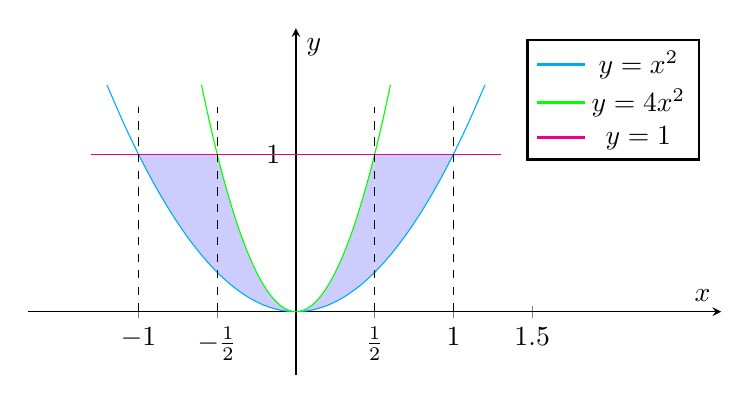
\begin{tikzpicture}
	\begin{axis}[
	legend pos=south east,
	y=2cm, x=2cm,
	xlabel={$x$}, ylabel={$y$},
	xmin=-1.7, xmax=2.7,
	ymin=-0.4, ymax=1.8,
	xtick={-1,-0.5,0,0.5,1,1.5}, 
	ytick={0,1},
	xticklabels={$-1$,$-\frac{1}{2}$,0,$\frac{1}{2}$,1,1.5}, yticklabels={0,1},
	line width=1pt,
	axis lines=center,
	legend pos=north east]
	legend style={at={(0.8,0.63)},anchor=north west},
	nodes near coords%,enlargelimits=0.2
	]
	\addplot[smooth,cyan,domain=-1.2:1.2,name path={A}] {x^2};%magenta品红
	\addplot[smooth,green,domain=-0.6:0.6,name path={B}] {4*x^2};
	\addplot[smooth,magenta,domain=-1.3:1.3,name path={C}] {1};
	\legend{$y = x^2$,$y=4x^2$,$y= 1$}
	\addplot[blue!20] fill between[of=A and B,soft clip={domain=-0.5:0.5}];
	\addplot[blue!20] fill between[of=A and C,soft clip={domain=-1:-0.5}];
	\addplot[blue!20] fill between[of=A and C,soft clip={domain=0.5:1}];
	\addplot[style=dashed,smooth,black,name path={S0}] coordinates{(-0.5,0)(-0.5,1.3)};
	\addplot[style=dashed,smooth,black,name path={S1}] coordinates{(0.5,0)(0.5,1.3)};
	\addplot[style=dashed,smooth,black,name path={S3}] coordinates{(-1,0)(-1,1.3)};
	\addplot[style=dashed,smooth,black,name path={S4}] coordinates{(1,0)(1,1.3)};
	\end{axis}\end{tikzpicture}\end{flushright}\hspace{5cm}\end{Solution}

\begin{Solution} \begin{align*}\iint\limits_{D}(x+y)\,\mathrm{d}\sigma&=\int_{0}^{1}\mathrm{d}y\!\int_{-\sqrt{y}}^{-\frac{\sqrt{y}}{2}}(x+y)\,\mathrm{d}x+\int_{0}^{1}\mathrm{d}y\!\int_{\frac{\sqrt{y}}{2}}^{\sqrt{y}}(x+y)\,\mathrm{d}x\\
&=\int_{0}^{1}\biggl[\frac{1}{2}x^2+xy\biggl]_{-\sqrt{y}}^{-\frac{\sqrt{y}}{2}}\mathrm{d}y+\int_{0}^{1}\biggl[\frac{1}{2}x^2+xy\biggl]_{\frac{\sqrt{y}}{2}}^{\sqrt{y}}\mathrm{d}y\\
&=\int_{0}^{1}\left(\frac{1}{2}y^{\frac{3}{2}}-\frac{3}{8}y\right)\mathrm{d}y+\int_{0}^{1}\left(\frac{1}{2}y^{\frac{3}{2}}+\frac{3}{8}y\right)\mathrm{d}y\\
&=\int_{0}^{1}y^{\frac{3}{2}}\mathrm{d}y=\biggl[\frac{2}{5}y^{\frac{5}{2}}\biggl]_{0}^{1}=\frac{2}{5}\\
\end{align*}
\end{Solution}

\begin{exercise}
计算二重积分 $\iint\limits_{x^2+y^2\leqslant R^2}e^x\cos y\dif x\dif y$.
\end{exercise}\begin{Solution}
令\[f(r)=\int_0^{2\pi}e^{r\cos\theta}\cos(r\sin\theta)d\theta,0\leqslant r\leqslant R,\]
则施行极坐标变换后得到
\[\iint\limits_{x^2+y^2\leqslant R^2}e^x\cos y\dif x\dif y=\int_0^Rrf(r)dr.\]
先证\[f(r)\equiv f(0)=2\pi.\]
事实上,\begin{align*}
f'(r)&=\int_0^{2\pi}e^{r\cos\theta}[\cos\theta \cos(r\sin\theta) -\sin\theta \sin (r\sin\theta)]d\theta\\
&=\frac{1}{r}\left(e^{r\cos\theta}\sin(r\sin\theta)\right)\Big|_0^{2\pi}\equiv 0.
\end{align*}
故 $f(r)\equiv f(0)=2\pi$. 因此
\[\iint\limits_{x^2+y^2\leqslant R^2}e^x\cos y\dif x\dif y=\int_0^Rrf(r)dr=\int_0^R2\pi rdr=\pi R^2.\]
\end{Solution}\begin{Solution}
由于\[\iint\limits_{x^2+y^2\leqslant R^2}e^x\sin y\dif x\dif y=\int_{-R}^Re^x\dif x\int_{-\sqrt{R^2-x^2}}^{\sqrt{R^2-x^2}}\sin y\dif y=0,\]
故\[\begin{split}\iint\limits_{x^2+y^2\leqslant R^2}e^x\cos y\dif x\dif y&=\iint\limits_{x^2+y^2\leqslant R^2}e^x(\cos y+i\sin 
y)\dif x\dif y\\ 
&=\iint\limits_{x^2+y^2\leqslant R^2}e^{x+iy}\dif x\dif y\\ 
&=\sum_{n=0}^\infty\frac{1}{n!}\iint\limits_{x^2+y^2\leqslant 
	R^2}(x+iy)^n\dif x\dif y\\ 
&=\sum_{n=0}^\infty\frac{1}{n!}\int_0^R 
r^{n+1}dr\int_0^{2\pi}e^{in\theta}d\theta\\ 
&=\int_0^R2\pi rdr\\ 
&=\pi R^2,\end{split}\]
其中用到极坐标变换, 函数项级数一致收敛从而可以逐项积分和如下事实:
\[\int_0^{2\pi}e^{in\theta}d\theta=\int_0^{2\pi}(\cos n\theta +i\sin n\theta)d\theta=\begin{cases}2\pi,&n=0,\\ 
0,& n\geqslant 1.\end{cases}\]
\end{Solution}

\section{特殊函数}

\begin{newthem}
设~$\displaystyle \varphi(n)$~是欧拉函数,且~$f$~是连续函数,求证\[\lim_{n\to+\infty}\frac{1}{n^2}\sum_{k=1}^{n}f\left(\frac{k}{n}\right)\varphi(k)=\frac{6}{{\pi}^2}\int_{0}^{1}xf(x)\dif x\]
实际上这个结果利用~\[\lim_{n\to+\infty}\frac{1}{n^2}\sum_{k=1}^{n}\varphi(k)=\frac{3}{{\pi}^2}~\mbox{和}~
\lim_{n\to+\infty}\frac{1}{n^\alpha}\sum_{k=1}^{n}f\left(\frac{k}{n}\right)a_{k}=A\int_{0}^{1}ax^{a-1}f(x)\dif x\]
其中~$\displaystyle A=\lim_{n\to+\infty}\sum_{k=1}^{n}\frac{a_{k}}{n},a_i>0,a>0$~拼一起	
\end{newthem}

\begin{exercise}求极限 $\lim_{s \to 0^+} \zeta(s)$
\end{exercise}\begin{Solution}
\begin{align*}
\zeta(0) & =\lim_{s \to 0^+} \zeta(s) \\
& =\lim_{s \to 0^+} 2^s \pi^{s-1} \sin \frac{\pi s}{2} \Gamma(1-s) \zeta(1-s) \\
& =\lim_{s \to 0^+} 2^s \pi^{s-1} \left( \sum_{n=0}^{\infty} \frac{(-1)^n}{(2n+1)!} \left( \frac{\pi s}{2} \right)^{2n+1} \right) \Gamma(1-s) \left( \frac{1}{(1-s)-1}+1-(1-s) \int_1^{\infty} \frac{x-[x]}{x^{(1-s)+1}} \, \dif x \right) \\
& =\lim_{s \to 0^+} 2^s \pi^{s-1} \left( \frac{\pi s}{2} \right) \left( \sum_{n=0}^{\infty} \frac{(-1)^n}{(2n+1)!} \left( \frac{\pi s}{2} \right)^{2n} \right) \Gamma(1-s) \left( \frac{1}{-s}+1-(1-s) \int_1^{\infty} \frac{x-[x]}{x^{2-s}} \, \dif x \right) \\
& =\lim_{s \to 0^+} 2^s \pi^{s-1} \left( \frac{\pi}{2} \right) \left( 1+\sum_{n=1}^{\infty} \frac{(-1)^n}{(2n+1)!} \left( \frac{\pi s}{2} \right)^{2n} \right) \Gamma(1-s) s \left( \frac{-1}{s}+1-(1-s) \int_1^{\infty} \frac{x-[x]}{x^{2-s}} \, \dif x \right) \\
& =\lim_{s \to 0^+} 2^{s-1} \pi^s \left( 1+\sum_{n=1}^{\infty} \frac{(-1)^n}{(2n+1)!} \left( \frac{\pi s}{2} \right)^{2n} \right) \Gamma(1-s) \left( -1+s-s(1-s) \int_1^{\infty} \frac{x-[x]}{x^{2-s}} \, \dif x \right) \\
& =\left( \lim_{s \to 0^+} 2^{s-1} \pi^s \Gamma(1-s) \left( -1+s-s(1-s) \int_1^{\infty} \frac{x-[x]}{x^{2-s}} \, \dif x \right) \right) \left( \lim_{s \to 0^+} 1+\sum_{n=1}^{\infty} \frac{(-1)^n}{(2n+1)!} \left( \frac{\pi s}{2} \right)^{2n} \right) \\
& =\left( 2^{0-1} \pi^0 \Gamma(1-0) \left( -1+0-0(1-0) \int_1^{\infty} \frac{x-[x]}{x^{2-0}} \, \dif x \right) \right) \left(1+\sum_{n=1}^{\infty} \frac{(-1)^n}{(2n+1)!} \left( \frac{\pi \cdot 0}{2} \right)^{2n} \right) \\
& =\left( \frac{1}{2} \cdot 1 \cdot \Gamma(1) \cdot (-1+0-0) \right) \left( 1+\sum_{n=1}^{\infty} 0 \right) \\
& =\frac{-1}{2}
\end{align*}	
\end{Solution}

\begin{example}
计算积分:~$\displaystyle\int_{\rm{0}}^{\rm{1}} \ln (1 - x)\ln x\ln (1 + x) \textrm{d}x$
\end{example}\begin{Solution}
\begin{align*}
I=&\int_{\rm{0}}^{\rm{1}} {\ln (1 - x)\ln x\ln (1 + x)\dif x} \\
=& \int_{\rm{0}}^{\rm{1}} {\ln (1 - x)\ln (1 + x)d(x\ln x - x + 1)} \\
=& \int_{\rm{0}}^{\rm{1}} {(x\ln x - x + 1)\left[ {\frac{{\ln (1 + x)}}{{1 - x}} - \frac{{\ln (1 - x)}}{{1 + x}}} \right]} \dif x\\
=& 2\int_{\rm{0}}^{\rm{1}} {(x\ln x - x + 1)\left[ {\sum\limits_{n = 0}^\infty  {({H_{2n + 1}} - {H_n}){x^{2n + 1}}} } \right]} \dif x\hspace{10mm}({H_0} = 0)\\
=& 2\sum\limits_{n = 0}^\infty  {({H_{2n + 1}} - {H_n})\int_0^1 {(x\ln x - x + 1){x^{2n + 1}}\dif x} } \\
=& 2\sum\limits_{n = 0}^\infty  {\frac{{{H_{2n + 1}} - {H_n}}}{{(2n + 3)(2n + 2)}}}  - 2\sum\limits_{n = 0}^\infty  {\frac{{{H_{2n + 1}} - {H_n}}}{{{{(2n + 3)}^2}}}} \\
=& \frac{{{\pi ^2}}}{6} - {\ln ^2}2 - 2 + 2\ln 2 - 2\left[ {\frac{{7\zeta (3)}}{{16}} + 2 - \ln 2 - \frac{{{\pi ^2}}}{8} - \sum\limits_{n = 1}^\infty  {\frac{{{H_n}}}{{{{(2n + 1)}^2}}}} } \right]\\
=& \frac{{5{\pi ^2}}}{{12}} - {\ln ^2}2 - 6 + 4\ln 2 + \frac{{21\zeta (3)}}{8} - \frac{{{\pi ^2}\ln 2}}{2}
\end{align*}
\end{Solution}\begin{note}
\[2\sum_{k=1}^{\infty}\frac{H_k}{(k+1)^m}=m\zeta(m+1)-\sum_{k=1}^{m-2}\zeta(m-k)\zeta(k+1)\]
\end{note}

\begin{exercise}计算积分\[I=\int_0^1 \ln (1 + x)\ln (1 - x) \textrm{d}x\]\end{exercise}\begin{Solution}因为\[\ln (1 + x)\ln (1 - x) = \sum\limits_{n = 1}^\infty  {\frac{{{H_n} - {H_{2n}} - \frac{1}{{2n}}}}{n}{x^{2n}}} \]
所以\[\int_0^1 {\ln (1 + x)\ln (1 - x)} \dif x = \sum\limits_{n = 1}^\infty  {\frac{{{H_n} - {H_{2n}}}}{{n(2n + 1)}}}  - \frac{1}{2}\sum\limits_{n = 1}^\infty  {\frac{1}{{{n^2}(2n + 1)}}} \]
Since\begin{align*}
I &= \int_0^1 {\ln (2 - x)\ln x} \dif x\\
& =  - \int_0^1 {x[\frac{{\ln (2 - x)}}{x} - \frac{{\ln x}}{{2 - x}}]} \dif x\\
&= 1 - 2\ln 2 + \int_0^1 {\frac{{x\ln x}}{{2 - x}}} \dif x\\
& = 1 - 2\ln 2 + 2\int_0^{\frac{1}{2}} {\frac{{(2x)\ln (2x)}}{{2 - 2x}}} \dif x\\
& = 1 - 3\ln 2 + 2{\ln ^2}2 + 2\int_0^{\frac{1}{2}} {\frac{{x\ln x}}{{1 - x}}} \dif x\\
&= 1 - 3\ln 2 + 2{\ln ^2}2 + 2\sum\limits_{k = 0}^\infty  {\int_0^{\frac{1}{2}} {{x^{k + 1}}\ln x} } \dif x\\
&= 1 - 3\ln 2 + 2{\ln ^2}2 - \sum\limits_{k = 0}^\infty  {\frac{{\ln 2}}{{(k + 2){2^{k + 1}}}} + \frac{1}{{{{(k + 2)}^2}{2^{k + 1}}}}} \dif x\\
&= 1 - 3\ln 2 + 2{\ln ^2}2 - \ln 2[2\ln 2 - 1] - \frac{{{\pi ^2}}}{6} + {\ln ^2}2 + 1\hspace{10mm}{\rm{        The~ value~ of ~ L}}{{\rm{i}}_2}(\frac{1}{2})\\
& = 2 - \frac{{{\pi ^2}}}{6} - 2\ln 2 + {\ln ^2}2
\end{align*}
and \[\sum\limits_{n = 1}^\infty  {\frac{1}{{{n^2}(2n + 1)}}}  = \frac{{{\pi ^2}}}{6} + 4\ln 2 - 4\]
所以\[\sum\limits_{n = 1}^\infty  {\frac{{{H_{2n}} - {H_n}}}{{n(2n + 1)}}}  = \frac{{{\pi ^2}}}{{12}} - {\ln ^2}2\]\end{Solution}		

\begin{exercise}计算积分:\[\int_{0}^{1}\frac{\ln^2(1-x)\ln x}{x}\dif x\]
\end{exercise}\begin{Solution}方法1
\begin{align*}
\int_{0}^{1}\frac{\ln^2(1-x)\ln x}{x}\dif x=&\int_{0}^{1}\ln(1-x)\ln xd\textrm{Li}_2(x)\\
=&\int_{0}^{1}\textrm{Li}_2(x)\frac{\ln(1-x)}{x}\dif x-\int_{0}^{1}\textrm{Li}_2(x)\frac{\ln x}{1-x}\dif x\\
=&-\frac{1}{2}\textrm{Li}_{2}^{2}(1)-\int_{0}^{1}\frac{\ln x}{1-x}\sum_{n=1}^{\infty}\frac{x^n}{n^2}\dif x\\
=&-\frac{1}{2}\textrm{Li}_{2}^{2}(1)+\sum_{n=1}^{\infty}\frac{1}{n^2}\sum_{k=n+1}^{\infty}\frac{1}{k^2}\\
=&-\frac{{\pi}^4}{72}+\frac{{\pi}^4}{120}=-\frac{{\pi}^4}{180}
\end{align*}
方法2
\begin{align*}
\int_{0}^{1}\frac{\ln^2(1-x)\ln x}{x}\dif x&=\frac{1}{2}\ln^2x\ln^2(1-x)\biggl|_{0}^{1}+\int_{0}^{1}\frac{\ln^2x\ln(1-x)}{1-x}\dif x\\
&=\int_{0}^{1}\sum_{k=1}^{\infty}(-1)^{2k-1}H_kx^k\ln^2x\dif x=\sum_{k=1}^{\infty}(-1)^{2k-1}H_k\int_{0}^{1}x^k\ln^2x\dif x\\
&=2\sum_{k=1}^{\infty}(-1)^{2k-1}\frac{H_k}{(k+1)^3}\\
&=2\sum_{k=1}^{\infty}(-1)^{2k-1}\left[\frac{H_{k+1}}{(k+1)^3}-\frac{1}{(k+1)^4}\right]\\
&=2\sum_{k=1}^{\infty}(-1)^{2k-1}\left[\frac{H_{k}}{k^3}-\frac{1}{k^4}\right]\\
&=-\frac{{\pi}^4}{36}+\frac{{\pi}^4}{45}=-\frac{{\pi}^4}{180}
\end{align*}	
\end{Solution}

\newpage\begin{exercise}计算积分\[\int_{0}^{1}{\frac{\ln{x}}{x^2-x-1}\dif x}\]
\end{exercise}\begin{Solution}由方程$x^2-x-1=0$的两个根,为了简单起见,我们记\\
$r_{1}=\varphi=\dfrac{1+\sqrt{5}}{2},r_{2}=\dfrac{1-\sqrt{5}}{2}=1-\varphi$,\\
且$r_{1}-r_{2}=\sqrt{5},\varphi^{2}=\varphi+1 , \dfrac{\varphi-1}{\varphi}=\dfrac{1}{\varphi^{2}}$
则有
\begin{align*} 
I&=\int_{0}^{1}{\frac{\ln{x}}{x^2-x-1}\dif x}=\frac{1}{r_{1}-r_{2}}\int_{0}^{1}{\ln{x}\left(\frac{1}{x-\varphi}-\frac{1}{x-(1-\varphi)} \right)\dif x}\\ 
&=\dfrac{1}{\sqrt{5}}\int_{0}^{1}{\ln{x}\left(\frac{1}{x-\varphi}-\frac{\varphi}{\varphi x+1}\right)\dif x}=\dfrac{1}{\sqrt{5}}\int_{0}^{1}{\frac{\ln{x}}{x-\varphi}\dif x}-\frac{\varphi}{\sqrt{5}}\int_{0}^{1}{\frac{\ln{y}}{\varphi y+1}\dif y}\\ 
&=\frac{1}{\sqrt{5}}\int_{0}^{\frac{1}{\varphi}}{\frac{\ln{\varphi u}}{u-1}\dif u}-\frac{1}{\sqrt{5}}\int_{0}^{\varphi}{\frac{\ln{\frac{u}{\varphi}}}{u+1}\dif u}\\ 
&=\frac{\ln{\varphi}}{\sqrt{5}}\left(\int_{0}^{\frac{1}{\varphi}}{\frac{1}{u-1}\dif u}+\int_{0}^{\varphi}{\frac{1}{u+1}\dif u} \right)-\frac{1}{\sqrt{5}}\left(\int_{0}^{\varphi}{\frac{\ln{u}}{1+u}\dif u}+\int_{0}^{\frac{1}{\varphi}}{\frac{\ln{u}}{1-u}\dif u} \right)\\ 
&=\frac{\ln{\varphi}}{\sqrt{5}}\ln{\frac{\varphi^{2}-1}{\varphi}}-\frac{1}{\sqrt{5}}\left(\int_{0}^{\varphi}{\frac{\ln{u}}{1+u}\dif u}+\int_{0}^{\frac{1}{\varphi}}{\frac{\ln{u}}{1-u}\dif u} \right)\\ 
&=-\frac{1}{\sqrt{5}}\left(\int_{0}^{\varphi}{\frac{\ln{u}}{1+u}\dif u}+\int_{0}^{\frac{1}{\varphi}}{\frac{\ln{u}}{1-u}\dif u} \right)=-\frac{1}{\sqrt{5}}\left(\int_{1}^{1+\varphi}{\frac{\ln{(u-1)}}{u}\dif u}+\int_{0}^{\frac{1}{\varphi}}{\frac{\ln{u}}{1-u}\dif u}  \right)\\ 
&=-\frac{1}{\sqrt{5}}\left(\int_{1}^{\varphi^{2}}{\frac{\ln{(u-1)}}{u}\dif u}+\int_{0}^{\frac{1}{\varphi}}{\frac{\ln{u}}{1-u}\dif u}  \right)\\ 
&=-\frac{1}{\sqrt{5}}\left(\int_{\frac{1}{\varphi^{2}}}^{1}{\frac{\ln{(1-u)}-\ln{u}}{u}\dif u}+\int_{0}^{\frac{1}{\varphi}}{\frac{\ln{u}}{1-u}\dif u}  \right)\\ 
&=-\frac{1}{\sqrt{5}}\left(\int_{0}^{\frac{1}{\varphi}}{\frac{\ln{u}-\ln{(1-u)}}{u}\dif u}+\int_{0}^{\frac{1}{\varphi}}{\frac{\ln{u}}{1-u}\dif u}  \right)\\ 
&=-\frac{2}{\sqrt{5}}\int_{0}^{\frac{1}{\varphi}}{\frac{\ln{u}}{1-u}\dif u}+\frac{1}{\sqrt{5}}\int_{0}^{\frac{1}{\varphi}}{\frac{\ln{(1-u)}}{1-u}\dif u}\\ 
&=-\frac{2}{\sqrt{5}}\int_{0}^{\frac{1}{\varphi}}{\frac{\ln{u}}{1-u}\dif u}-\frac{2}{\sqrt{5}}\ln^{2}{\varphi}=-\frac{2}{\sqrt{5}}\int_{\frac{1}{\varphi^{2}}}^{1}{\frac{\ln{(1-u)}}{u}\dif u}-\frac{2}{\sqrt{5}}\ln^{2}{\varphi}\\ 
&=-\frac{2}{\sqrt{5}}\left(\int_{0}^{1}{\frac{\ln{(1-u)}}{u}\dif u}-\int_{0}^{\frac{1}{\varphi^{2}}}{\frac{\ln{(1-u)}}{u}\dif u} \right)-\frac{2}{\sqrt{5}}\ln^{2}{\varphi}\\ 
&=\frac{\pi^{2}}{3\sqrt{5}}-\frac{2}{\sqrt{5}}\mathrm{Li\,}_{2}{\left(\frac{1}{\varphi^{2}}\right)}-\frac{2}{\sqrt{5}}\ln^{2}{\varphi}\\
&=\frac{\pi^{2}}{3\sqrt{5}}-\frac{2}{\sqrt{5}}\left(\frac{\pi^{2}}{15}-\ln^{2}{\varphi} 
\right)-\frac{2}{\sqrt{5}}\ln^{2}{\varphi}=\frac{\pi^{2}}{5\sqrt{5}} 
\end{align*}
最后一步用了dilogarithm函数的性质,详细可以参见http://mathworld.wolfram.com/Dilogarithm.html	
\end{Solution}

\begin{example}
求定积分 \[\int_0^1\frac{\ln^2(1+x^2)}{1+x^2}\dif x\]
\end{example}\begin{Solution}(by Renascence\verb|_|5)
\begin{align*}
&\int_0^1\frac{\ln^2(1+x^2)}{1+x^2}\dif x\\
=&\int_0^1\frac{\ln^2(1-y^2)}{1+\mathrm{i}y}\mathrm{i}\dif y-\int_0^{\frac{\pi}{2}}\frac{\ln^2(1+e^{\mathrm{i}2\theta})}{1+e^{\mathrm{i}\theta}}\dif\theta\\
=&\underbrace{\int_0^1\frac{y\ln^2(1-y^2)}{1+y^2}\dif y}_{I_1}+\underbrace{\frac{1}{2}\int_0^{\frac{\pi}{2}}\tan\left(\frac{\theta}{2}\right)\ln^2(2\cos\theta)\dif\theta}_{I_2}+\underbrace{\int_0^{\frac{\pi}{2}}\theta\ln(2\cos\theta)\dif\theta}_{I_3}-\underbrace{\frac{1}{2}\int_0^{\frac{\pi}{2}}\theta^2\tan\left(\frac{\theta}{2}\right)\dif\theta}_{I_4}
\end{align*}
\textbf{Evaluation of} $I_1$:
\begin{align*}
I_1&=\frac{1}{2}\int_0^1\frac{\ln^2(1-y)}{1+y}\dif y=\frac{1}{4}\int_0^1\frac{\ln^2y}{1-y/2}\dif y\\
&=\frac{1}{4}\sum_{n=0}^{\infty}\frac{1}{2^n}\int_0^1y^2\ln^2y\dif y=\sum_{n=0}^{\infty}\frac{1}{2^{n+1}(n+1)^3}\\
&=\Li_3\left(\frac{1}{2}\right)=\frac{7}{8}\zeta(3)-\frac{\pi^2}{12}\ln2+\frac{1}{6}\ln^32
\end{align*}
\textbf{Evaluation of} $I_2$:
\begin{align*}
I_2&=\int_0^1\frac{x}{1+x^2}\ln^2\left(2\frac{1-x^2}{1+x^2}\right)\dif x\\
&=\frac{1}{2}\int_0^1\frac{1}{1+x}\ln^2\left(2\frac{1-x}{1+x}\right)\dif x\\
&=\frac{1}{2}\int_0^1\frac{\ln^2x}{1+x}\dif x+\ln2\int_0^1\frac{\ln x}{1+x}\dif x+\frac{1}{2}\ln^22\int_0^1\frac{1}{1+x}\dif x\\
&=\frac{1}{2}\sum_{n=0}^{\infty}(-1)^n\int_0^1x^n\ln^2x\dif x+\ln2\sum_{n=0}^{\infty}(-1)^n\int_0^1x^n\ln x\dif x+\frac{1}{2}\ln^32\\
&=\sum_{n=0}^{\infty}\frac{(-1)^n}{(n+1)^3}-\ln2\sum_{n=0}^{\infty}\frac{(-1)^n}{(n+1)^2}+\frac{1}{2}\ln^32\\
&=\frac{3}{4}\zeta(3)-\frac{\pi^2}{12}\ln2+\frac{1}{2}\ln^32
\end{align*}
\textbf{Evaluation of} $I_3$:
\begin{align*}
I_3&=\sum_{n=1}^{\infty}\frac{(-1)^{n-1}}{n}\int_0^{\frac{\pi}{2}}\theta\cos(2n\theta)\dif\theta\\
&=-\frac{1}{4}\sum_{n=1}^{\infty}\frac{1}{n^3}-\frac{1}{4}\sum_{n=1}^{\infty}\frac{(-1)^{n-1}}{n^3}\\
&=-\frac{7}{16}\zeta(3)
\end{align*}
\textbf{Evaluation of} $I_4$:
\begin{align*}
I_4&=\left[\theta^2\ln\left(\cos\frac{\theta}{2}\right)\right]_0^{\frac{\pi}{2}}-2\int_0^{\frac{\pi}{2}}\theta\ln\left(\cos\frac{\theta}{2}\right)\dif\theta\\\
&=-\frac{\pi^2}{8}\ln2+2\ln2\int_0^{\frac{\pi}{2}}\theta\dif\theta-2\sum_{n=1}^{\infty}\frac{(-1)^{n-1}}{n}\int_0^{\frac{\pi}{2}}\theta\cos(n\theta)\dif\theta\\
&=\frac{\pi^2}{8}\ln2+2\sum_{n=1}^{\infty}\frac{(-1)^{n-1}}{n^3}-\pi\sum_{n=1}^{\infty}\frac{(-1)^{n-1}\sin(n\pi/2)}{n^2}-2\sum_{n=1}^{\infty}\frac{(-1)^{n-1}\cos(n\pi/2)}{n^2}\\
&=\frac{21}{16}\zeta(3)-\pi\mathrm{\mathbf{G}}+\frac{\pi^2}{8}\ln2
\end{align*}
\textbf{Result}:
\begin{align*}
\color{blue}\int_0^1\frac{\ln^2(1+x^2)}{1+x^2}\dif x
&=\left(\frac{7}{8}+\frac{3}{4}-\frac{7}{16}+\frac{21}{16}\right)\zeta(3)-\pi\mathrm{\mathbf{G}}+\left(-\frac{\pi^2}{12}-\frac{\pi^2}{12}+\frac{\pi^2}{8}\right)\ln2+\left(\frac{1}{6}+\frac{1}{2}\right)\ln^32\\
&=\color{blue}\frac{5}{2}\zeta(3)-\pi\mathrm{\mathbf{G}}-\frac{\pi^2}{24}\ln2+\frac{2}{3}\ln^32
\end{align*}
\end{Solution}

\begin{exercise}
计算积分:\[\int_{0}^{1}\frac{\ln^2(1-x)\ln x}{x}\dif x\]
\end{exercise}\begin{solution}
\begin{equation*}\begin{aligned}
\int_{0}^{1}\frac{\ln^2(1-x)\ln x}{x}\dif x=&\int_{0}^{1}\ln(1-x)\ln xd\textrm{Li}_2(x)\\
=&\int_{0}^{1}\textrm{Li}_2(x)\frac{\ln(1-x)}{x}\dif x-\int_{0}^{1}\textrm{Li}_2(x)\frac{\ln x}{1-x}\dif x\\
=&-\frac{1}{2}\textrm{Li}_{2}^{2}(1)-\int_{0}^{1}\frac{\ln x}{1-x}\sum_{n=1}^{\infty}\frac{x^n}{n^2}\dif x\\
=&-\frac{1}{2}\textrm{Li}_{2}^{2}(1)+\sum_{n=1}^{\infty}\frac{1}{n^2}\sum_{k=n+1}^{\infty}\frac{1}{k^2}\\
=&-\frac{{\pi}^4}{72}+\frac{{\pi}^4}{120}=-\frac{{\pi}^4}{180}
\end{aligned}\end{equation*}
\end{solution}

\begin{theorem}{华里士公式}{}
\begin{align*}
I_n&=\int_0^{\frac{\pi}{2}}\sin^nx\,\mathrm{d}x=\int_0^{\frac{\pi}{2}}\cos^nx\,\mathrm{d}x\\
&=\begin{cases}
\displaystyle\frac{n-1}{n}\cdot\frac{n-3}{n-2}\cdot\,\cdots\,\cdot\frac{3}{4}\cdot \frac{1}{2}\cdot\frac{\pi}{2},&\quad n\mbox{为正偶数},~I_0=\frac{\pi}{2}\\[4mm]
\displaystyle\frac{n-1}{n}\cdot\frac{n-3}{n-2}\cdot\,\cdots\,\cdot\frac{4}{5}\cdot \frac{2}{3},&\hspace{0.4cm}n \mbox{为大于1 的正奇数},~I_1=1
\end{cases}
\end{align*}	
\end{theorem}\begin{proof}
首先, 作代换 $x=t+\dfrac{\pi}{2}$, 由换元积分法得
$$I_n=\int_0^{\frac{\pi}{2}}\sin^n x\dif x=\int_{-\frac{\pi}{2}}^{0}\cos^n t\dif t=-\int_{\frac{\pi}{2}}^0\cos^n t\dif t=\displaystyle\int_0^{\frac{\pi}{2}}\cos^n x\dif x.$$
其次,
\begin{align*}
I_n&=\int_0^{\frac{\pi}{2}}\sin^{n-1} x \dif (-\cos x)\\
&=[-\cos x \sin^{n-1} x]_0^{\frac{\pi}{2}}+\int_0^{\frac{\pi}{2}}{\cos x}\dif (\sin^{n-1}x)\\
&=(n-1)\int_0^{\frac{\pi}{2}}{\cos^2 x \sin^{n-2} x}\dif x\\
&=(n-1)\int_0^{\frac{\pi}{2}}(1-\sin^2 x) \sin^{n-2} x\dif x\\
&=(n-1)\int_0^{\frac{\pi}{2}}{\sin^{n-2} x}{\rm d}x-(n-1)\int_0^{\frac{\pi}{2}}{\sin^{n} x}\dif x\\
&=(n-1)I_{n-2}-(n-1)I_n,	
\end{align*}
从而得递推公式 $$I_n=\dfrac{n-1}{n}I_{n-2}.$$ 注意到
$$I_0=\int_0^{\frac{\pi}{2}}\sin^0 x\dif x=\dfrac{\pi}{2},\quad I_1=\int_0^{\frac{\pi}{2}}\sin x \dif x=1,$$
当 $n$ 为偶数时,
\begin{align*}
I_{n}&=\frac{n-1}{n}I_{n-2}=\frac{n-1}{n}\cdot\frac{n-3}{n-2}I_{n-4}=\cdots \\
&= \frac{n-1}{n}\cdot\frac{n-3}{n-2}\cdots\frac{3}{4}\cdot\frac{1}{2}\cdot I_0= \frac{n-1}{n}\cdot\frac{n-3}{n-2}\cdots\frac{3}{4}\cdot\frac{1}{2}\cdot\frac{\pi}{2},	
\end{align*}
而当 $n$ 为奇数时,
\begin{align*}
I_{n}&=\frac{n-1}{n}I_{n-2}=\frac{n-1}{n}\cdot\frac{n-3}{n-2}I_{n-4}=\cdots \\
&= \frac{n-1}{n}\cdot\frac{n-3}{n-2}\cdots\frac{4}{5}\cdot\frac{2}{3}\cdot I_1= \frac{n-1}{n}\cdot\frac{n-3}{n-2}\cdots\frac{4}{5}\cdot\frac{2}{3},	
\end{align*} 结论获证.
\end{proof}

\section{积分不等式}

\begin{example}
证明\[\int_0^{\frac{\pi}{2}}\big(e^{\sin x}-e^{-\cos x}\big)\dif x\geqslant2\]
\end{example}\begin{newproof}
\[e^{\sin x}=1+\sin x+\frac{\sin^2x}{2!}+\cdots\]
\[e^{-\sin x}=1-\sin x+\frac{\sin^2x}{2!}+\cdots\]
所以\[e^{\sin x}-e^{-\sin x}=2\sin x+2\cdot\frac{\sin^3x}{3!}+\cdots\geqslant2\sin x\]
因此
\begin{align*}
\int_0^{\frac{\pi}{2}}\big(e^{\sin x}-e^{-\cos x}\big)\dif x
&=\int_0^{\frac{\pi}{2}}e^{\sin x}\dif x-\int_0^{\frac{\pi}{2}}e^{-\cos x}\dif x\\
&=\int_0^{\frac{\pi}{2}}e^{\sin x}\dif x-\int_0^{\frac{\pi}{2}}e^{-\sin x}\dif x\\
&=\int_0^{\frac{\pi}{2}}\big(e^{\sin x}-e^{-\sin x}\big)\dif x\\
&\geqslant\int_0^{\frac{\pi}{2}}2\sin x=2	
\end{align*}	
\end{newproof}

\begin{newthem}
若 $D=\{(x,y)|\varphi_1(x)\leqslant y\leqslant\varphi_2(x),a\leqslant x\leqslant b\}$, $\varphi_1(x)$, $\varphi_2(x)$ 连续 , 则 $D$ 的面积为\begin{equation*}S_D=\int_{a}^{b}\left[\varphi_2(x)-\varphi_1(x)\right]\,\mathrm{d}x\end{equation*}	
\end{newthem}

\begin{newthem}
若 $D=\{(x,y)|\psi_1(y)\leqslant x\leqslant\psi_2(y),c\leqslant y\leqslant d\}$, $\psi_1(y)$, $\psi_2(y)$  连续 , 则 $D$ 的面积为\begin{equation*}S_D=\int_{c}^{d}\left[\psi_2(y)-\psi_1(y)\right]\,\mathrm{d}y\end{equation*}	
\end{newthem}

\begin{example}
设 $f(x)$ 在 $[0,\pi]$ 上可微,若 $\int_0^\pi f(x)\dif x=0$,则
\[\int_0^\pi f^2(x)\dif x\leqslant\int_0^\pi\big[f'(x)\big]^2\dif x\]
\end{example}\begin{proof}
将 $f(x)$ 在 $[-\pi,\pi]$ 上作偶延拓,从而可展开成 Fourier 余弦级数
\[f(x)=\sum_{n=1}^{\infty}a_n\cos nx\quad(a_0=0)\]
此时,易知有 $f(-\pi)=f(\pi)$
\[f'(x)\sim\sum_{n=1}^{\infty}(-na_n)\sin nx\]
从而由 $a_n^2\leqslant(-na_n)^2\;(n=1,2,\cdots)$, 根据 Parseval 等式,我们有
\[\frac{1}{\pi}\int_0^\pi f^2(x)\dif x\leqslant\frac{1}{\pi}\int_0^\pi\big[f'(x)\big]^2\dif x\]
\end{proof}

\begin{example}\label{exam:intneq-amm11946}
(\href{https://www.mat.uniroma2.it/~tauraso/AMM/AMM11946.pdf}{AMM11946}) %设 $f(x)$ 在 $[0,1]$ 上二阶连续可微, 且 $\int_{\frac{1}{3}}^{\frac{2}{3}}f(x)\dif x=0$. 证明:\[4860\left(\int_0^1f(x)\dif x \right)^2\leqslant 11\int_0^1\big(f''(x)\big)^2\dif x \]
Let $f$ be a twice differentiable function [0,1] to $\mathbb R$ with $f''$ continuous on [0,1] and $\int_{\frac{1}{3}}^{\frac{2}{3}}f(x)\dif x=0$. Proof:
\[4860\left(\int_0^1f(x)\dif x \right)^2\leqslant 11\int_0^1\big(f''(x)\big)^2\dif x \]
\end{example}\begin{proof}
Let $g(x)$ be the piecewise differentiable function defined as
\[g(x):=\begin{cases}
x   & \text{if}\; x\in[0,1/3),\\
1-2x& \text{if}\; x\in[1/3,2/3],\\
x-1 & \text{if}\; x\in[2/3,1),
\end{cases}\]
and let
\[G(x):=\int_0^xg(t)\dif t=\begin{cases}
\frac{x^2}{2}   & \text{if}\; x\in[0,1/3),\\
-x^2+x-\frac{1}{6}& \text{if}\; x\in[1/3,2/3],\\
\frac{x^2}{2}-x+\frac{1}{2}& \text{if}\; x\in[2/3,1).
\end{cases}  \]
Since $\int_{\frac{1}{3}}^{\frac{2}{3}}f(x)\dif x=0$, it follows that
\[\int_0^1 f(x)\dif x=\int_0^{\frac{1}{3}} f(x)\dif x-2\int_{\frac{1}{3}}^{\frac{2}{3}} f(x)\dif x+\int_{\frac{2}{3}}^1 f(x)\dif x=\int_0^1 f(x)g'(x)\dif x. \]
Hence, by integrating by parts,we obtain
\begin{align*}
\int_0^1 f(x)\dif x&=\int_0^1 f(x)\dif(g(x))=\big[f(x)g(x)\big]_0^1-\int_0^1 g(x)\dif(f(x))=\int_0^1 g(x)f'(x)\dif x\\
&=-\int_0^1 f'(x)\dif(G(x))=-\big[f'(x)G(x)\big]_0^1+\int_0^1 f''(x)G(x)\dif x=\int_0^1 f''(x)G(x)\dif x
\end{align*}
Finally, by Cauchy-Schwarz inequality, we get
\[\left(\int_0^1 f(x)\dif x\right)^2\leqslant \int_0^1 \big(G(x)\big)^2\dif x\cdot\int_0^1 \big(f''(x)\big)^2\dif x=\frac{11}{4860}\int_0^1 \big(f''(x)\big)^2\dif x \]
because 
\[\int_0^1 \big(G(x)\big)^2\dif x=2\int_0^{\frac{1}{3}} \frac{x^4}{4}\dif x+2\int_{\frac{1}{3}}^{\frac{1}{2}}\left(-x^2+x-\frac{1}{6}\right)^2\dif x=\frac{11}{4860}.\]
\end{proof}

%\begin{newthem}
%若 $D=\{(\rho,\theta)|\rho_1(\theta)\leqslant \rho\leqslant\rho_2(\theta),\alpha\leqslant \theta\leqslant \beta\}$, $\rho_1(\theta)$, $\rho_2(\theta)$  连续 , 则 $D$ 的面积为\begin{equation*}S_D=\frac{1}{2}\int_{\alpha}^{\beta}\left[\rho_2^2(\theta)-\rho_1^2(\theta)\right]\,\mathrm{d}\theta\end{equation*}这里 $(\rho,\theta)$ 为极坐标。	
%\end{newthem}

%(2.1) 将由 $x$ 轴, 直线 $x=a$, $x=b$ \,$(a<b)$ , 及连续曲线 $y=f(x)\,(f(x)\geqslant0)$ 所围成的曲边梯形绕 $x$ 轴旋转一周所得到的旋转体的体积 \;\;$V_x=\pi\int_a^bf^2(x)\,\mathrm{d}x$

%(2.2) 将由 $y$ 轴, 直线 $y=c$, $y=d$ \,$(c<d)$ , 及连续曲线 $x=\varphi(y) \,(\varphi(y)\geqslant0)$ 所围成的曲边梯形绕 $y$ 轴旋转一周所得到的旋转体的体积 \;\;$V_y=\pi\int_c^d\varphi^2(y)\,\mathrm{d}y$

\chapter{重积分} %重积分

\begin{example}
证明不等式:
\[2\pi\left(\sqrt{17}-4\right)\le \iint\limits_{x^2+y^2\le 1}\frac{\text{d}x\text{d}y}{\sqrt{16+\sin^2x+\sin^2y}}\le \frac{\pi}{4}.\]	
\end{example}
\begin{solution}
左边不等式:\begin{align*}
\iint\limits_{{{x}^2}+{{y}^2}\leqslant 1}{\frac{\text{d}x\text{d}y}{\sqrt{16+{{\sin }^2}x+{{\sin }^2}y}}}&\geqslant \iint\limits_{{{x}^2}+{{y}^2}\leqslant 1}{\frac{\text{d}x\text{d}y}{\sqrt{16+x^2+y^2}}}\\
&=2\pi (16+r^2)^{1/2}\Big|_0^1= 2\pi \left( \sqrt{17}-4 \right).
\end{align*}
右边不等式:\[\iint\limits_{x^2+y^2\leqslant1}\frac{\dif x\dif y}{\sqrt{16+\sin^2x+\sin^2y}}\leqslant4\iint\limits_{x^2+y^2\leqslant1}\dif x\dif y=\frac{\pi}{4}\]
\end{solution}

\begin{exercise}
设二元函数 $f(x,y)$ 在区域
\[D=\big\{0\leqslant x\leqslant1,0\leqslant y\leqslant1\big\}\]
上具有连续的四阶偏导数, $f(x,y)$ 在 $D$ 的边界上恒为零, 且 $\bigg|\frac{\partial^4f}{\partial x^2\partial y^2}\bigg|\leqslant3$, 试证明
\[\bigg|\iint_Df(x,y)\dif x\dif y\bigg|\leqslant\frac{1}{48}\]
\end{exercise}\begin{proof}
法II(by xwmath)\footnote{考研竞赛数学:每日一题271:多元函数高阶偏导数条件的不等式证明}.
%\href{https://mp.weixin.qq.com/s?__biz=MzI2OTE2NzczNQ==&mid=2649990740&idx=2&sn=520ec6ed5986a63e663be85db0b05231&chksm=f2e37b4cc594f25a5a8c5307d80e46d777db949b8e3ace5dc29ebcca020addaa000675e65c9a&mpshare=1&scene=23&srcid=#rd}{考研竞赛数学:每日一题271:多元函数高阶偏导数条件的不等式证明}
由于 $f(x,y)$ 在 $D$ 的边界上恒为零, 所以
\begin{align*}
\int_0^1x(1-x)\frac{\partial^4 f}{\partial x^2\partial y^2}\dif x
&=\int_0^1x(1-x)\dif \frac{\partial^3f}{\partial x\partial y^2} \\
&=\left[\frac{\partial^3f}{\partial x \partial y^2} x(1-x)\right]_0^1-\int_0^1 \frac{\partial^3f}{\partial x \partial y^2}(1-2x)\dif x\\ 
&=\int_0^1(2 x-1)\dif \frac{\partial^3f}{\partial y^2}=\left[(2x-1) \frac{\partial^2f}{\partial y^2}\right]_0^1-2 \int_0^1\frac{\partial^2f}{\partial y^2}\dif x \\ 
&=-2\int_0^1\frac{\partial^2f}{\partial y^2}\dif x
\end{align*}
类似可得
\begin{align*}
\int_0^1y(1-y)\frac{\partial^2f}{\partial y^2}\dif  y&=\int_0^1y(1-y)\dif \frac{\partial f}{\partial y}\\
&=y(1-y)\left.\frac{\partial f}{\partial y}\bigg|_0 ^1-\int_0^1(1-2y)\frac{\partial f}{\partial y}\dif y\right.\\
&=\int_0^1(2y-1)\dif f(x, y) \\
&=[(2y-1)f(x,y)]_0^1-2\int_0^1f(x,y)\dif y \\
&=-2\int_0^1f(x,y)\dif y 
\end{align*}
将两个结果分别视为二重积分中的两个累次积分计算, 于是可得
\begin{align*} 
\iint_Dx(1-x)y(1-y)\frac{\partial^4f}{\partial x^2\partial y^2} \dif x\dif y 
&=-2\int_0^1\left[-2\int_0^1f(x,y)\dif y\right]\dif x \\
&=4\int_0^1\left[\int_0^1f(x,y)\dif y\right]\dif x=4\iint_Df(x,y)\dif x\dif y 
\end{align*}
于是由 $\bigg|\frac{\partial^4f}{\partial x^2\partial y^2}\bigg|\leqslant3$, 得
\begin{align*} 
\left|\iint_{D} f(x, y)\dif x\dif y\right|
&=\frac{1}{4}\left|\iint_{D} x y(1-x)(1-y)\frac{\partial^4 f}{\partial x^2\partial y^2}\dif x\dif y\right|\\ 
&\leqslant\frac{3}{4}\left|\iint_{D} x y(1-x)(1-y)\dif x\dif y\right| \\
&= \frac{3}{4}\left|\int_0^1 x(1-x)\dif x\int_0^1y(1-y)\dif y\right|\\
&=\frac{3}{4}\left|\int_0^1x(1-x)\dif x\int_0^1y(1-y)\dif y\right|\\
&=\frac{3}{4}\left(\int_0^1x(1-x)\dif x\right)^2=\frac{3}{4} \cdot \frac{1}{36}=\frac{1}{48}
\end{align*}
\end{proof}

\chapter{级数}

\section{无穷带来的各种悖论}
当时我就震惊了:无穷带来的各种悖论

\par 希尔伯特旅馆悖论(Hilbert's paradox of Grand Hotel): 希尔伯特旅馆有无限个房间, 并且每个房间都住了客人.一天来了一个新客人, 旅馆老板说:“虽然我们已经客满, 但你还是能住进来的. 我让 1 号房间的客人搬到 2 号房间, 2 号房间搬到 3 号房间 $n$ 号房间搬到 $n+1$ 号房间, 你就可以住进 1 号房间了.” 又一天, 来了无限个客人, 老板又说: “不用担心, 大家仍然都能住进来. 我让 1 号房间的客人搬到 2 号房间, 2 号搬到 4 号, 3 号搬到 6 号 $n$ 号搬到 $2n$ 号, 然后你们排好队, 依次住进奇数号的房间吧.”

\par 托里拆利小号(Torricelli‘s Horn): 意大利数学家托里拆利(Evangelista Torricelli)将 $y=1/x$ 中 $x\geqslant1$ 的部分绕着 $x$ 轴旋转了一圈, 得到了上面的小号状图形(注意, 上图只显示了这个图形的一部分). 然后他算出了这个小号的一个十分有趣的性质——它的表面积无穷大, 可它的体积却是 $\pi$. 这明显有悖于人的直觉: 体积有限的物体, 表面积却可以是无限的!换句话说, 填满整个托里拆利小号只需要有限的油漆, 但把托里拆利小号的表面刷一遍, 却需要无限多的油漆!

\par “科赫雪花”(Koch Snow flake): 科赫雪花是一种经过无穷多次迭代生成的分形图形, 下图就是前三次迭代的过程, 迭代过程的极限便是科赫雪花了. 它也有一个类似的性质:它的面积有限, 周长却是无限的. 用无限的周长包围了一块有限的面积, 真是另类的“无中生有”啊!

%\par 芝诺悖论(Zeno's paradox): 在芝诺(Zeno)五岁那年, 他父亲问他:“从我们家到外婆家一共有五公里的路要走, 如果你以每小时五公里速度去外婆家, 那你需要多长时间才能到?”芝诺回答道:“一小时.” 十年之后,芝诺十五岁, 他父亲又问了他一遍相同的问题. 你可能会说, 芝诺父亲怎么会这么无聊?但是芝诺却回答:“永远也走不到.” 芝诺是这样回答他父亲的:“如果将五公里的路程一分为二, 那如果想去外婆家就要先走过这段路程的前一半;再将剩下的一半路程一分为二, 如果想要到外婆家, 同样也要走剩下路程的前一半. 之后再将剩下的路程一分为二, 这样无论走久都到不了外婆家, 所以永远也走不到.” 这其实就是著名的芝诺悖论.

\par 阿基里斯与乌龟的悖论(Achilles and the tortoise Paradox): 在跑步比赛中, 如果跑得最慢的乌龟一开始领先跑得最快的希腊勇士阿基里斯, 那么乌龟永远也不会被阿基里斯追上. 因为要想追到乌龟, 阿基里斯必须先到达乌龟现在的位置; 而等阿基里斯到了这个位置之后乌龟已经又前进了一段距离. 如此下去, 阿基里斯永远追不上乌龟.

\par 二分法悖论(Dichotomy Paradox): 运动是不可能的. 你要到达终点, 必须首先到达全程的 1/2 处; 而要到达 1/2 处, 必须要先到 1/4 处⋯⋯每当你想到达一个点, 总有一个中点需要先到, 因此你是永远也到不了终点的. 其实,你根本连动都动不了, 运动是不可能的.

\begin{example}
设 ${a_n} = 1 + \frac{1}{2} + \cdots + \frac{1}{n},n = 1,2, \cdots$,求 $\sum\limits_{n = 1}^\infty {\frac{{{a_n}}}{{n\left( {n + 1} \right)}}}$ 的和.
\end{example}\begin{solution}
\begin{align*}
\sum\limits_{n = 1}^\infty {\frac{{{a_n}}}{{n\left( {n + 1} \right)}}} =& \sum\limits_{n = 1}^\infty {\frac{{1 + \frac{1}{2} + \cdots + \frac{1}{n}}}{{n\left( {n + 1} \right)}}} \\
=&\sum\limits_{n = 1}^\infty {\left( {\frac{{1 + \frac{1}{2} + \cdots + \frac{1}{n}}}{n} - \frac{{1 + \frac{1}{2} + \cdots + \frac{1}{{n + 1}}}}{{n + 1}}} \right)} + \sum\limits_{n = 1}^\infty {\frac{1}{{{{\left( {n + 1} \right)}^2}}}} \\
= & 1 - \mathop {\lim }\limits_{n \to \infty } \frac{{1 + \frac{1}{2} + \cdots + \frac{1}{{n + 1}}}}{{n + 1}} + \left( {\frac{{{\pi ^2}}}{6} - 1} \right) = \frac{{{\pi ^2}}}{6} - \mathop {\lim }\limits_{n \to \infty } \frac{{\frac{1}{{n + 2}}}}{1} \\
=& \frac{{{\pi ^2}}}{6}.
\end{align*}
\end{solution}

\begin{example}
求 $\sum_{n=1}^{\infty}\frac{1}{\sqrt{n(n+1)}(\sqrt{n}+\sqrt{n+1})}$ 的和	
\end{example}\begin{proof}
注意到
\[\frac{1}{\sqrt{n(n+1)} (\sqrt{n} + \sqrt{n+1})} = \frac{\sqrt{n+1} -\sqrt{n}}{\sqrt{n(n+1)}} = \frac1{\sqrt{n}} - \frac1{\sqrt{n+1}}\]
故\[\sum_{n=1}^{\infty}\frac{1}{\sqrt{n(n+1)} (\sqrt{n} + \sqrt{n+1})} 
=  \sum_{n=1}^{\infty}\left(\frac1{\sqrt{n}} - \frac1{\sqrt{n+1}}\right)=1\]
%\begin{align*}
%&\sum_{n=1}^{\infty}\frac{1}{\sqrt{n(n+1)} (\sqrt{n} + \sqrt{n+1})} 
%=  \sum_{n=1}^{\infty}\left(\frac1{\sqrt{n}} - \frac1{\sqrt{n+1}}\right)=1%\\
%=& \frac{1}{1}-\frac{1}{\sqrt{2}} + \frac{1}{\sqrt{2}} - \frac{1}{\sqrt{3}}+\cdots+\frac1{\sqrt{n}} - \frac1{\sqrt{n+1}}+\cdots = 1
%\end{align*}
\end{proof}

\begin{example}
计算 $\displaystyle \sum_{n=1}^\infty \arctan\frac{1}{n^2+n+1}$	
\end{example}\begin{solution}
这里主要利用公式$\arctan a-\arctan b=\arctan\dfrac{a-b}{1+ab}$
\begin{align*}
\sum_{n=1}^\infty \arctan\frac{1}{n^2+n+1}&=\sum_{n=1}^\infty \arctan\frac{n+1-n}{1+(n+1)n}\\
&=\sum_{n=1}^\infty (\arctan(n+1)-\arctan n)\\
&=\arctan(n+1)-\arctan 1\quad(n\to \infty)\\
&=\frac{\pi}{4}
\end{align*}	
\end{solution}

\begin{example}
求 $\sum_{n=0}^{\infty}\frac{(x-2)^n}{(n+1)3^n}$ 的收敛半径与收敛域	
\end{example}\begin{Solution}考虑比值审敛法
\[\lim_{n\to0}\left|\cfrac{\cfrac{(x-2)^{n+1}}{(n+2)3^{n+1}}}{\cfrac{(x-2)^n}{(n+1)3^n}}\right|=\lim_{n\to0}\left|\frac{(x-2)(n+1)}{3(n+2)}\right|=\left|\frac{x-2}{3}\right|\]
则当 $\left|\frac{x-2}{3}\right|<1$ 时,即 $-1<x<5$ 时,级数收敛;\\
\par\setlength{\parindent}{1em}当 $\left|\frac{x-2}{3}\right|>1$ 时,即 $-1>x$ 或 $x<5$ 时,级数发散;{\color{red}收敛半径 $R=3$}\\
且当  $x=1$ 时,级数成为 $\sum_{n=0}^{\infty}\frac{(-1)^n}{n+1}$,由莱布尼茨判别法知收敛;\\
\par 当  $x=5$ 时,级数成为 $\sum_{n=0}^{\infty}\frac{1}{n+1}$,显然发散;
因此原级数的{\color{red}收敛域为 $[-1,5)$}	
\end{Solution}

\begin{example}
求 $\sum_{n=0}^{\infty}\frac{(x-3)^n}{n^2+1}$ 的收敛半径与收敛域	
\end{example}\begin{Solution}考虑比值审敛法
\[\lim_{n\to0}\left|\cfrac{\cfrac{(x-3)^{n+1}}{(n+1)^2+1}}{\cfrac{(x-3)^n}{n^2+1}}\right|=|x-3|\]
则当 $|x-3|<1$ 时,即 $2<x<4$ 时,级数收敛;
\par\setlength{\parindent}{1em}当 $\left|x-3\right|>1$ 时,即 $2>x$ 或 $x<4$ 时,级数发散;{\color{red}收敛半径 $R=1$}\\
且当  $x=2$ 时,级数成为 $\sum_{n=0}^{\infty}\frac{(-1)^n}{n^2+1}$,收敛;\\
\par 当  $x=4$ 时,级数成为 $\sum_{n=0}^{\infty}\frac{1}{n^2+1}$,收敛;
因此原级数的{\color{red}收敛域为 $[2,4]$}	
\end{Solution}

\begin{example}
求 $\sum_{n=0}^{\infty}\frac{x^n}{n^2+1}$ 的收敛半径与收敛域
\end{example}\begin{Solution}因为
\[\rho=\lim_{n\to0}\left|\frac{a_{n+1}}{a_n}\right|=\lim_{n\to0}\left|\cfrac{\cfrac{1}{(n+1)^2+1}}{\cfrac{1}{n^2+1}}\right|=1\]
所以{\color{red}收敛半径 $R=\frac{1}{\rho}=1$}\\
且当  $x=-1$ 时,级数成为 $\sum_{n=0}^{\infty}\frac{(-1)^n}{n^2+1}$,收敛;\\
\par\setlength{\parindent}{1em}当  $x=1$ 时,级数成为 $\sum_{n=0}^{\infty}\frac{1}{n^2+1}$,收敛;
因此原级数的{\color{red}收敛域为 $[-1,1]$}	
\end{Solution}

\begin{example}
求 $\sum_{n=0}^{\infty}\frac{1}{2n+1}x^{2n+1}$ 的收敛域与和函数
\end{example}\begin{Solution}先求收敛域,考虑比值审敛法
\[\lim_{n\to0}\left|\cfrac{\cfrac{1}{2(n+1)+1}x^{2(n+1)+1}}{\cfrac{1}{2n+1}x^{2n+1}}\right|=\lim_{n\to0}\left|\frac{2n+1}{2n+3}x^2\right|=\left|x\right|^2\]
则当 $\left|x\right|^2<1$ 时,即 $-1<x<1$ 时,级数收敛;\\
\par\setlength{\parindent}{1em}当 $\left|x\right|^2>1$ 时,即 $-1>x$ 或 $x<1$ 时,级数发散;{\color{blue}收敛半径 $R=1$}\\
且当  $x=-1$ 时,级数成为 $\sum_{n=0}^{\infty}\frac{(-1)^n}{2n+1}$,由莱布尼茨判别法知收敛;\\
\par 当  $x=1$ 时,级数成为 $\sum_{n=0}^{\infty}\frac{1}{2n+1}$,显然发散;
因此原级数的{\color{red}收敛域为 $[-1,1)$}\\
再求和函数,设和函数为 $s(x)$,即
\[s(x)=\sum_{n=0}^{\infty}\frac{1}{2n+1}x^{2n+1}\,,\quad x\in[-1,1)\]
则 \[s'(x)=\sum_{n=0}^{\infty}x^{2n}=\frac{1}{1-x^2}\,,\quad x\in[-1,1)\]
上式对 $0$ 到 $x$ 积分
\[s(x)=s(x)-\underbrace{s(0)}\limits_{s(0)=0}=\int_{0}^{x}s'(x)\dif x=\int_{0}^{x}\frac{1}{1-x^2}\dif x=\frac{1}{2}\ln\left|\frac{1+x}{1-x}\right|\,,\quad x\in[-1,1)\]	
\end{Solution}

\begin{exercise}
求幂级数~$\sum\limits_{n=1}^\infty\dfrac{(x-1)^n}{n\cdot3^n} $ 的收敛域与和函数~$s(x)$.
\end{exercise}\begin{Solution}
令~$t = x-1$, 上述级数变为$\sum\limits_{n=1}^\infty\dfrac{t^n}{n\cdot3^n} $ ,
因为 $\rho = \lim\limits_{n\rightarrow\infty}\Big| \dfrac{a_{n+1}}{a_{n}}\Big| = \dfrac{1}{3}$, \\
所以,收敛半径$R=3 $ 收敛区间~$|t|<3$, 即~$-2<x<4$. \\
当~$x = 4$ 时,级数变为~$\sum\limits_{n=1}^\infty\dfrac{1}{n}$ , 这级数发散,\\
当~$x = -2$ 时,级数变为~$\sum\limits_{n=1}^\infty\dfrac{(-1)^n}{n}$ , 这级数收敛, 原级数的收敛域为~$[-2,4)$.  \\
设~$s(x) = \sum\limits_{n=1}^\infty\dfrac{(x-1)^n}{n\cdot3^n}$ , 则
\[s'(x) = \sum\limits_{n=1}^\infty\left(\dfrac{(x-1)^n}{n\cdot3^n}\right)' = \sum\limits_{n=1}^\infty\dfrac{(x-1)^{n-1}}{3^n} = \dfrac{\frac{1}{3}}{1-\frac{x-1}{3}}=\dfrac{1}{4-x}\]
又 $s(1) = 0$, 故
\begin{align*}
s(x) &= s(1)+\int_1^x s'(t)\dif t = 0 + \int_1^x\dfrac{1}{4-t}\dif t=-\ln(4-t)\Big|_1^x \\
&= \ln3-\ln(4-x),-2\leqslant x<4.
\end{align*}
\end{Solution}


\begin{exercise}设 $a>1$,求 $\sum\limits_{n = 0}^\infty {\frac{{{2^n}}}{{{a^{{2^n}}} + 1}}}$的和.
\end{exercise}\begin{solution}
事实上
\begin{align*}\sum\limits_{n = 0}^\infty {\frac{{{2^n}}}{{{a^{{2^n}}} + 1}}} &= \frac{1}{{a + 1}} + \sum\limits_{n = 1}^\infty {\frac{{{2^n}}}{{{a^{{2^n}}} + 1}}} = \frac{1}{{a + 1}} - \frac{1}{{a - 1}} + \frac{1}{{a + 1}} + \sum\limits_{n = 1}^\infty {\frac{{{2^n}}}{{{a^{{2^n}}} + 1}}} \\&= \frac{1}{{a + 1}} - \frac{2}{{{a^2} - 1}} + \sum\limits_{n = 1}^\infty {\frac{{{2^n}}}{{{a^{{2^n}}} + 1}}} = \frac{1}{{a + 1}} - \frac{{{2^2}}}{{{a^{{2^2}}} - 1}} + \sum\limits_{n = 2}^\infty {\frac{{{2^n}}}{{{a^{{2^n}}} + 1}}} \\&= \frac{1}{{a + 1}} - \mathop {\lim }\limits_{n \to \infty } \frac{{{2^{n + 1}}}}{{{a^{{2^{n + 1}}}} - 1}} = \frac{1}{{a + 1}}.\end{align*}
\end{solution}

\begin{exercise}求 $1 + \frac{1}{3} - \frac{1}{5} - \frac{1}{7} + \frac{1}{9} + \frac{1}{{11}} - \cdots$ 的和.
\end{exercise}\begin{solution}
\begin{align*}&\sum\limits_{n = 1}^\infty {\left( {\frac{1}{{8n - 7}} + \frac{1}{{8n - 5}} - \frac{1}{{8n - 3}} - \frac{1}{{8n - 1}}} \right)} \\
=& \sum\limits_{n = 1}^\infty {\int_0^1 {\left( {{x^{8n - 8}} + {x^{8n - 6}} - {x^{8n - 4}} - {x^{8n - 2}}} \right)} } \\=& \int_0^1 {\sum\limits_{n = 1}^\infty {\left( {{x^{8n - 8}} + {x^{8n - 6}} - {x^{8n - 4}} - {x^{8n - 2}}} \right)} \dif x} = \int_0^1 {\frac{{1 + {x^2} - {x^4} - {x^6}}}{{1 - {x^8}}}\dif x} \\= &\left. {\frac{{\arctan \left( {1 + \sqrt 2 x} \right) - \arctan \left( {1 - \sqrt 2 x} \right)}}{{\sqrt 2 }}} \right|_0^1 = \frac{\pi }{{2\sqrt 2 }}.\end{align*}
\end{solution}

\begin{exercise}
求 $1 - \frac{1}{7} + \frac{1}{9} - \frac{1}{{15}} + \cdots$ 的和.	
\end{exercise}\begin{solution}
\begin{align*}\sum\limits_{n = 1}^\infty {\left( {\frac{1}{{8n - 7}} - \frac{1}{{8n - 1}}} \right)} &= \sum\limits_{n = 1}^\infty {\int_0^1 {\left( {{x^{8n - 8}} - {x^{8n - 2}}} \right)} } \\=& \int_0^1 {\sum\limits_{n = 1}^\infty {\left( {{x^{8n - 8}} - {x^{8n - 2}}} \right)} \dif x} = \int_0^1 {\frac{{1 - {x^6}}}{{1 - {x^8}}}\dif x} \\= &\left. {\frac{{2\arctan x + \sqrt 2 \arctan \left( {1 + \sqrt 2 x} \right) - \arctan \left( {1 - \sqrt 2 x} \right)}}{4}} \right|_0^1 \\
&= \frac{{\sqrt 2 + 1}}{8}\pi .
\end{align*}
\end{solution}

\begin{exercise}
求 $1 - \frac{1}{4} + \frac{1}{7} - \frac{1}{{10}} + \cdots$ 的和.
\end{exercise}\begin{solution}
\begin{align*}\sum\limits_{n = 1}^\infty {\left( {\frac{1}{{6n - 5}} - \frac{1}{{6n - 2}}} \right)} = &\sum\limits_{n = 1}^\infty {\int_0^1 {\left( {{x^{6n - 6}} - {x^{6n - 3}}} \right)} } \\= &\int_0^1 {\sum\limits_{n = 1}^\infty {\left( {{x^{6n - 6}} - {x^{6n - 3}}} \right)} \dif x} \\= &\int_0^1 {\frac{{1 - {x^3}}}{{1 - {x^6}}}\dif x} = \int_0^1 {\frac{1}{{1 + {x^3}}}\dif x} \\=& \left. {\left( { - \frac{1}{6}\ln \left( {{x^2} - x + 1} \right) + \frac{1}{3}\ln \left( {x + 1} \right) + \frac{{\arctan \frac{{2x - 1}}{{\sqrt 3 }}}}{{\sqrt 3 }}} \right)} \right|_0^1 \\
&= \frac{{\sqrt 3 \pi + 3\ln 2}}{9}.
\end{align*}
\end{solution}

\begin{exercise}
求 $\sum\limits_{n = 0}^\infty {\left( {\frac{1}{{4n + 1}} + \frac{1}{{4n + 3}} - \frac{1}{{2n + 2}}} \right)}$ 的和.
\end{exercise}\begin{solution}
\begin{align*}\sum\limits_{n = 0}^\infty {\left( {\frac{1}{{4n + 1}} + \frac{1}{{4n + 3}} - \frac{1}{{2n + 2}}} \right)} =& \sum\limits_{n = 0}^\infty {\int_0^1 {\left( {{x^{4n}} + {x^{4n + 2}} - {x^{2n + 1}}} \right)} } \\= &\int_0^1 {\sum\limits_{n = 0}^\infty {\left( {{x^{4n}} + {x^{4n + 2}} - {x^{2n + 1}}} \right)} \dif x} \\
=& \int_0^1 {\left( {\frac{{1 + {x^2}}}{{1 - {x^4}}} - \frac{x}{{1 - {x^2}}}} \right)\dif x} \\=& \int_0^1 {\frac{1}{{1 + x}}\dif x} = \ln 2.\end{align*}
\end{solution}

\begin{exercise}
求 $1 - \frac{1}{4} + \frac{1}{6} - \frac{1}{9} + \frac{1}{{11}} - \frac{1}{{14}} + \cdots$ 的和.
\end{exercise}\begin{solution}
\begin{align*} \sum\limits_{n = 1}^\infty  {\left( {\frac{1}{{5n - 4}} - \frac{1}{{5n - 1}}} \right)}  =& \sum\limits_{n = 1}^\infty  {\int_0^1 {\left( {{x^{5n - 5}} - {x^{5n - 2}}} \right)\dif x} }  \\
=& \int_0^1 {\sum\limits_{n = 1}^\infty  {\left( {{x^{5n - 5}} - {x^{5n - 2}}} \right)} \dif x}  = \int_0^1 {\frac{{1 - {x^3}}}{{1 - {x^5}}}\dif x}  \\
=& \int_0^1 {\left( {\frac{{\left( {5 - \sqrt 5 } \right)/10}}{{{x^2} + \frac{{\sqrt 5  + 1}}{2}x + 1}} + \frac{{\left( {5 + \sqrt 5 } \right)/10}}{{{x^2} + \frac{{ - \sqrt 5  + 1}}{2}x + 1}}} \right)\dif x} \\ =& \frac{{\sqrt {25 + 10\sqrt 5 } }}{{25}}\pi . \end{align*}
\end{solution}

\begin{example}
求级数 $\sum_{n=0}^{\infty}\frac{1}{(3n+1)(3n+2)(3n+3)}$ 的和
\end{example}\begin{proof}%\color{green}
易得\[\frac{1}{(3n+1)(3n+2)(3n+3)}=\frac{1}{2(3n+1)}-\frac{1}{3n+2}+\frac{1}{6(n+1)}\]
故\begin{align*}
\sum_{n=0}^{\infty}\frac{1}{(3n+1)(3n+2)(3n+3)}
&=\sum_{n=0}^{\infty}\left(\frac{1}{2(3n+1)}-\frac{1}{3n+2}+\frac{1}{6(n+1)}\right)\\
&=\sum_{n=0}^{\infty}\int_0^1\left(\frac{x^{3n}}{2}-x^{3n+1}+\frac{x^n}{6}\right)\dif x\\
&=\int_0^1\sum_{n=0}^{\infty}\left(\frac{x^{3n}}{2}-x^{3n+1}+\frac{x^n}{6}\right)\dif x\\
&=\int_0^1\left(\frac{1}{2(1-x^3)}-\frac{x}{1-x^3}+\frac{1}{6(1-x)}\right)\dif x\\
&=\frac{1}{6}\int_0^1\frac{4-x}{x^2+x+1}\dif x=\frac{1}{12}\Big(\sqrt{3}\pi-3\ln3\Big)
\end{align*}
\end{proof}

%\begin{exercise}
%计算\[\sum_{n=1}^{\infty}\frac{1}{n(n+1)}\int_0^1\frac{1-x^{n+1}}{1-x}\,\mathrm{d}x\]
%\end{exercise}\begin{proof}
%\begin{align*}
%\sum_{n=1}^{\infty}\frac{1}{n(n+1)}\int_0^1\frac{1-x^{n+1}}{1-x}\,\mathrm{d}x&=\int_0^1\left(\sum_{n=1}^{\infty}\frac{1}{n(n+1)}\frac{1}{1-x}-
%\sum_{n=1}^{\infty}\frac{1}{n(n+1)}\frac{x^{n+1}}{1-x}\right)\,\mathrm{d}x\\
%&=\int_0^1\left(\frac{1}{1-x}-
%\frac{1}{1-x}\sum_{n=1}^{\infty}\frac{x^{n+1}}{n(n+1)}\right)\,\mathrm{d}x\\
%&=\int_0^1\frac{1}{1-x}\left(1-\sum_{n=1}^{\infty}\frac{x^{n+1}}{n}+\sum_{n=1}^{\infty}\frac{x^{n+1}}{n+1}\right)\,\mathrm{d}x\\
%&=\int_0^1\frac{1}{1-x}\Big(1-\big(-x\ln(1-x)\big)+\big(-x-\ln(1-x)\big)\Big)\,\mathrm{d}x\\
%&=\int_0^1\big(1-\ln(1-x)\big)\,\mathrm{d}x=2
%\end{align*}
%其中\[\sum_{n=1}^{\infty}\frac{x^{n+1}}{n+1}=-x-\ln(1-x)\quad \mathrm{when} \quad |x|\leqslant1\wedge x\neq1\]
%\[\sum_{n=1}^{\infty}\frac{x^{n+1}}{n+1}=-x\ln(1-x)\quad \mathrm{when} \quad |x|\leqslant1\wedge x\neq1\]
%\end{proof}

\chapter{不等式}

\begin{exercise}
证明:\begin{equation*}\begin{vmatrix}
\int_{0}^{1}x^2\,\mathrm{d}x&\int_{0}^{1}x^3\,\mathrm{d}x &\int_{0}^{1}x^4\,\mathrm{d}x&\int_{0}^{1}xe^x\,\mathrm{d}x\\[4mm]
\int_{0}^{1}x^3\,\mathrm{d}x&\int_{0}^{1}x^4\,\mathrm{d}x &\int_{0}^{1}x^5\,\mathrm{d}x&\int_{0}^{1}x^2e^x\,\mathrm{d}x\\[4mm]
\int_{0}^{1}x^4\,\mathrm{d}x&\int_{0}^{1}x^5\,\mathrm{d}x &\int_{0}^{1}x^6\,\mathrm{d}x&\int_{0}^{1}x^3e^x\,\mathrm{d}x\\[4mm]
\int_{0}^{1}xe^x\,\mathrm{d}x&\int_{0}^{1}x^2e^x\,\mathrm{d}x&\int_{0}^{1}x^3e^x\,\mathrm{d}x&\int_{0}^{1}e^{2x}\,\mathrm{d}x
\end{vmatrix}<\frac{e^2-1}{210}\end{equation*}					
\end{exercise}\begin{Solution}
\end{Solution}

\begin{exercise}
证明:\begin{equation*}
\left|\begin{array}{lll}
\int_{-1}^{1}x^2\,\mathrm{d}x&\int_{-1}^{1}(x^3+2x^3\sin x)\,\mathrm{d}x &\int_{-1}^{1}(x^4+2x^4\sin^2x)\,\mathrm{d}x \\[4mm]
\int_{-1}^{1}(x^3-2x^3\sin x)\,\mathrm{d}x&\int_{-1}^{1}x^4\,\mathrm{d}x &\int_{-1}^{1}(x^5+2x^5\sin^3x)\,\mathrm{d}x\\[4mm]
\int_{-1}^{1}(x^4-2x^4\sin^2x)\,\mathrm{d}x&\int_{-1}^{1}(x^5-2x^5\sin^3x)\,\mathrm{d}x&\int_{-1}^{1}x^6\,\mathrm{d}x
\end{array}\right|>\frac{32}{2625}
\end{equation*}	
\end{exercise}\begin{Solution}
\end{Solution}

\begin{example}\label{Wirtingerintneq-fourier}
(Wirtinger不等式)  设 $f(x)$ 为 $[-\pi,\pi]$ 上的连续可微函数, 且
$f(-\pi)=f(\pi)$. 如果
\[\int_{-\pi}^{\pi}f(x)\dif x=0. \]
则
\[\int_{-\pi}^{\pi}f^2(x)\dif x\leqslant\int_{-\pi}^{\pi}[f'(x)]^2\dif x,\]
等号成立当且仅当 $f(x)=a\cos x+b\sin x$
\end{example}\begin{proof}\footnote{梅加强《 数学分析》P380 }
将 $f$ 延拓为 $(-\infty,+\infty)$ 上的周期函数, 周期为 $2\pi$. 则 $f$ 有 Fourier 展开
\[f(x)=\frac{a_0}{2}+\sum_{n=1}^{\infty}(a_n\cos nx+b_n\sin n x)\]
其中
\[a_0=\frac{1}{\pi}\int_{-\pi}^{\pi}f(x)\dif x=0.\]
$f'(x)$ 的 Fourier 展开为
\[f'(x)\sim\sum_{n=1}^{\infty}(nb_n\cos nx-na_n\sin nx).\]
根据 Parseval 等式,
\begin{align*}
\int_{-\pi}^{\pi} f^2(x)\dif x 
&=\pi\sum_{n=1}^{\infty}(a_n^2+b_n^2)\\ 
& \leqslant\pi\sum_{n=1}^{\infty}(n^2a_n^2+n^2 b_n^2)=\int_{-\pi}^{\pi}[f^{\prime}(x)]^2\dif x 
\end{align*}
等号成立当且仅当 $a_n=b_n=0$, $\forall n\geqslant2$.
\end{proof}

\begin{example}\label{exam:intneq-amm11946}
(\href{https://www.mat.uniroma2.it/~tauraso/AMM/AMM11946.pdf}{AMM11946}) %设 $f(x)$ 在 $[0,1]$ 上二阶连续可微, 且 $\int_{\frac{1}{3}}^{\frac{2}{3}}f(x)\dif x=0$. 证明:\[4860\left(\int_0^1f(x)\dif x \right)^2\leqslant 11\int_0^1\big(f''(x)\big)^2\dif x \]
Let $f$ be a twice differentiable function [0,1] to $\mathbb R$ with $f''$ continuous on [0,1] and $\int_{\frac{1}{3}}^{\frac{2}{3}}f(x)\dif x=0$. Proof:
\[4860\left(\int_0^1f(x)\dif x \right)^2\leqslant 11\int_0^1\big(f''(x)\big)^2\dif x \]
\end{example}\begin{solution}\footnote{https://www.mat.uniroma2.it/~tauraso/AMM/AMM11946.pdf}
Let $g(x)$ be the piecewise differentiable function defined as
\[g(x):=\begin{cases}
x   & \text{if}\; x\in[0,1/3),\\
1-2x& \text{if}\; x\in[1/3,2/3],\\
x-1 & \text{if}\; x\in[2/3,1),
\end{cases}\]
and let
\[G(x):=\int_0^xg(t)\dif t=\begin{cases}
\frac{x^2}{2}   & \text{if}\; x\in[0,1/3),\\
-x^2+x-\frac{1}{6}& \text{if}\; x\in[1/3,2/3],\\
\frac{x^2}{2}-x+\frac{1}{2}& \text{if}\; x\in[2/3,1).
\end{cases}  \]
Since $\int_{\frac{1}{3}}^{\frac{2}{3}}f(x)\dif x=0$, it follows that
\[\int_0^1 f(x)\dif x=\int_0^{\frac{1}{3}} f(x)\dif x-2\int_{\frac{1}{3}}^{\frac{2}{3}} f(x)\dif x+\int_{\frac{2}{3}}^1 f(x)\dif x=\int_0^1 f(x)g'(x)\dif x. \]
Hence, by integrating by parts,we obtain
\begin{align*}
\int_0^1 f(x)\dif x&=\int_0^1 f(x)\dif(g(x))=\big[f(x)g(x)\big]_0^1-\int_0^1 g(x)\dif(f(x))=\int_0^1 g(x)f'(x)\dif x\\
&=-\int_0^1 f'(x)\dif(G(x))=-\big[f'(x)G(x)\big]_0^1+\int_0^1 f''(x)G(x)\dif x=\int_0^1 f''(x)G(x)\dif x
\end{align*}
Finally, by Cauchy-Schwarz inequality, we get
\[\left(\int_0^1 f(x)\dif x\right)^2\leqslant \int_0^1 \big(G(x)\big)^2\dif x\cdot\int_0^1 \big(f''(x)\big)^2\dif x=\frac{11}{4860}\int_0^1 \big(f''(x)\big)^2\dif x \]
because 
\[\int_0^1 \big(G(x)\big)^2\dif x=2\int_0^{\frac{1}{3}} \frac{x^4}{4}\dif x+2\int_{\frac{1}{3}}^{\frac{1}{2}}\left(-x^2+x-\frac{1}{6}\right)^2\dif x=\frac{11}{4860}.\]
\end{solution}

\chapter{中值定理}

\begin{exercise}
函数 $f:[a,b]\rightarrow\mathbb{R}$ 在 $[a,b]$ 上可导,且 $f'(a)=f'(b)$.证明:$\exists\xi\in(a,b)$, s.t.
\[f'(\xi)=\dfrac{f(\xi)-f(a)}{\xi-a}\]
\end{exercise}\begin{proof}
法I\textsuperscript{\cite{ZhouMingQiang2014}}. 不妨设 $f'(a)=f'(b)=0$,否则用 $f(x)-xf'(a)$ 即可.令
\[F(x)=\begin{cases} \dfrac{f(x)-f(a)}{x-a}, &x\in(a,b],\\ f'(a)=0, &x=a,\end{cases}\]
则 $F(x)$ 在 $[a,b]$ 内连续,在 $(a,b)$ 内可导, 且有 $F'(b)=-F(b)/(b-a)$.\\
(i) 若 $F(b)=0$, 则由Rolle定理可知,存在 $\xi\in(a,b)$ 使得 $F'(\xi)=0$,即
\[\frac{f'(\xi)}{\xi-a}-\frac{f(\xi)-f(a)}{(\xi-a)^2}=0\Rightarrow f'(\xi)=\frac{f(\xi)-f(a)}{\xi-a}.\]
(ii) 若 $F(b)>0$,由于 $F'(b)=-\dfrac{f(b)-f(a)}{(b-a)^2}<0$,所以存在 $x_1\in(a,b)$ 使得 $F(x_1)>F(b)$.\\
因为\[0=F(a)<F(b)<F(x_1),\]
故由介值定理可知,存在 $x_2\in(a,x_1)$ 使得 $F(x_2)=F(b)$,于是由Rolle定理可知存在 $\xi\in(x_2,b)\subset(a,b)$ 使得 $F'(\xi)=0$,从而结论成立.对 $F(b)<0$ 类似可证.
\end{proof}

\begin{exercise}设 $f(x)$ 在 $[0,1]$ 上可微, $f(0)=0,f(1)=1$.\, 三个正数 $\lambda_1,\lambda_2,\lambda_3$ 的和\\
为1,	证明: $(0,1)$ 内存在三个不同数  $\xi_1,\xi_2,\xi_3$, 使得\[\frac{\lambda_1}{f'(\xi_1)}+\frac{\lambda_2}{f'(\xi_2)}+\frac{\lambda_3}{f'(\xi_3)}=1\]
\end{exercise}\begin{newproof}
设 $0<x_1<x_2<1$, 对 $f(x)$ 在区间 $[0,x_1],[x_1,x_2],[x_2,1]$ 上分别使用拉格朗日中值定理可得
\[f'(\xi_1)=\frac{f(x_1)-f(0)}{x_1-0}=\frac{f(x_1)}{x_1},\quad \xi_1\in(0,x_1)\Longrightarrow\frac{\lambda_1}{f'(\xi_1)}=\frac{\lambda_1x_1}{f(x_1)}\]
\[f'(\xi_2)=\frac{f(x_2)-f(x_1)}{x_2-x_1},\quad \xi_1\in(x_1,x_2)\Longrightarrow\frac{\lambda_2}{f'(\xi_2)}=\frac{\lambda_2(x_2-x_1)}{f(x_2)-f(x_1)}\]
\[f'(\xi_3)=\frac{f(1)-f(x_2)}{1-x_2}=\frac{1-f(x_2)}{1-x_2},\quad \xi_1\in(x_2,1)\Longrightarrow\frac{\lambda_3}{f'(\xi_3)}=\frac{\lambda_3(1-x_2)}{1-f(x_2)}\]
欲使\[\frac{\lambda_1}{f'(\xi_1)}+\frac{\lambda_2}{f'(\xi_2)}+\frac{\lambda_3}{f'(\xi_3)}=1\]
只需\[f(x_1)=\lambda_1,f(x_2)=\lambda_2-\lambda_1\] 
又 $f(0)=0,f(1)=1$, 由连续函数的介值定理知,\\
存在 $x_1\in(0,1)$, 使得 $f(x_1)=\lambda_1$ 和\, 存在 $x_2\in(0,1)$, 使得 $f(x_1)=\lambda_2-\lambda_1$ 
\end{newproof}

\begin{exercise}设 $f(x)$ 在 $[0,1]$ 上可导且 $f(0)=0,f(1)=1$.\, 且 $f(x)$ 在 $[0,1]$ 上严格递增\\
证明: $(0,1)$ 内存在 $\xi_i\in(0,1)\;(1\leqslant i\leqslant n)$, 使得\[\frac{1}{f'(\xi_1)}+\cdots+\frac{1}{f'(\xi_n)}=n\]
\end{exercise}\begin{newproof}
设 $\xi_i\in(0,1)$, 对 $f(x)$ 在区间 $[0,x_1], [x_2,x_3], \cdots, [x_{n-1},1]$ 上分别使用拉格朗日中值定理可得
\[f'(\xi_1)=\frac{f(x_1)-f(0)}{x_1-0}=\frac{f(x_1)}{x_1},\quad \xi_1\in(0,x_1)\Longrightarrow\frac{1}{f'(\xi_1)}=\frac{x_1}{f(x_1)}\]
\[f'(\xi_2)=\frac{f(x_2)-f(x_1)}{x_2-x_1},\quad \xi_1\in(x_1,x_2)\Longrightarrow\frac{1}{f'(\xi_2)}=\frac{x_2-x_1}{f(x_2)-f(x_1)}\]
\[\vdots\]
\[f'(\xi_n)=\frac{f(1)-f(x_{n-1})}{1-x_{n-1}}=\frac{1-f(x_{n-1})}{1-x_{n-1}},\quad \xi_n\in(x_{n-1},1)\Longrightarrow\frac{1}{f'(\xi_n)}=\frac{1-x_{n-1}}{1-f(x_{n-1})}\]	
欲使\[\frac{1}{f'(\xi_1)}+\cdots+\frac{1}{f'(\xi_2)}=n\]
只需\[f(x_1)=\frac{1}{n},f(x_2)=\frac{2}{n},\cdots,f(x_{n-1})=\frac{n-1}{n}\] 
又 $f(0)=0,f(1)=1$, 由连续函数的介值定理,存在 $x_k\in(0,1),\,k\in[1,n-1]$, 使得 $f(x_k)=\frac{k}{n}$ \\
证毕
\end{newproof}

\begin{exercise}设 $f(x)$ 在 $[a,b]$ 上具有二阶导数, 且 $f'(a)=f'(b)=0$ \\
证明:  $\exists\;\xi\in(a,b)$, 使 
\begin{equation*}\big|f''(\xi)\big|\geqslant\frac{4}{(b-a)^2}\big|f(b)-f(a)\big|\end{equation*}	
\end{exercise}\begin{Solution} 将 $\displaystyle f\bigg(\frac{a+b}{2}\bigg)$ 分别在 $a$ 和点 $b$ 展开成泰勒公式, 并考虑到 $f'(a)=f'(b)=0$ ,有
\begin{align}f\bigg(\frac{a+b}{2}\bigg)&=f(a)+\frac{1}{2}f''(\xi_1)\bigg(\frac{b-a}{2}\bigg)^2,\quad a<\xi_1<\frac{a+b}{2}\label{eq.1}\\
f\bigg(\frac{a+b}{2}\bigg)&=f(b)+\frac{1}{2}f''(\xi_2)\bigg(\frac{b-a}{2}\bigg)^2,\quad \frac{a+b}{2}<\xi_1<b\label{eq.2}
\end{align}
由 $(\ref{eq.2})-(\ref{eq.1})$, 得
\begin{equation*}f(b)-f(a)+\frac{1}{8}\big[f''(\xi_2)-f''(\xi_1)\big](b-a)^2=0\end{equation*}
故\begin{equation*}\frac{4\big|f(b)-f(a)\big|}{(b-a)^2}\leqslant\frac{1}{2}\left(\big|f''(\xi_1)\big|+\big|f''(\xi_2)\big|\right)\leqslant f''(\xi)\end{equation*}
其中 $f''(\xi)=\max\Big\{\big|f''(\xi_1)\big|,\big|f''(\xi_2)\big|\Big\}$
\end{Solution}

\begin{example}
(Putnam,14) 设 $f:[0,2]\to\mathbb{R}$ 二次可微, 且满足 $|f(x)|\leqslant1$, 及  $|f''(x)|\leqslant1, (x\in[0,2])$. 证明对一切 $x\in[0,2], |f'(x)|\leqslant2$ 成立.
\end{example}\begin{proof}
对任一点 $x\in[0,2]$, 由泰勒公式
\[f(0)=f(x)+f'(x)(0-x)+\frac{f''(\xi_1)}{2}x^2, (0<\xi_1<x)\]
\[f(2)=f(x)+f'(x)(2-x)+\frac{f''(\xi_2)}{2}x^2, (x<\xi_2<2)\]
将上面二式相减并整理后得
\[2f'(x)=f(2)-f(0)+\frac{1}{2}x^2f''(\xi_1)-\frac{1}{2}(2-x)^2f''(\xi_2),\]
上式两边取绝对值, 并注意到绝对值不等式得
\[2|f'(x)|\leqslant|f(0)|+|f(2)|+\frac{1}{2}x^2|f''(\xi_1)|+\frac{1}{2}(2-x)^2|f''(\xi_2)|,\]
由题设我们有
\[2|f'(x)|\leqslant2+\frac{x^2+(2-x)^2}{2}\]
不难证明二次函数 $g(x)=x^2+(2-x)^2$ 在 $[0,2]$ 上最大值为 $4$, 因而
\[2|f'(x)|\leqslant4\Longrightarrow |f'(x)|\leqslant2,x\in[0,2]\]
\end{proof}

\begin{example}
设 $f(x)$ 在 $[0,1]$ 上二阶可导,且$f(0)=f(1)=0,\;f'(1)=1$, 求证:存在 $\xi\in(0,1)$ 使得 $f''(\xi)=2$
\end{example}\begin{solution}
令 $F(x)=f(x)-x^2$, 则 $F(0)=0, F(1)=-1$, 显然 $F(x)$ 满足拉格朗日中值定理的条件, 故 $\exists\,C\in(0,1)$, 使 
\[F'(C)=\frac{F(1)-F(0)}{1-0}=-1\]
又 $F'(x)=f'(x)-2x$, $F'(1)=-1$,
且 $F'(x)$ 在 $[C,1]$ 满足罗尔定理的条件. 故 $\exists\,\xi\in(C,1)\subset(0,1)$, 使 $F''(\xi)=f''(\xi)-2=0$.
\end{solution}

\begin{example}
设$f(x)$在 $[a,b]$ 上连续, 在 $(a,b)$ 内可导, 且 $f'(x)\neq0$, 证明: 存在 $\xi,\eta\in(a,b)$, 使得
\[\frac{f'(\xi)}{f'(\eta)}=\frac{e^b-e^a}{b-a}\cdot e^{-\eta}\]
\end{example}\begin{solution}
考虑\[\frac{e^{\eta}}{f'(\eta)}\Longrightarrow g'(x)=e^x\Longrightarrow  \makebox{构造\;} g(x)=e^x\]
令 $g(x)=e^x$,  $g(x)$与$f(x)$ 在 $[a,b]$ 上连续,  在 $(a,b)$ 内可导, 由柯西中值定理知  $\exists\;\xi \in[a,b]$ 
\[\frac{g(b)-g(a)}{f(b)-f(a)}=\frac{g'(\eta)}{f'(\eta)}=\frac{e^\eta}{f'(\eta)}\Longrightarrow f(b)-f(a)=\frac{(e^b-e^a)f'(\eta)}{e^\eta}\]
$f(x)$ 在 $[a,b]$ 上连续,  在 $(a,b)$ 内可导, 由拉格朗日中值定理知  $\exists\;\eta\in[a,b]$ 
\[f(b)-f(a)=(b-a)f'(\xi)\]
故$\displaystyle\exists\;\xi,\eta\in(a,b)$ 使得 $\displaystyle \frac{f'(\xi)}{f'(\eta)}=\frac{e^b-e^a}{b-a}\cdot e^{-\eta}$.得证
\end{solution}

\begin{example}
设函数 $f(x)$ 在 $[0,1]$ 连续, 且 $(0,1)$ 内可导.证明:$\forall\;\xi,\eta\in(0,1)$ 使 \[\frac{3}{7}f'(\xi)=\frac{f'(\eta)}{(1+\eta)^2}\]
\end{example}\begin{proof}
\,$f(x)$ 在 $[0,1]$ 上连续,  在 $(0,1)$ 内可导, 由拉格朗日中值定理可得
\[f(1)-f(0)=f'(\xi)\quad\xi\in(0,1)\]
令 $g(x)=\frac{(1+x)^3}{7}$,  $g(x)$与$f(x)$ 在 $[0,1]$ 上连续,  在 $(0,1)$ 内可导, 由柯西中值定理知  \[f(1)-f(0)=\frac{f(1)-f(0)}{g(1)-g(0)}=\frac{f'(\eta)}{\frac{3}{7}(1+\eta)^2}\quad\eta\in(0,1)\]
故 $\forall\;\xi,\eta\in(0,1)$ 使 \[\frac{3}{7}f'(\xi)=\frac{f'(\eta)}{(1+\eta)^2}\]	
\end{proof}

\begin{example}
设$f(x)$在$[0,1]$上连续,在$(0,1)$上可导,且$f(0)=0,f(1)=1$\,\\
证明:存在两个不同的常数 $\eta,\xi\in(0,1)$ 使得 $f'(\xi)f'(\eta)=1$
\end{example}\begin{solution}
构造函数令 $F(x)=f(x)+x-1$\\
因为 $F(0)F(1)<0$故由零点定理知 存在 $x_0\in(0,1)$ 使得 $F(x_0)=f(x_0)+x_0-1=0$, 即 $f(x_0)=1-x_0$\\
在 $(0,x_0)$ 和 $(x_0,1)$ 上分别对 $f(x)$ 用拉格朗日中值定理可得
\[f(x_0)-f(0)=f'(\xi)(x_0-0)\Leftrightarrow \frac{1-x_0}{x_0}=f'(\xi),\xi\in(0,x_0)\]
\[f(1)-f(x_0)=f'(\eta)(1-x_0)\Leftrightarrow \frac{x_0}{1-x_0}=f'(\eta),\eta\in(x_0,1)\]
于是有
\[f'(\xi)f'(\eta)=\frac{1-x_0}{x_0}\times\frac{x_0}{1-x_0}=1\]
因此存在两个不同的常数 $\eta,\xi\in(0,1)$ 使得 $f'(\xi)f'(\eta)=1$. 
\end{solution}
\begin{remark}
$F(x)$ 是如何构造的呢?%为保证 $\eta$, $\xi$ 为两个不同的常数 
\[f'(\xi)f'(\eta)
=\frac{f(x_0)-f(0)}{x_0-0}\frac{f(1)-f(x_0)}{1-x_0}=\frac{f(x_0)\big(1-f(x_0)\big)}{x_0(1-x_0)}=1\]
即
\[-f^2(x_0)+f(x_0)-x_0(1-x_0)=0\]
十字相乘法或者求根公式可得 $f(x_0)=1-x_0$ 或 $f(x_0)=x_0$
\end{remark}

\chapter{特殊函数}

%\begin{newdef}
%定义:~超几何方程\[ x(1-x)\frac{d^{2}y}{d{x^2}}+\big[c-(1+a+b)x\big]\frac{\dif y}{\dif x}-aby=0\]
%的解为超几何函数\[ F(a,b;c;x)=\sum_
%{n=0}^{\infty}\frac{(a)_{n}(b)_{n}}{(c)_{n}}\frac{x^n}{n!}\hspace{0.5cm}(\big|x\big|<1,c\neq 0,-1,-2,\cdots)\]
%通常用符号\[_{2}F_{1}(a,b;c;x)\equiv F(a,b;c;x)\]
%注:~\begin{align*}
%(s)_{n}&=s(s+1)\cdots(s+n-1)=\frac{\Gamma(s+n)}{\Gamma(s)}\hspace{4mm}(n\geq1)\\
%(s)_{0}&=1,~(s)_{1}=s
%\end{align*}
%\end{newdef}
%\begin{newthem}有关公式
%\[F(a,b;c;x)=F(b,a;c;x)\]
%\[F(a,b;c;1)=\frac{\Gamma(c)\Gamma(c-a-b)}{\Gamma(c-a)\Gamma(c-b)}\hspace{4mm}(c-a-b>0)\]
%\end{newthem}
%
%\begin{newdef}[广义超几何函数]
%定义\[_{p}F_{q}(a_{1},a_{2},\cdots,a_{p};c_{1},c_{2},\cdots,c_{q};x)=\sum_{n=0}^{\infty}\frac{(a_1)_{n}(a_2)_{n}\cdots(a_p)_{n}}{(c_1)_{n}(c_2)_{n}\cdots(c_q)_{n}}\frac{x^n}{n!}\]
%这里,~$p$~和~$q$~都是正整数,而且~$c_{k}(k=1,2,\cdots,q)$~不为0或负整数
%\end{newdef}

\begin{newdef}[菲涅尔积分函数]
Fresnel Integrals\[{\rm C}\left( x \right) = \int_0^x {\cos \left( {\frac{1}{2}\pi {t^2}} \right)} \dif t\]
\[{\rm S}\left( x \right) = \int_0^x {\sin \left( {\frac{1}{2}\pi {t^2}} \right)} \dif t\]
\end{newdef}

\begin{example}计算积分:~$\displaystyle \int_{\rm{0}}^{\frac{\pi }{{\rm{2}}}} {\sqrt x \sin x} \textrm{d}x$\end{example}
\begin{Solution}\begin{align*}
\int_{0}^{\frac{\pi }{{\rm{2}}}} {\sqrt x \sin x} \dif x &\xlongequal[\dif x = \pi t\dif t]{\sqrt x  = \sqrt {\frac{\pi }{2}} t} \pi \sqrt {\frac{\pi }{2}} \int_0^1 {{t^2}\sin } \left( {\frac{1}{2}\pi {t^2}} \right)\dif t\\
&= \sqrt {\frac{\pi }{2}} \int_0^1 t d\left( { - \cos \left( {\frac{\pi }{2}{t^2}} \right)} \right)\\
&= \left[ { - \sqrt {\frac{\pi }{2}} t\cos \left( {\frac{\pi }{2}{t^2}} \right)} \right]_0^1 + \sqrt {\frac{\pi }{2}} \int_0^1 {\cos \left( {\frac{\pi }{2}{t^2}} \right)} \dif t\\
&= \sqrt {\frac{\pi }{2}} C\left( 1 \right) \approx 0.977451\end{align*}	
\end{Solution}\[C\left( x \right) = \int_0^x {\cos \left( {\frac{{\pi {t^2}}}{2}} \right)} \dif t \xlongequal[{\dif u = \sqrt {\frac{\pi }{2}} \dif t}]{{\frac{{\pi {t^2}}}{2} = {u^2}}}\sqrt {\frac{2}{\pi }} \int_0^{\sqrt {\frac{\pi }{2}} x} {\cos {u^2}\dif u} \]
\[ \Longrightarrow \int_x^0 {\cos {x^2}} \dif x =  - \int_0^x {\cos {x^2}} \dif x =  - \sqrt {\frac{\pi }{2}} C\left( {\sqrt {\frac{2}{\pi }} x} \right)
\]

\begin{newdef}[三角积分函数]
\begin{enumerate}
	\item Sine Integrals \[{\rm Si}(x)=\int_0^x\frac{\sin t}{t}\dif t\]
	\[{\rm si}(x)=-\int_{x}^{\infty}\frac{\sin t}{t}\dif t\]
	\item Cosine Integrals \[{\rm Ci}(x)=\int_0^x\frac{\cos t}{t}\dif t\]
	\[{\rm ci}(x)=-\int_x^{\infty}\frac{\cos t}{t}\dif t\]
	\[{\rm Cin}(x)=\int_0^x\frac{1-\cos t}{t}\dif t\]
\end{enumerate}	
\end{newdef}

\begin{example}求不定积分\[\int\left(\frac{\sin x}{x}\right)^2\dif x\]
\end{example}\begin{Solution}\begin{align*}\int\left(\frac{\sin x}{x}\right)^2\dif x
=&-\int\sin^2x \dif \left(\frac{1}{x}\right)\\
=&-\frac{\sin^2x}{x}+\int\frac{\sin{2x}}{x}\dif x\\
=&-\frac{\sin^2x}{x}+\int\frac{\sin{2x}}{2x}\dif 2x\\
=&-\frac{\sin^2x}{x}+\mathrm{Si}(2x)+c
\end{align*}
\end{Solution}

\begin{exercise}求不定积分\[\int {\cos \frac{1}{x}} \dif x\]
\end{exercise}\begin{Solution}\begin{align*}
\int {\cos \frac{1}{x}} \dif x &\xlongequal{x=\frac{1}{t}}- \int {\frac{{\cos t}}{{{t^2}}}} \dif t= \int {\cos t} d\frac{1}{t}\\
&=\frac{{\cos t}}{t} - \int {\frac{{\sin t}}{t}} \dif t\\
& =\frac{{\cos t}}{t} - \mathrm{Si}\left( t \right) + c\\
&= x\cos \frac{1}{x} - \mathrm{Si}\left( {\frac{1}{x}} \right) + c
\end{align*}
\end{Solution}

\begin{exercise}求不定积分\[\int\sin x\log x\dif x\]
\end{exercise}\begin{Solution}\begin{align*}\int\sin x\log x\dif x=&-\int\log xd\cos x\\
=&-\log x\cos x+\int\frac{\cos x}{x}\dif x\\
=&-\log x\cos x+\textrm{Ci}(x)+c
\end{align*}
\end{Solution}

\begin{newdef}[双曲积分函数]
\begin{enumerate}
	\item 双曲正弦积分\[{\rm Shi}(x)=\int_0^x\frac{\sinh x}{x}\]
	\item 双曲余弦积分\[{\rm Chi}(x)=\gamma+\ln x+\int_0^x\frac{\cosh t-1}{t}\dif t={\rm chi}(x)\]
\end{enumerate}	
\end{newdef}

\begin{newthem}几个关于二重对数函数的等式
\begin{enumerate}[label={(\arabic*)}]
\item $\textrm{Li}_{2}(x)+\textrm{Li}_{2}(-x)=\frac{1}{2}\textrm{Li}_{2}(x^2)$
\item $\textrm{Li}_{2}(1-x)+\textrm{Li}_{2}(1-x^{-1})=-\frac{1}{2}(\ln x)^2$
\item $\textrm{Li}_{2}(x)+\textrm{Li}_{2}(1-x)=\frac{1}{6}{\pi}^2-(\ln x)\ln(1-x)$
\item $\textrm{Li}_{2}(-x)+\textrm{Li}_{2}(1-x)+\frac{1}{2}\textrm{Li}_{2}(1-x^2)=-\frac{1}{12}{\pi}^2-(\ln x){\ln(x+1)}$			
\end{enumerate}	
\end{newthem}

\begin{exercise}
求\[\int_0^{\pi}{\frac{x^2}{1+\sin ^2x}\dif x}.\]
\end{exercise}\begin{Solution}
令 $t=x-\frac{\pi}{2}$ ,我们有
\begin{align*}J&=\int_0^{\pi}{\frac{x^2}{1+\sin ^2x}\dif x}=\int_{-\frac{\pi}{2}}^{\frac{\pi}{2}}{\frac{\left( t+\frac{\pi}{2} \right) ^2}{1+\cos ^2t}\dif t}\\&=2\int_0^{\frac{\pi}{2}}{\frac{t^2}{1+\cos ^2t}\dif t}+\frac{\pi ^2}{2}\int_0^{\frac{\pi}{2}}{\frac{1}{1+\cos ^2t}\dif t}\\&=2\int_0^{\frac{\pi}{2}}{\frac{t^2}{1+\cos ^2t}\dif t}+\frac{\pi ^2}{2}\int_0^{\frac{\pi}{2}}{\frac{1}{\sin ^2t+2\cos ^2t}\dif t}\\&=2\int_0^{\frac{\pi}{2}}{\frac{t^2}{1+\cos ^2t}\dif t}+\frac{\pi ^2}{2}\int_0^{\frac{\pi}{2}}{\frac{1}{\tan ^2t+2}d\left( \tan t \right)}\\&=\frac{\sqrt{2}}{24}\pi ^3+\frac{\sqrt{2}}{2}\pi \mathrm{Li}_2\left( 3-2\sqrt{2} \right) +\frac{\sqrt{2}}{8}\pi ^3\\&=\frac{\sqrt{2}}{2}\pi \mathrm{Li}_2\left( 3-2\sqrt{2} \right) +\frac{\sqrt{2}}{6}\pi ^3.\end{align*}
\end{Solution}

\begin{exercise}计算积分:\[I=\int_{0}^{\pi}{\frac{x\cos{x}}{1+\sin^{2}{x}}dx}\]\end{exercise}\begin{Solution}(tian\_275461)
\[I=\int_{0}^{\pi}{xd\arctan{(\sin{x})}}=-\int_{0}^{\pi}{\arctan{(\sin{x})}dx}=-2\int_{0}^{\frac{\pi}{2}}{\arctan{(\sin{x})}dx}\]
注意到\[\arctan{\left(\frac{\sin{x}}{+\infty}\right)}-\arctan{\left(\frac{\sin{x}}{1}\right)}=-\int_{1}^{+\infty}{\frac{\sin{x}}{y^2+\sin^2{x}}dy}\]
故\begin{align*} I&=-2\int_{0}^{\frac{\pi}{2}}{\int_{1}^{+\infty}{\frac{\sin{x}}{y^2+\sin^2{x}}dy}dx}\\ &=-2\int_{1}^{+\infty}{\int_{0}^{\frac{\pi}{2}}{\frac{\sin{x}}{y^2+\sin^2{x}}dx}dy}\\ &=-2\int_{1}^{+\infty}{\int_{0}^{1}{\frac{1}{y^2+1-t^2}dt}dy}\qquad (t=\cos{x}) \\ &=-\int_{1}^{+\infty}{\frac{1}{\sqrt{y^2+1}}\ln{\left(\frac{\sqrt{y^2+1}+1}{\sqrt{y^2+1}-1}  \right)}dy}\\ &=-\int_{\text{arcsinh}1}^{+\infty}{\ln\left(\frac{\cosh{z}+1}{\cosh{z}-1}\right)dz}\qquad (y=\sinh{z})\\ &=2\int_{\text{arcsinh}1}^{+\infty}{\ln\left(\frac{1-e^{-z}}{1+e^{-z}}\right)dz}\\ &=2\int_{0}^{\sqrt{2}-1}{\frac{\ln{(1-t)}-\ln(1+t)}{t}dt}\qquad (t=e^{-z})\\ &=2\text{Li}_{2}(1-\sqrt{2})-2\text{Li}_{2}(\sqrt{2}-1) 
\end{align*}
套用多重对数函数的性质(\ref{dcdsxzxx1})(\ref{dcdsxzxx2})(\ref{dcdsxzxx3})
\begin{equation}\label{dcdsxzxx1}
\text{Li}_{2}(1-x)+\text{Li}_{2}\left(1-\frac{1}{x}\right)=-\frac{1}{2}\ln^2{x}
\end{equation}
\begin{equation}\label{dcdsxzxx2}
\text{Li}_{2}(x)+\text{Li}_{2}(1-x)=\frac{1}{6}\pi^2-\ln{x}\cdot\ln(1-x)
\end{equation}
\begin{equation}\label{dcdsxzxx3}
\text{Li}_{2}(-x)-\text{Li}_{2}(1-x)+\frac{1}{2}\text{Li}_{2}(1-x^2)=-\frac{1}{12}\pi^2-\ln{x}\cdot\ln{(x+1)}
\end{equation}
故\[I=\int_{0}^{\pi}{\frac{x\cos{x}}{1+\sin^{2}{x}}dx}=\ln^2(\sqrt{2}+1)-\frac{\pi^2}{4}\]
\end{Solution}

\begin{exercise}
Prove that \[\sum_{k=1}^\infty \frac{\zeta(2k+1)-1}{k+1}=-\gamma +\log 2\]
\(\gamma\) is the well known Euler's constant.
\end{exercise}\begin{newproof}
\begin{align*}
\sum_{k=1}^{\infty} \frac{\zeta(2k+1)-1}{k+1} &= \sum_{k=2}^{\infty} \frac{\zeta(2k-1)-1}{k}\\
\sum_{k=2}^{\infty} \sum_{m=2}^{\infty} \frac{1}{k m^{2k-1}} 
&= \sum_{m=2}^{\infty} \sum_{k=2}^{\infty} \frac{m}{km^{2k}} \quad\text{since all terms are positive}\\
& = \sum_{m=2}^{\infty} \Big( -m \ln \Big( 1- \frac{1}{m^{2}} \Big) - \frac{1}{m} \Big) = \sum_{m=2}^{\infty} \Big(m \ln \Big( \frac{m^{2}}{m^{2}-1} \Big) - \frac{1}{m} \Big)\\
&= \sum_{m=2}^{\infty} \Bigg( m \Big( \ln(m^{2}) - \ln(m^{2}-1) \Big) - \frac{1}{m} \Bigg)\\
&= \lim_{M \to \infty} \sum_{m=2}^{M} \Big( 2m \ln(m) - m \ln(m+1) - m \ln(m-1) - \frac{1}{m} \Big)\\
&= \lim_{M \to \infty} \Big( \ln 2 + (M+1) \ln(M) - M \ln(M+1) - H_{M}+1 \Big)\\
&= \lim_{M \to \infty} \Bigg( \ln 2 - H_{M} + \ln(M) +1 - M \ln \Big( 1 + \frac{1}{M} \Big) \Bigg)\\
& = \lim_{M \to \infty} \Bigg( \ln 2 - H_{M} + \ln(M) +1 - M \Big( \frac{1}{M} + \mathcal{O}(M^{-2}) \Big) \Bigg)\\
&= \ln 2 - \gamma
\end{align*}
\end{newproof}

\begin{exercise}证明:~\begin{equation*}\int_{0}^{2\pi}e^{\sin x}\sin x\,\mathrm{d}x=\int_{0}^{2\pi}e^{\sin x}\cos^2 x\,\mathrm{d}x=2\pi I_1(1)\end{equation*}
\end{exercise}\begin{Solution}\begin{align*}\int_{0}^{2\pi}e^{\sin x}\sin x\,\mathrm{d}x&=\int_{0}^{2\pi}e^{\sin x}\,\mathrm{d}\big(-\cos x\big)\\
&=\Big[-e^{\sin x}\cos x\Big]_{0}^{2\pi}+\int_{0}^{2\pi}e^{\sin x}\cos^2 x\,\mathrm{d}x\\
&=0+\int_{0}^{2\pi}e^{\sin x}\cos^2 x\,\mathrm{d}x\\
&=\int_{0}^{2\pi}e^{\sin x}\cos^2 x\,\mathrm{d}x
\end{align*}
又因为\begin{equation*}I_n\left(z\right)=\frac{1}{\pi}\int_0^\pi e^{z\cos\theta}\cos\left(n\theta\right)d\theta\end{equation*}
\begin{align*}\int_{0}^{2\pi}e^{\sin x}\sin x\,\mathrm{d}x&=\underbrace{\int_{0}^{\frac{\pi}{2}}e^{\sin x}\sin x\,\mathrm{d}x}\limits_{u=\frac{\pi}{2}+x}+\underbrace{\int_{\frac{\pi}{2}}^{\frac{3\pi}{2}}e^{\sin x}\sin x\,\mathrm{d}x}\limits_{t=x-\frac{\pi}{2}}+\underbrace{\int_{\frac{3\pi}{2}}^{2\pi}e^{\sin x}\sin x\,\mathrm{d}x}\limits_{t=x-\frac{\pi}{2}}\\
&=-\int_{\frac{\pi}{2}}^{\pi}e^{-\cos u}\cos u\,\mathrm{d}u+\int_{0}^{\pi}e^{\cos t}\cos t\,\mathrm{d}t+\underbrace{\int_{\pi}^{\frac{3\pi}{2}}e^{\cos t}\cos t\,\mathrm{d}t}\limits_{v=t-\pi}\\
&=-\int_{\frac{\pi}{2}}^{\pi}e^{-\cos t}\cos t\,\mathrm{d}t+\int_{0}^{\pi}e^{\cos t}\cos t\,\mathrm{d}t-\int_{0}^{\frac{\pi}{2}}e^{-\cos v}\cos v\,\mathrm{d}v\\
&=\int_{0}^{\pi}e^{\cos t}\cos t\,\mathrm{d}t-\underbrace{\int_{0}^{\pi}e^{-\cos t}\cos t\,\mathrm{d}t}\limits_{x=\pi-t}\\
&=\int_{0}^{\pi}e^{\cos t}\cos t\,\mathrm{d}t-\int_{\pi}^{0}e^{\cos x}\cos x\,\mathrm{d}x\\
&=2\int_{0}^{\pi}e^{\cos t}\cos t\,\mathrm{d}t\\
&=2\pi I_1\left(1\right)\approx3.551
\end{align*}	
\end{Solution}

\begin{equation*}
I_n\left(z\right)=\frac{1}{\pi}\int_0^\pi e^{z\cos\theta}\cos\left(n\theta\right)\,\mathrm{d}\theta
\end{equation*}
\begin{align*}\int_{0}^{2\pi}e^{\cos x}\cos x\,\mathrm{d}x&=\int_{0}^{\pi}e^{\cos x}\cos x\,\mathrm{d}x+\overbrace{\int_{\pi}^{2\pi}e^{\cos x}\cos x\,\mathrm{d}x}^{t=2\pi-x}\\
&=\int_{0}^{\pi}e^{\cos x}\cos x\,\mathrm{d}x-\int_{\pi}^{0}e^{\cos t}\cos t\,\mathrm{d}t\\
&=2\int_{0}^{\pi}e^{\cos x}\cos x\,\mathrm{d}x\\
&=2\pi I_1(1)\approx3.551
\end{align*}

\begin{newdef}[贝塞尔函数]
\[{I_n}\left( z \right) = \frac{1}{\pi }\int_0^\pi  {{e^{z\cos \theta }}} \cos \left( {n\theta } \right)d\theta \]	
\end{newdef}

\begin{exercise}计算积分:~\begin{equation*}\int_{\rm{0}}^{\rm{1}} {\frac{{{e^{ - {x^2}}}}}{{\sqrt {1 - {x^2}} }}} \dif x\end{equation*}
\end{exercise}\begin{Solution}因为\[{I_n}\left( z \right) = \frac{1}{\pi }\int_0^\pi  {{e^{z\cos \theta }}} \cos \left( {n\theta } \right)d\theta \]
\begin{align*}
\int_{\rm{0}}^{\rm{1}} {\frac{{{e^{ - {x^2}}}}}{{\sqrt {1 - {x^2}} }}} \dif x
& \xlongequal{\text{令}x=\cos t}  - \int_{\frac{\pi }{2}}^0 {{e^{ - {{\cos }^2}t}}} \dif t\\
&\xlongequal{\text{令}u=\frac{\pi}{2}-t} \int_0^{\frac{\pi }{2}} {{e^{ - {{\sin }^2}u}}} \dif u = \int_0^{\frac{\pi }{2}} {{e^{ - \frac{{1 - \cos 2u}}{2}}}} \dif u = \frac{1}{{\sqrt e }}\int_0^{\frac{\pi }{2}} {{e^{\frac{1}{2}\cos 2u}}} \dif u\\
&\xlongequal{\text{令}\theta=2u}\frac{1}{{2\sqrt e }}\int_0^\pi  {{e^{\frac{1}{2}\cos \theta }}} d\theta \\
& = \frac{\pi {I_0}\left( {\frac{1}{2}} \right)}{{2\sqrt e }}
\end{align*}		
\end{Solution}

\begin{newdef}[$\beta$~函数]
定义\[\beta(x)=\frac{1}{2}\left[\psi\left(\frac{x+1}{2}\right)-\psi\left(\frac{x}{2}\right)\right]\]
\[\beta(x)=\int_{0}^{1}\frac{t^{x-1}}{1+t}\dif t~~(\Re x>0)\]
\end{newdef}

\begin{newthem}
\begin{align*}
(s)_{n}&=s(s+1)\cdots(s+n-1)=\frac{\Gamma(s+n)}{\Gamma(s)}\hspace{4mm}(n\geq1)\\
(s)_{0}&=1,~(s)_{1}=s
\end{align*}
\end{newthem}

\chapter{差分方程}

%\par\setlength{\parindent}{2em}差分方程中含有未知的最高阶数称为{\heiti 差分方程的阶}
%\par 满足差分方程的函数称为差分方程的解
%\par 一般地,不含有任意常数的解称为{\heiti 特解},$n$阶差分方程的含有$n$个彼此独立的任意常数的解称为差分方程的{\heiti 通解}

%\begin{definition}{}{}
%$n$阶非齐次线性差分方程形如
%\[a_0(t)y_{t+n}+a_1(t)y_{t+n-1}+\cdots+a_n(t)y_{t}=f(t)\]
%其中右端项$f\,(t)$和各项系数$a_0(t),a_1(t),\cdots,a_n(t)$为已知函数。\\
%相应的齐次线性差分方程为
%\[a_0(t)y_{t+n}+a_1(t)y_{t+n-1}+\cdots+a_n(t)y_{t}=0\]
%\end{definition}
%
%\begin{definition}{}{}
%设有二阶非齐次线性差分方程
%\[\label{fqccf1}y_{t+2}+a(t)y_{t+1}+b(t)y_t=f\,(t)\]
%相应的齐次线性差分方程为
%\[\label{qccf1}y_{t+2}+a(t)y_{t+1}+b(t)y_t=0\]
%其中系数$b(t)\neq0$
%\end{definition}

%\begin{theorem}{}{}
%若$y_t^{(1)}$和$y_t^{(2)}$都是方程(\ref{qccf1})的解,则对任意常数$C_1$,$C_2$,$C_1y_t^{(1)}+C_2y_t^{(2)}$也是方程(\ref{qccf1})的解。
%\end{theorem}

%\begin{theorem}{}{}
%若$y_t^{(1)}$和$y_t^{(2)}$是(\ref{qccf1})的线性无关的特解,则对任意常数$C_1$,$C_2$,$C_1y_t^{(1)}+C_2y_t^{(2)}$是它的通解
%\end{theorem}

%\begin{theorem}{}{}
%若$y_t^{(1)}$和$y_t^{(2)}$都是非齐次方程(\ref{fqccf1})的解,则$y_t^{(1)}-y_t^{(2)}$是齐次方程(\ref{qccf1})的解
%\end{theorem}

%\begin{theorem}{}{}
%若$y^{(c)}$是齐次方程(\ref{qccf1})的通解,$\bar{y}$是非齐次方程(\ref{fqccf1})特解,则$y=y^{(c)}+\bar{y}$是非齐次方程(\ref{fqccf1})的通解
%\end{theorem}

\begin{theorem}{$f(x)=P_n(t)$型}{}
非齐次方程
\[y_{t+2}+py_{t+1}+qy_t=P_n(t)\]
其中, $P_n(t)$ 为 $t$ 的 $n$ 次多项式. \\
方程可改写为
\[\Delta^2y_{t}+(p+2)\Delta y_{t}+(1+p+q)y_t=P_n(t)\]
则设特解为
\[y_t^*=t^kQ_n(t)\]
其中
$\begin{cases}
\text{\ding{172} $Q_n(t)$ 为 $t$ 的 $n$ 次多项式};\\
\text{\ding{173}\;} 
k=\smash[b]{\begin{cases}
	0\,,\! & \text{当}\,1+p+q\neq0\; \text{时}\\
	1\,,\! & \text{当}\, 1+p+q=0, \;\text{且}\, p+2\neq0\, \text{时}\\
	2\,,\! & \text{当}\, 1+p+q=0, \;\text{且}\, p+2=0\, \text{时}
	\end{cases}}
\end{cases}$\\[1.5em]
\end{theorem}

\begin{example}
求$y_{t+2}-3y_{t+1}+2y_4=4$的通解\\[-4mm]
\end{example}\begin{solution}
特征方程为$\lambda^2-3\lambda+2=0$,特征根$\lambda_1=1,\lambda_2=2$\\
对应的齐次方程的通解\begin{equation*}y_t=C_1+C_22^t\end{equation*}
因$1+p+q=1-3+2=0,p+2=-3+2=-1\neq0$\\
故设非齐次方程的特解为$\bar{y_t}=bt$\\
将其代入差分方程得\begin{equation*}b(t+2)-3b(t+1)+2bt=4\end{equation*}
解得$b=-4$,所求通解为\begin{equation*}y_t=C_1+C_22^t-4t\end{equation*}
其中$C_1$,$C_2$为任意常数
\end{solution}

\begin{example}
求$y_{t+2}+y_{t+1}-2y_4=12t$的通解\\[-4mm]
\end{example}\begin{solution}
其特征方程为\begin{equation*}\lambda^2+\lambda-2=0\end{equation*}
特征根\begin{equation*}\lambda_1=1,\lambda_2=-2\end{equation*}\\
对应的齐次方程的通解\begin{equation*}y_t=C_1+C_2(-2)^t\end{equation*}
因为\begin{equation*}1+p+q=1+1-2=0,p+2=1+2=3\neq0\end{equation*}\\
故设非齐次方程的一个特解为\begin{equation*}\bar{y_t}=t(b_0+b_1t)\end{equation*}
将其代入差分方程得
\begin{equation*}(t+2)(b_0+b_1(t+2))+(t+1)(b_0+b_1(t+1))-2t(b_0+b_1t)=12t\end{equation*}
整理得\begin{equation*}6b_1t+3b_0+5b_1=12x\end{equation*}
比较系数,得\begin{equation*}\begin{cases}6b_1=12,&\\3b_0+5b_1=0,\end{cases}\end{equation*}		
解得$b_0=-\dfrac{10}{3},b_1=2$\\故所求通解为\begin{equation*}y_t=C_1+C_2(-2)^t-\frac{10}{3}t+2x^2\end{equation*}
其中$C_1$,$C_2$为任意常数
\end{solution}

\begin{example}(18数3)
差分方程 $\Delta^2y_x-y_x=5$  的通解是\;\underline{\makebox[5.5em]{$C2^x-5$}}
\end{example}\begin{solution}
法I. 根据二阶差分的定义可得
\begin{align*}
\Delta^2y_x&=\Delta y_{x+1}-\Delta y_x=(y_{x+2}-y_{x+1})-(y_{x+1}-y_x)\\
&=y_{x+2}-2y_{x+1}+y_{x}
\end{align*}
由 $\Delta^2y_x-y_{x}=5$ 得 \[y_{x+2}-2y_{x+1}=5\]
先求齐次方程的通解, 特征方程为 $\lambda^2-2\lambda=0$, 齐次方程通解为 $Y=C2^x$. \\
由于 $1+p+q=1+(-2)+0\neq0$, 故设原差分方程的特解为 $y^*=a$, \\
将特解带入非齐次方程
\[a-2a=5\Longrightarrow a=-5\]
于是原方程的通解为 \[y_x=Y+y^*=C2^x-5\]
\end{solution}

\bibliographystyle{ieeetr}
\bibliography{reference}
\addcontentsline{toc}{chapter}{参考文献} 

\end{document}
